\documentclass[a4paper]{book}
\usepackage{a4wide}
\usepackage{makeidx}
\usepackage{graphicx}
\usepackage{multicol}
\usepackage{float}
\usepackage{listings}
\usepackage{color}
\usepackage{textcomp}
\usepackage{alltt}
\usepackage{times}
\usepackage{ifpdf}
\ifpdf
\usepackage[pdftex,
            pagebackref=true,
            colorlinks=true,
            linkcolor=blue,
            unicode
           ]{hyperref}
\else
\usepackage[ps2pdf,
            pagebackref=true,
            colorlinks=true,
            linkcolor=blue,
            unicode
           ]{hyperref}
\usepackage{pspicture}
\fi
\usepackage[utf8]{inputenc}
\usepackage{doxygen}
\lstset{language=C++,inputencoding=utf8,basicstyle=\footnotesize,breaklines=true,breakatwhitespace=true,tabsize=8,numbers=left }
\makeindex
\setcounter{tocdepth}{3}
\renewcommand{\footrulewidth}{0.4pt}
\begin{document}
\hypersetup{pageanchor=false}
\begin{titlepage}
\vspace*{7cm}
\begin{center}
{\Large FluidSim \\[1ex]\large 1.0 }\\
\vspace*{1cm}
{\large Generated by Doxygen 1.6.1}\\
\vspace*{0.5cm}
{\small Thu Mar 28 09:29:31 2013}\\
\end{center}
\end{titlepage}
\clearemptydoublepage
\pagenumbering{roman}
\tableofcontents
\clearemptydoublepage
\pagenumbering{arabic}
\hypersetup{pageanchor=true}
\chapter{Todo List}
\label{todo}
\hypertarget{todo}{}
\label{todo__todo000003}
\hypertarget{todo__todo000003}{}
 
\begin{DoxyDescription}
\item[File \hyperlink{FluidSystem_8cpp}{FluidSystem.cpp} ]optimization and cleanup, velocity clamping? 
\end{DoxyDescription}

\label{todo__todo000001}
\hypertarget{todo__todo000001}{}
 
\begin{DoxyDescription}
\item[File \hyperlink{FluidSystem_8h}{FluidSystem.h} ]optimization and cleanup, velocity clamping? 
\end{DoxyDescription}

\label{todo__todo000004}
\hypertarget{todo__todo000004}{}
 
\begin{DoxyDescription}
\item[File \hyperlink{Particle_8cpp}{Particle.cpp} ]optimization and cleanup, cleanup setting colours 
\end{DoxyDescription}

\label{todo__todo000002}
\hypertarget{todo__todo000002}{}
 
\begin{DoxyDescription}
\item[File \hyperlink{Particle_8h}{Particle.h} ]optimization and cleanup, cleanup setting colours 
\end{DoxyDescription}
\chapter{Directory Hierarchy}
\section{Directories}
This directory hierarchy is sorted roughly, but not completely, alphabetically:\begin{DoxyCompactList}
\item \contentsline{section}{include}{\pageref{dir_9c8fedbbef298018d0be9ff1dad96c91}}{}
\item \contentsline{section}{src}{\pageref{dir_36ccfb64aa1b4519177bd133d35d2c84}}{}
\item \contentsline{section}{ui}{\pageref{dir_13e0fbae65f754a625168eef0b8193d6}}{}
\end{DoxyCompactList}

\chapter{Namespace Index}
\input{namespaces}
\chapter{Class Index}
\section{Class Hierarchy}
This inheritance list is sorted roughly, but not completely, alphabetically:\begin{DoxyCompactList}
\item \contentsline{section}{FluidBBox}{\pageref{classFluidBBox}}{}
\item \contentsline{section}{FluidParams}{\pageref{structFluidParams}}{}
\item \contentsline{section}{FluidSystem}{\pageref{classFluidSystem}}{}
\item \contentsline{section}{GLWindow}{\pageref{classGLWindow}}{}
\item \contentsline{section}{Grid}{\pageref{classGrid}}{}
\item \contentsline{section}{MainWindow}{\pageref{classMainWindow}}{}
\item \contentsline{section}{Obstacle}{\pageref{classObstacle}}{}
\begin{DoxyCompactList}
\item \contentsline{section}{Cube}{\pageref{classCube}}{}
\item \contentsline{section}{Sphere}{\pageref{classSphere}}{}
\end{DoxyCompactList}
\item \contentsline{section}{Parser}{\pageref{classParser}}{}
\item \contentsline{section}{Particle}{\pageref{classParticle}}{}
\item \contentsline{section}{SimulationParams}{\pageref{structSimulationParams}}{}
\item \contentsline{section}{Ui\_\-MainWindow}{\pageref{classUi__MainWindow}}{}
\begin{DoxyCompactList}
\item \contentsline{section}{Ui::MainWindow}{\pageref{classUi_1_1MainWindow}}{}
\end{DoxyCompactList}
\end{DoxyCompactList}

\chapter{Class Index}
\section{Class List}
Here are the classes, structs, unions and interfaces with brief descriptions:\begin{DoxyCompactList}
\item\contentsline{section}{\hyperlink{classCube}{Cube} }{\pageref{classCube}}{}
\item\contentsline{section}{\hyperlink{classFluidBBox}{FluidBBox} }{\pageref{classFluidBBox}}{}
\item\contentsline{section}{\hyperlink{structFluidParams}{FluidParams} (Store parsed parameters for fluid )}{\pageref{structFluidParams}}{}
\item\contentsline{section}{\hyperlink{classFluidSystem}{FluidSystem} }{\pageref{classFluidSystem}}{}
\item\contentsline{section}{\hyperlink{classGLWindow}{GLWindow} (Revision History : Initial Version 10/10/10 (Binary day ;-\/0 ) )}{\pageref{classGLWindow}}{}
\item\contentsline{section}{\hyperlink{classGrid}{Grid} }{\pageref{classGrid}}{}
\item\contentsline{section}{\hyperlink{classMainWindow}{MainWindow} (Main re-\/sizable window which contains a \hyperlink{classGLWindow}{GLWindow} widget used to hold our basic gl applications )}{\pageref{classMainWindow}}{}
\item\contentsline{section}{\hyperlink{classUi_1_1MainWindow}{Ui::MainWindow} }{\pageref{classUi_1_1MainWindow}}{}
\item\contentsline{section}{\hyperlink{classObstacle}{Obstacle} }{\pageref{classObstacle}}{}
\item\contentsline{section}{\hyperlink{classParser}{Parser} }{\pageref{classParser}}{}
\item\contentsline{section}{\hyperlink{classParticle}{Particle} }{\pageref{classParticle}}{}
\item\contentsline{section}{\hyperlink{structSimulationParams}{SimulationParams} (Store parsed parameters for the system )}{\pageref{structSimulationParams}}{}
\item\contentsline{section}{\hyperlink{classSphere}{Sphere} }{\pageref{classSphere}}{}
\item\contentsline{section}{\hyperlink{classUi__MainWindow}{Ui\_\-MainWindow} }{\pageref{classUi__MainWindow}}{}
\end{DoxyCompactList}

\chapter{File Index}
\section{File List}
Here is a list of all files with brief descriptions:\begin{DoxyCompactList}
\item\contentsline{section}{\hyperlink{moc__GLWindow_8cpp}{moc\_\-GLWindow.cpp} }{\pageref{moc__GLWindow_8cpp}}{}
\item\contentsline{section}{\hyperlink{moc__MainWindow_8cpp}{moc\_\-MainWindow.cpp} }{\pageref{moc__MainWindow_8cpp}}{}
\item\contentsline{section}{include/\hyperlink{Common_8h}{Common.h} (Header file for common definitions used throughout the system )}{\pageref{Common_8h}}{}
\item\contentsline{section}{include/\hyperlink{Cube_8h}{Cube.h} (\hyperlink{classCube}{Cube} obstacle for fluids, concrete definition of abstract \hyperlink{classObstacle}{Obstacle} )}{\pageref{Cube_8h}}{}
\item\contentsline{section}{include/\hyperlink{FluidBBox_8h}{FluidBBox.h} (Bounding box for the fluid to collide with, extends the NGL BBox )}{\pageref{FluidBBox_8h}}{}
\item\contentsline{section}{include/\hyperlink{FluidSystem_8h}{FluidSystem.h} (Class containing the fluid solver, including all particles )}{\pageref{FluidSystem_8h}}{}
\item\contentsline{section}{include/\hyperlink{GLWindow_8h}{GLWindow.h} (QT GL Window class, based on the NGL Demos by Jon Macey )}{\pageref{GLWindow_8h}}{}
\item\contentsline{section}{include/\hyperlink{Grid_8h}{Grid.h} (Class for uniform grid, stores neighbours for each cell )}{\pageref{Grid_8h}}{}
\item\contentsline{section}{include/\hyperlink{MainWindow_8h}{MainWindow.h} (This is the \hyperlink{classMainWindow}{MainWindow} Class which is generated by the \hyperlink{namespaceUi}{Ui} file, if we wish to add anything to the main \hyperlink{namespaceUi}{Ui} we add it here )}{\pageref{MainWindow_8h}}{}
\item\contentsline{section}{include/\hyperlink{Obstacle_8h}{Obstacle.h} (Abstract obstacle for fluids )}{\pageref{Obstacle_8h}}{}
\item\contentsline{section}{include/\hyperlink{Parser_8h}{Parser.h} (Class to read in a config file and store parameters )}{\pageref{Parser_8h}}{}
\item\contentsline{section}{include/\hyperlink{Particle_8h}{Particle.h} (Class defining individual particles )}{\pageref{Particle_8h}}{}
\item\contentsline{section}{include/\hyperlink{Sphere_8h}{Sphere.h} (\hyperlink{classSphere}{Sphere} obstacle for fluids, definition of abstract \hyperlink{classObstacle}{Obstacle} )}{\pageref{Sphere_8h}}{}
\item\contentsline{section}{src/\hyperlink{Cube_8cpp}{Cube.cpp} (\hyperlink{classCube}{Cube} obstacle for fluids, concrete definition of abstract \hyperlink{classObstacle}{Obstacle} )}{\pageref{Cube_8cpp}}{}
\item\contentsline{section}{src/\hyperlink{FluidBBox_8cpp}{FluidBBox.cpp} (Bounding box for the fluid to collide with )}{\pageref{FluidBBox_8cpp}}{}
\item\contentsline{section}{src/\hyperlink{FluidSystem_8cpp}{FluidSystem.cpp} (Class containing the fluid solver, including all particles )}{\pageref{FluidSystem_8cpp}}{}
\item\contentsline{section}{src/\hyperlink{GLWindow_8cpp}{GLWindow.cpp} (QT GL Window class, based on the NGL Demos by Jon Macey )}{\pageref{GLWindow_8cpp}}{}
\item\contentsline{section}{src/\hyperlink{Grid_8cpp}{Grid.cpp} (Class for uniform grid, stores neighbours for each cell )}{\pageref{Grid_8cpp}}{}
\item\contentsline{section}{src/\hyperlink{main_8cpp}{main.cpp} (Main )}{\pageref{main_8cpp}}{}
\item\contentsline{section}{src/\hyperlink{MainWindow_8cpp}{MainWindow.cpp} (Main qt window )}{\pageref{MainWindow_8cpp}}{}
\item\contentsline{section}{src/\hyperlink{src_2moc__GLWindow_8cpp}{moc\_\-GLWindow.cpp} }{\pageref{src_2moc__GLWindow_8cpp}}{}
\item\contentsline{section}{src/\hyperlink{src_2moc__MainWindow_8cpp}{moc\_\-MainWindow.cpp} }{\pageref{src_2moc__MainWindow_8cpp}}{}
\item\contentsline{section}{src/\hyperlink{Obstacle_8cpp}{Obstacle.cpp} (Abstract obstacle for fluids )}{\pageref{Obstacle_8cpp}}{}
\item\contentsline{section}{src/\hyperlink{Parser_8cpp}{Parser.cpp} (Class to read in a config file and store parameters )}{\pageref{Parser_8cpp}}{}
\item\contentsline{section}{src/\hyperlink{Particle_8cpp}{Particle.cpp} (Class defining individual particles )}{\pageref{Particle_8cpp}}{}
\item\contentsline{section}{src/\hyperlink{Sphere_8cpp}{Sphere.cpp} (\hyperlink{classSphere}{Sphere} obstacle for fluids, definition of abstract \hyperlink{classObstacle}{Obstacle} )}{\pageref{Sphere_8cpp}}{}
\item\contentsline{section}{ui/\hyperlink{ui__MainWindow_8h}{ui\_\-MainWindow.h} }{\pageref{ui__MainWindow_8h}}{}
\end{DoxyCompactList}

\chapter{Directory Documentation}
\hypertarget{dir_9c8fedbbef298018d0be9ff1dad96c91}{
\section{include/ Directory Reference}
\label{dir_9c8fedbbef298018d0be9ff1dad96c91}\index{include/ Directory Reference@{include/ Directory Reference}}
}
\subsection*{Files}
\begin{DoxyCompactItemize}
\item 
file \hyperlink{Common_8h}{Common.h}


\begin{DoxyCompactList}\small\item\em Header file for common definitions used throughout the system. \item\end{DoxyCompactList}\item 
file \hyperlink{Cube_8h}{Cube.h}


\begin{DoxyCompactList}\small\item\em \hyperlink{classCube}{Cube} obstacle for fluids, concrete definition of abstract \hyperlink{classObstacle}{Obstacle}. \item\end{DoxyCompactList}\item 
file \hyperlink{FluidBBox_8h}{FluidBBox.h}


\begin{DoxyCompactList}\small\item\em Bounding box for the fluid to collide with, extends the NGL BBox. \item\end{DoxyCompactList}\item 
file \hyperlink{FluidSystem_8h}{FluidSystem.h}


\begin{DoxyCompactList}\small\item\em Class containing the fluid solver, including all particles. \item\end{DoxyCompactList}\item 
file \hyperlink{GLWindow_8h}{GLWindow.h}


\begin{DoxyCompactList}\small\item\em QT GL Window class, based on the NGL Demos by Jon Macey. \item\end{DoxyCompactList}\item 
file \hyperlink{Grid_8h}{Grid.h}


\begin{DoxyCompactList}\small\item\em Class for uniform grid, stores neighbours for each cell. \item\end{DoxyCompactList}\item 
file \hyperlink{MainWindow_8h}{MainWindow.h}


\begin{DoxyCompactList}\small\item\em This is the \hyperlink{classMainWindow}{MainWindow} Class which is generated by the \hyperlink{namespaceUi}{Ui} file, if we wish to add anything to the main \hyperlink{namespaceUi}{Ui} we add it here. \item\end{DoxyCompactList}\item 
file \hyperlink{Obstacle_8h}{Obstacle.h}


\begin{DoxyCompactList}\small\item\em abstract obstacle for fluids \item\end{DoxyCompactList}\item 
file \hyperlink{Parser_8h}{Parser.h}


\begin{DoxyCompactList}\small\item\em Class to read in a config file and store parameters. \item\end{DoxyCompactList}\item 
file \hyperlink{Particle_8h}{Particle.h}


\begin{DoxyCompactList}\small\item\em Class defining individual particles. \item\end{DoxyCompactList}\item 
file \hyperlink{Sphere_8h}{Sphere.h}


\begin{DoxyCompactList}\small\item\em sphere obstacle for fluids, definition of abstract \hyperlink{classObstacle}{Obstacle} \item\end{DoxyCompactList}\end{DoxyCompactItemize}

\hypertarget{dir_36ccfb64aa1b4519177bd133d35d2c84}{
\section{src/ Directory Reference}
\label{dir_36ccfb64aa1b4519177bd133d35d2c84}\index{src/ Directory Reference@{src/ Directory Reference}}
}
\subsection*{Files}
\begin{DoxyCompactItemize}
\item 
file \hyperlink{Cube_8cpp}{Cube.cpp}


\begin{DoxyCompactList}\small\item\em \hyperlink{classCube}{Cube} obstacle for fluids, concrete definition of abstract \hyperlink{classObstacle}{Obstacle}. \item\end{DoxyCompactList}\item 
file \hyperlink{FluidBBox_8cpp}{FluidBBox.cpp}


\begin{DoxyCompactList}\small\item\em Bounding box for the fluid to collide with. \item\end{DoxyCompactList}\item 
file \hyperlink{FluidSystem_8cpp}{FluidSystem.cpp}


\begin{DoxyCompactList}\small\item\em Class containing the fluid solver, including all particles. \item\end{DoxyCompactList}\item 
file \hyperlink{GLWindow_8cpp}{GLWindow.cpp}


\begin{DoxyCompactList}\small\item\em QT GL Window class, based on the NGL Demos by Jon Macey. \item\end{DoxyCompactList}\item 
file \hyperlink{Grid_8cpp}{Grid.cpp}


\begin{DoxyCompactList}\small\item\em Class for uniform grid, stores neighbours for each cell. \item\end{DoxyCompactList}\item 
file \hyperlink{main_8cpp}{main.cpp}


\begin{DoxyCompactList}\small\item\em main \item\end{DoxyCompactList}\item 
file \hyperlink{MainWindow_8cpp}{MainWindow.cpp}


\begin{DoxyCompactList}\small\item\em main qt window \item\end{DoxyCompactList}\item 
file \hyperlink{src_2moc__GLWindow_8cpp}{moc\_\-GLWindow.cpp}
\item 
file \hyperlink{src_2moc__MainWindow_8cpp}{moc\_\-MainWindow.cpp}
\item 
file \hyperlink{Obstacle_8cpp}{Obstacle.cpp}


\begin{DoxyCompactList}\small\item\em abstract obstacle for fluids \item\end{DoxyCompactList}\item 
file \hyperlink{Parser_8cpp}{Parser.cpp}


\begin{DoxyCompactList}\small\item\em Class to read in a config file and store parameters. \item\end{DoxyCompactList}\item 
file \hyperlink{Particle_8cpp}{Particle.cpp}


\begin{DoxyCompactList}\small\item\em Class defining individual particles. \item\end{DoxyCompactList}\item 
file \hyperlink{Sphere_8cpp}{Sphere.cpp}


\begin{DoxyCompactList}\small\item\em sphere obstacle for fluids, definition of abstract \hyperlink{classObstacle}{Obstacle} \item\end{DoxyCompactList}\end{DoxyCompactItemize}

\hypertarget{dir_13e0fbae65f754a625168eef0b8193d6}{
\section{ui/ Directory Reference}
\label{dir_13e0fbae65f754a625168eef0b8193d6}\index{ui/ Directory Reference@{ui/ Directory Reference}}
}
\subsection*{Files}
\begin{DoxyCompactItemize}
\item 
file \hyperlink{ui__MainWindow_8h}{ui\_\-MainWindow.h}
\end{DoxyCompactItemize}

\chapter{Namespace Documentation}
\hypertarget{namespaceUi}{
\section{Ui Namespace Reference}
\label{namespaceUi}\index{Ui@{Ui}}
}
\subsection*{Classes}
\begin{DoxyCompactItemize}
\item 
class \hyperlink{classUi_1_1MainWindow}{MainWindow}
\end{DoxyCompactItemize}

\chapter{Class Documentation}
\hypertarget{classCube}{
\section{Cube Class Reference}
\label{classCube}\index{Cube@{Cube}}
}


{\ttfamily \#include $<$Cube.h$>$}Inheritance diagram for Cube::\begin{figure}[H]
\begin{center}
\leavevmode
\includegraphics[height=2cm]{classCube}
\end{center}
\end{figure}
\subsection*{Public Member Functions}
\begin{DoxyCompactItemize}
\item 
\hyperlink{classCube_a4e53462d63d55146162a2b0dec143b9c}{Cube} (const ngl::Vec3 \&\_\-pos, const ngl::Colour \&\_\-colour, ngl::Vec3 \_\-size, const std::string \&\_\-shaderName, const struct \hyperlink{structSimulationParams}{SimulationParams} \&\_\-params, \hyperlink{classFluidSystem}{FluidSystem} $\ast$\_\-parent)
\begin{DoxyCompactList}\small\item\em constructor \item\end{DoxyCompactList}\item 
virtual \hyperlink{classCube_aa814e979cecb8c451fdb332ded2cea1e}{$\sim$Cube} ()
\begin{DoxyCompactList}\small\item\em destructor \item\end{DoxyCompactList}\item 
virtual void \hyperlink{classCube_ab4dbd130d15e86b30212dad3189d1016}{draw} () const 
\begin{DoxyCompactList}\small\item\em draw the sphere \item\end{DoxyCompactList}\item 
virtual void \hyperlink{classCube_a6e53f829d8ebcbd53ea462e53d07f64f}{checkCollision} (\hyperlink{classParticle}{Particle} \&\_\-particle)
\begin{DoxyCompactList}\small\item\em collide with a particle \item\end{DoxyCompactList}\end{DoxyCompactItemize}


\subsection{Constructor \& Destructor Documentation}
\hypertarget{classCube_a4e53462d63d55146162a2b0dec143b9c}{
\index{Cube@{Cube}!Cube@{Cube}}
\index{Cube@{Cube}!Cube@{Cube}}
\subsubsection[{Cube}]{\setlength{\rightskip}{0pt plus 5cm}Cube::Cube (const ngl::Vec3 \& {\em \_\-pos}, \/  const ngl::Colour \& {\em \_\-colour}, \/  ngl::Vec3 {\em \_\-size}, \/  const std::string \& {\em \_\-shaderName}, \/  const struct {\bf SimulationParams} \& {\em \_\-params}, \/  {\bf FluidSystem} $\ast$ {\em \_\-parent})}}
\label{classCube_a4e53462d63d55146162a2b0dec143b9c}


constructor 
\begin{DoxyParams}{Parameters}
\item[\mbox{$\leftarrow$} {\em \_\-pos}]center position of the cube in world coordinates \item[\mbox{$\leftarrow$} {\em \_\-colour}]color of the cube \item[\mbox{$\leftarrow$} {\em \_\-size}]dimension fo the cube \item[\mbox{$\leftarrow$} {\em \_\-shaderName}]shader to use \item[\mbox{$\leftarrow$} {\em \_\-params}]simulation parameters \item[\mbox{$\leftarrow$} {\em \_\-parent}]fluid system to which this obstacle belongs \end{DoxyParams}
\hypertarget{classCube_aa814e979cecb8c451fdb332ded2cea1e}{
\index{Cube@{Cube}!$\sim$Cube@{$\sim$Cube}}
\index{$\sim$Cube@{$\sim$Cube}!Cube@{Cube}}
\subsubsection[{$\sim$Cube}]{\setlength{\rightskip}{0pt plus 5cm}Cube::$\sim$Cube ()\hspace{0.3cm}{\ttfamily  \mbox{[}virtual\mbox{]}}}}
\label{classCube_aa814e979cecb8c451fdb332ded2cea1e}


destructor 

\subsection{Member Function Documentation}
\hypertarget{classCube_a6e53f829d8ebcbd53ea462e53d07f64f}{
\index{Cube@{Cube}!checkCollision@{checkCollision}}
\index{checkCollision@{checkCollision}!Cube@{Cube}}
\subsubsection[{checkCollision}]{\setlength{\rightskip}{0pt plus 5cm}void Cube::checkCollision ({\bf Particle} \& {\em \_\-particle})\hspace{0.3cm}{\ttfamily  \mbox{[}virtual\mbox{]}}}}
\label{classCube_a6e53f829d8ebcbd53ea462e53d07f64f}


collide with a particle 
\begin{DoxyParams}{Parameters}
\item[\mbox{$\leftarrow$} {\em \_\-particle}]the particle to check with \end{DoxyParams}


Implements \hyperlink{classObstacle_ae35a1937df593d5caf25c5545acbaffd}{Obstacle}.\hypertarget{classCube_ab4dbd130d15e86b30212dad3189d1016}{
\index{Cube@{Cube}!draw@{draw}}
\index{draw@{draw}!Cube@{Cube}}
\subsubsection[{draw}]{\setlength{\rightskip}{0pt plus 5cm}void Cube::draw () const\hspace{0.3cm}{\ttfamily  \mbox{[}virtual\mbox{]}}}}
\label{classCube_ab4dbd130d15e86b30212dad3189d1016}


draw the sphere 

Implements \hyperlink{classObstacle_a7476b22bcd25e3731a0ef2aa5324afa0}{Obstacle}.

The documentation for this class was generated from the following files:\begin{DoxyCompactItemize}
\item 
include/\hyperlink{Cube_8h}{Cube.h}\item 
src/\hyperlink{Cube_8cpp}{Cube.cpp}\end{DoxyCompactItemize}

\hypertarget{classFluidBBox}{
\section{FluidBBox Class Reference}
\label{classFluidBBox}\index{FluidBBox@{FluidBBox}}
}


{\ttfamily \#include $<$FluidBBox.h$>$}\subsection*{Public Member Functions}
\begin{DoxyCompactItemize}
\item 
\hyperlink{classFluidBBox_a6f5e309c5ac43a251aca7145c0864c66}{FluidBBox} ()
\begin{DoxyCompactList}\small\item\em default ctor \item\end{DoxyCompactList}\item 
\hyperlink{classFluidBBox_a7309a16e038c8798d2f2ac1242e84e15}{FluidBBox} (const struct \hyperlink{structSimulationParams}{SimulationParams} \&\_\-params)
\begin{DoxyCompactList}\small\item\em constructor \item\end{DoxyCompactList}\item 
void \hyperlink{classFluidBBox_a48770a0ee9a759fed5d77182a95c7fc5}{resetBBox} (const struct \hyperlink{structSimulationParams}{SimulationParams} \&\_\-params)
\begin{DoxyCompactList}\small\item\em resets bounding box when button is clicked \item\end{DoxyCompactList}\item 
void \hyperlink{classFluidBBox_ae7da91cd968abc970301bec976db30d7}{BBoxCollide} (\hyperlink{classParticle}{Particle} \&\_\-particle)
\begin{DoxyCompactList}\small\item\em detect collision with the box, updates velocity if there is a collision \item\end{DoxyCompactList}\end{DoxyCompactItemize}


\subsection{Constructor \& Destructor Documentation}
\hypertarget{classFluidBBox_a6f5e309c5ac43a251aca7145c0864c66}{
\index{FluidBBox@{FluidBBox}!FluidBBox@{FluidBBox}}
\index{FluidBBox@{FluidBBox}!FluidBBox@{FluidBBox}}
\subsubsection[{FluidBBox}]{\setlength{\rightskip}{0pt plus 5cm}FluidBBox::FluidBBox ()}}
\label{classFluidBBox_a6f5e309c5ac43a251aca7145c0864c66}


default ctor \hypertarget{classFluidBBox_a7309a16e038c8798d2f2ac1242e84e15}{
\index{FluidBBox@{FluidBBox}!FluidBBox@{FluidBBox}}
\index{FluidBBox@{FluidBBox}!FluidBBox@{FluidBBox}}
\subsubsection[{FluidBBox}]{\setlength{\rightskip}{0pt plus 5cm}FluidBBox::FluidBBox (const struct {\bf SimulationParams} \& {\em \_\-params})}}
\label{classFluidBBox_a7309a16e038c8798d2f2ac1242e84e15}


constructor 
\begin{DoxyParams}{Parameters}
\item[{\em \_\-params}]simulation parameters \end{DoxyParams}


\subsection{Member Function Documentation}
\hypertarget{classFluidBBox_ae7da91cd968abc970301bec976db30d7}{
\index{FluidBBox@{FluidBBox}!BBoxCollide@{BBoxCollide}}
\index{BBoxCollide@{BBoxCollide}!FluidBBox@{FluidBBox}}
\subsubsection[{BBoxCollide}]{\setlength{\rightskip}{0pt plus 5cm}void FluidBBox::BBoxCollide ({\bf Particle} \& {\em \_\-particle})}}
\label{classFluidBBox_ae7da91cd968abc970301bec976db30d7}


detect collision with the box, updates velocity if there is a collision 
\begin{DoxyParams}{Parameters}
\item[{\em \_\-particle}]particle to collide with \end{DoxyParams}
\hypertarget{classFluidBBox_a48770a0ee9a759fed5d77182a95c7fc5}{
\index{FluidBBox@{FluidBBox}!resetBBox@{resetBBox}}
\index{resetBBox@{resetBBox}!FluidBBox@{FluidBBox}}
\subsubsection[{resetBBox}]{\setlength{\rightskip}{0pt plus 5cm}void FluidBBox::resetBBox (const struct {\bf SimulationParams} \& {\em \_\-params})}}
\label{classFluidBBox_a48770a0ee9a759fed5d77182a95c7fc5}


resets bounding box when button is clicked 
\begin{DoxyParams}{Parameters}
\item[{\em \_\-params}]simulation parameters \end{DoxyParams}


The documentation for this class was generated from the following files:\begin{DoxyCompactItemize}
\item 
include/\hyperlink{FluidBBox_8h}{FluidBBox.h}\item 
src/\hyperlink{FluidBBox_8cpp}{FluidBBox.cpp}\end{DoxyCompactItemize}

\hypertarget{structFluidParams}{
\section{FluidParams Struct Reference}
\label{structFluidParams}\index{FluidParams@{FluidParams}}
}


store parsed parameters for fluid  


{\ttfamily \#include $<$Common.h$>$}\subsection*{Public Attributes}
\begin{DoxyCompactItemize}
\item 
float \hyperlink{structFluidParams_a0bddcb531ccd9d80c119f847556c89c6}{restDensity}
\item 
float \hyperlink{structFluidParams_a7fab0efaff51c1fd3eb123db1cab3b16}{mass}
\item 
float \hyperlink{structFluidParams_a1bc83e65f9ffee642dd76e86ec372fbb}{viscosity}
\item 
float \hyperlink{structFluidParams_ac46f0843400e4572ee50626d35f0998b}{gasK}
\item 
float \hyperlink{structFluidParams_a3a318ea442178b0ad9982a55694168e1}{threshold}
\item 
float \hyperlink{structFluidParams_ad323627b5c0be00ef6d144f459807dbb}{tension}
\item 
float \hyperlink{structFluidParams_a4f9a314397d4ef6450744a91398c8a62}{size}
\item 
ngl::Vec3 \hyperlink{structFluidParams_afc347a2b82c0202ffabf71d7d98f37e8}{gravity}
\end{DoxyCompactItemize}


\subsection{Detailed Description}
store parsed parameters for fluid 

\subsection{Member Data Documentation}
\hypertarget{structFluidParams_ac46f0843400e4572ee50626d35f0998b}{
\index{FluidParams@{FluidParams}!gasK@{gasK}}
\index{gasK@{gasK}!FluidParams@{FluidParams}}
\subsubsection[{gasK}]{\setlength{\rightskip}{0pt plus 5cm}float {\bf FluidParams::gasK}}}
\label{structFluidParams_ac46f0843400e4572ee50626d35f0998b}
\hypertarget{structFluidParams_afc347a2b82c0202ffabf71d7d98f37e8}{
\index{FluidParams@{FluidParams}!gravity@{gravity}}
\index{gravity@{gravity}!FluidParams@{FluidParams}}
\subsubsection[{gravity}]{\setlength{\rightskip}{0pt plus 5cm}ngl::Vec3 {\bf FluidParams::gravity}}}
\label{structFluidParams_afc347a2b82c0202ffabf71d7d98f37e8}
\hypertarget{structFluidParams_a7fab0efaff51c1fd3eb123db1cab3b16}{
\index{FluidParams@{FluidParams}!mass@{mass}}
\index{mass@{mass}!FluidParams@{FluidParams}}
\subsubsection[{mass}]{\setlength{\rightskip}{0pt plus 5cm}float {\bf FluidParams::mass}}}
\label{structFluidParams_a7fab0efaff51c1fd3eb123db1cab3b16}
\hypertarget{structFluidParams_a0bddcb531ccd9d80c119f847556c89c6}{
\index{FluidParams@{FluidParams}!restDensity@{restDensity}}
\index{restDensity@{restDensity}!FluidParams@{FluidParams}}
\subsubsection[{restDensity}]{\setlength{\rightskip}{0pt plus 5cm}float {\bf FluidParams::restDensity}}}
\label{structFluidParams_a0bddcb531ccd9d80c119f847556c89c6}
\hypertarget{structFluidParams_a4f9a314397d4ef6450744a91398c8a62}{
\index{FluidParams@{FluidParams}!size@{size}}
\index{size@{size}!FluidParams@{FluidParams}}
\subsubsection[{size}]{\setlength{\rightskip}{0pt plus 5cm}float {\bf FluidParams::size}}}
\label{structFluidParams_a4f9a314397d4ef6450744a91398c8a62}
\hypertarget{structFluidParams_ad323627b5c0be00ef6d144f459807dbb}{
\index{FluidParams@{FluidParams}!tension@{tension}}
\index{tension@{tension}!FluidParams@{FluidParams}}
\subsubsection[{tension}]{\setlength{\rightskip}{0pt plus 5cm}float {\bf FluidParams::tension}}}
\label{structFluidParams_ad323627b5c0be00ef6d144f459807dbb}
\hypertarget{structFluidParams_a3a318ea442178b0ad9982a55694168e1}{
\index{FluidParams@{FluidParams}!threshold@{threshold}}
\index{threshold@{threshold}!FluidParams@{FluidParams}}
\subsubsection[{threshold}]{\setlength{\rightskip}{0pt plus 5cm}float {\bf FluidParams::threshold}}}
\label{structFluidParams_a3a318ea442178b0ad9982a55694168e1}
\hypertarget{structFluidParams_a1bc83e65f9ffee642dd76e86ec372fbb}{
\index{FluidParams@{FluidParams}!viscosity@{viscosity}}
\index{viscosity@{viscosity}!FluidParams@{FluidParams}}
\subsubsection[{viscosity}]{\setlength{\rightskip}{0pt plus 5cm}float {\bf FluidParams::viscosity}}}
\label{structFluidParams_a1bc83e65f9ffee642dd76e86ec372fbb}


The documentation for this struct was generated from the following file:\begin{DoxyCompactItemize}
\item 
include/\hyperlink{Common_8h}{Common.h}\end{DoxyCompactItemize}

\hypertarget{classFluidSystem}{
\section{FluidSystem Class Reference}
\label{classFluidSystem}\index{FluidSystem@{FluidSystem}}
}


{\ttfamily \#include $<$FluidSystem.h$>$}\subsection*{Public Member Functions}
\begin{DoxyCompactItemize}
\item 
\hyperlink{classFluidSystem_a026c527ec418ae285285ffb2b877d1dc}{FluidSystem} ()
\begin{DoxyCompactList}\small\item\em default constructor \item\end{DoxyCompactList}\item 
\hyperlink{classFluidSystem_aad830c205f0647117beebc80f8c14969}{FluidSystem} (const struct \hyperlink{structSimulationParams}{SimulationParams} \&\_\-simParams, const struct \hyperlink{structFluidParams}{FluidParams} \&\_\-fluidParams, const std::string \&\_\-shadername, ngl::TransformStack $\ast$\_\-transformStack)
\begin{DoxyCompactList}\small\item\em constructor \item\end{DoxyCompactList}\item 
\hyperlink{classFluidSystem_a568108df17c8fe0ec5fce2ad225ae0cc}{$\sim$FluidSystem} ()
\begin{DoxyCompactList}\small\item\em destructor \item\end{DoxyCompactList}\item 
void \hyperlink{classFluidSystem_afbae2beaf10484816f73ca0d0c9fb754}{reset} (const struct \hyperlink{structSimulationParams}{SimulationParams} \&\_\-simParams, const struct \hyperlink{structFluidParams}{FluidParams} \&\_\-fluidParams)
\begin{DoxyCompactList}\small\item\em resets the fluid when button pressed by user \item\end{DoxyCompactList}\item 
void \hyperlink{classFluidSystem_a4f66756bd2842641f935acb32f14b137}{updateFluid} ()
\begin{DoxyCompactList}\small\item\em update the fluid system for the next time step \item\end{DoxyCompactList}\item 
void \hyperlink{classFluidSystem_a2301443220f5e3366016679325cbef9e}{setCamera} (ngl::Camera $\ast$\_\-cam)
\begin{DoxyCompactList}\small\item\em set camera \item\end{DoxyCompactList}\item 
ngl::Camera $\ast$ \hyperlink{classFluidSystem_a2b41f17fbf8fe86977323771e83c5531}{getCamera} () const 
\begin{DoxyCompactList}\small\item\em get camera \item\end{DoxyCompactList}\item 
ngl::TransformStack $\ast$ \hyperlink{classFluidSystem_a961c577b66bbe91d8cef8889a1b4a9b1}{getTransformStack} () const 
\begin{DoxyCompactList}\small\item\em get transform stack \item\end{DoxyCompactList}\item 
void \hyperlink{classFluidSystem_af1282b7bea50c3f1ff1c6173bd430002}{setBBox} (\hyperlink{classFluidBBox}{FluidBBox} $\ast$\_\-fbbox)
\begin{DoxyCompactList}\small\item\em set bounding box \item\end{DoxyCompactList}\item 
void \hyperlink{classFluidSystem_ab2e10707d179033c443eebb39f41ae6e}{draw} (\hyperlink{Common_8h_a9a325db332d24e6105fe3b48a94604c3}{DrawMode} \_\-mode, unsigned int \_\-obstacleMode)
\begin{DoxyCompactList}\small\item\em draw the new fluid \item\end{DoxyCompactList}\item 
void \hyperlink{classFluidSystem_a26bb00d14f54788b55f18135f653006b}{drawSpheres} (\hyperlink{Common_8h_a9a325db332d24e6105fe3b48a94604c3}{DrawMode} \_\-mode)
\begin{DoxyCompactList}\small\item\em draws coloured spheres for particles \item\end{DoxyCompactList}\item 
void \hyperlink{classFluidSystem_a6e6cf643c1a801897ddb18b1581bc882}{createObstacle} (\hyperlink{Common_8h_a9852a22595ceae4debd70f078e037971}{ObstacleType} \_\-type, const ngl::Vec3 \&\_\-pos, const ngl::Vec3 \&\_\-size, const std::string \&\_\-shaderName, const \hyperlink{structSimulationParams}{SimulationParams} \&\_\-params)
\begin{DoxyCompactList}\small\item\em creates an obstacle \item\end{DoxyCompactList}\item 
void \hyperlink{classFluidSystem_af1f59f82a964eacdb1c3618f804fa7a3}{removeObstacles} ()
\begin{DoxyCompactList}\small\item\em erases the last obstacle \item\end{DoxyCompactList}\end{DoxyCompactItemize}


\subsection{Constructor \& Destructor Documentation}
\hypertarget{classFluidSystem_a026c527ec418ae285285ffb2b877d1dc}{
\index{FluidSystem@{FluidSystem}!FluidSystem@{FluidSystem}}
\index{FluidSystem@{FluidSystem}!FluidSystem@{FluidSystem}}
\subsubsection[{FluidSystem}]{\setlength{\rightskip}{0pt plus 5cm}FluidSystem::FluidSystem ()}}
\label{classFluidSystem_a026c527ec418ae285285ffb2b877d1dc}


default constructor \hypertarget{classFluidSystem_aad830c205f0647117beebc80f8c14969}{
\index{FluidSystem@{FluidSystem}!FluidSystem@{FluidSystem}}
\index{FluidSystem@{FluidSystem}!FluidSystem@{FluidSystem}}
\subsubsection[{FluidSystem}]{\setlength{\rightskip}{0pt plus 5cm}FluidSystem::FluidSystem (const struct {\bf SimulationParams} \& {\em \_\-simParams}, \/  const struct {\bf FluidParams} \& {\em \_\-fluidParams}, \/  const std::string \& {\em \_\-shadername}, \/  ngl::TransformStack $\ast$ {\em \_\-transformStack})}}
\label{classFluidSystem_aad830c205f0647117beebc80f8c14969}


constructor 
\begin{DoxyParams}{Parameters}
\item[{\em \_\-simParams}]simulation parameters \item[{\em \_\-fluidParams}]fluid parameters \item[{\em \_\-shadername}]shader to render fluid with \item[{\em \_\-transformStack}]pointer to the Transform stack for rendering \end{DoxyParams}
\hypertarget{classFluidSystem_a568108df17c8fe0ec5fce2ad225ae0cc}{
\index{FluidSystem@{FluidSystem}!$\sim$FluidSystem@{$\sim$FluidSystem}}
\index{$\sim$FluidSystem@{$\sim$FluidSystem}!FluidSystem@{FluidSystem}}
\subsubsection[{$\sim$FluidSystem}]{\setlength{\rightskip}{0pt plus 5cm}FluidSystem::$\sim$FluidSystem ()}}
\label{classFluidSystem_a568108df17c8fe0ec5fce2ad225ae0cc}


destructor 

\subsection{Member Function Documentation}
\hypertarget{classFluidSystem_a6e6cf643c1a801897ddb18b1581bc882}{
\index{FluidSystem@{FluidSystem}!createObstacle@{createObstacle}}
\index{createObstacle@{createObstacle}!FluidSystem@{FluidSystem}}
\subsubsection[{createObstacle}]{\setlength{\rightskip}{0pt plus 5cm}void FluidSystem::createObstacle ({\bf ObstacleType} {\em \_\-type}, \/  const ngl::Vec3 \& {\em \_\-pos}, \/  const ngl::Vec3 \& {\em \_\-size}, \/  const std::string \& {\em \_\-shaderName}, \/  const {\bf SimulationParams} \& {\em \_\-params})}}
\label{classFluidSystem_a6e6cf643c1a801897ddb18b1581bc882}


creates an obstacle 
\begin{DoxyParams}{Parameters}
\item[{\em \_\-type}]enum type of the obstacle to create \item[{\em \_\-pos}]center of the obstacle \item[{\em \_\-size}]size of the obstacle \item[{\em \_\-shaderName}]shader to draw with \item[{\em \_\-params}]simulation parameters \end{DoxyParams}
\hypertarget{classFluidSystem_ab2e10707d179033c443eebb39f41ae6e}{
\index{FluidSystem@{FluidSystem}!draw@{draw}}
\index{draw@{draw}!FluidSystem@{FluidSystem}}
\subsubsection[{draw}]{\setlength{\rightskip}{0pt plus 5cm}void FluidSystem::draw ({\bf DrawMode} {\em \_\-mode}, \/  unsigned int {\em \_\-obstacleMode})}}
\label{classFluidSystem_ab2e10707d179033c443eebb39f41ae6e}


draw the new fluid 
\begin{DoxyParams}{Parameters}
\item[{\em \_\-mode}]drawing mode for particles \item[{\em \_\-obstacleMode}]wireframe or solid shading for obstacles \end{DoxyParams}
\hypertarget{classFluidSystem_a26bb00d14f54788b55f18135f653006b}{
\index{FluidSystem@{FluidSystem}!drawSpheres@{drawSpheres}}
\index{drawSpheres@{drawSpheres}!FluidSystem@{FluidSystem}}
\subsubsection[{drawSpheres}]{\setlength{\rightskip}{0pt plus 5cm}void FluidSystem::drawSpheres ({\bf DrawMode} {\em \_\-mode})}}
\label{classFluidSystem_a26bb00d14f54788b55f18135f653006b}


draws coloured spheres for particles 
\begin{DoxyParams}{Parameters}
\item[{\em \_\-mode}]drawing mode for particles \end{DoxyParams}
\hypertarget{classFluidSystem_a2b41f17fbf8fe86977323771e83c5531}{
\index{FluidSystem@{FluidSystem}!getCamera@{getCamera}}
\index{getCamera@{getCamera}!FluidSystem@{FluidSystem}}
\subsubsection[{getCamera}]{\setlength{\rightskip}{0pt plus 5cm}ngl::Camera$\ast$ FluidSystem::getCamera () const\hspace{0.3cm}{\ttfamily  \mbox{[}inline\mbox{]}}}}
\label{classFluidSystem_a2b41f17fbf8fe86977323771e83c5531}


get camera \hypertarget{classFluidSystem_a961c577b66bbe91d8cef8889a1b4a9b1}{
\index{FluidSystem@{FluidSystem}!getTransformStack@{getTransformStack}}
\index{getTransformStack@{getTransformStack}!FluidSystem@{FluidSystem}}
\subsubsection[{getTransformStack}]{\setlength{\rightskip}{0pt plus 5cm}ngl::TransformStack$\ast$ FluidSystem::getTransformStack () const\hspace{0.3cm}{\ttfamily  \mbox{[}inline\mbox{]}}}}
\label{classFluidSystem_a961c577b66bbe91d8cef8889a1b4a9b1}


get transform stack \hypertarget{classFluidSystem_af1f59f82a964eacdb1c3618f804fa7a3}{
\index{FluidSystem@{FluidSystem}!removeObstacles@{removeObstacles}}
\index{removeObstacles@{removeObstacles}!FluidSystem@{FluidSystem}}
\subsubsection[{removeObstacles}]{\setlength{\rightskip}{0pt plus 5cm}void FluidSystem::removeObstacles ()}}
\label{classFluidSystem_af1f59f82a964eacdb1c3618f804fa7a3}


erases the last obstacle \hypertarget{classFluidSystem_afbae2beaf10484816f73ca0d0c9fb754}{
\index{FluidSystem@{FluidSystem}!reset@{reset}}
\index{reset@{reset}!FluidSystem@{FluidSystem}}
\subsubsection[{reset}]{\setlength{\rightskip}{0pt plus 5cm}void FluidSystem::reset (const struct {\bf SimulationParams} \& {\em \_\-simParams}, \/  const struct {\bf FluidParams} \& {\em \_\-fluidParams})}}
\label{classFluidSystem_afbae2beaf10484816f73ca0d0c9fb754}


resets the fluid when button pressed by user 
\begin{DoxyParams}{Parameters}
\item[\mbox{$\leftarrow$} {\em \_\-simParams}]simulation settings \item[\mbox{$\leftarrow$} {\em \_\-fluidParams}]fluid settings \end{DoxyParams}
\hypertarget{classFluidSystem_af1282b7bea50c3f1ff1c6173bd430002}{
\index{FluidSystem@{FluidSystem}!setBBox@{setBBox}}
\index{setBBox@{setBBox}!FluidSystem@{FluidSystem}}
\subsubsection[{setBBox}]{\setlength{\rightskip}{0pt plus 5cm}void FluidSystem::setBBox ({\bf FluidBBox} $\ast$ {\em \_\-fbbox})\hspace{0.3cm}{\ttfamily  \mbox{[}inline\mbox{]}}}}
\label{classFluidSystem_af1282b7bea50c3f1ff1c6173bd430002}


set bounding box 
\begin{DoxyParams}{Parameters}
\item[{\em \_\-fbbox}]pointer to the bounding box \end{DoxyParams}
\hypertarget{classFluidSystem_a2301443220f5e3366016679325cbef9e}{
\index{FluidSystem@{FluidSystem}!setCamera@{setCamera}}
\index{setCamera@{setCamera}!FluidSystem@{FluidSystem}}
\subsubsection[{setCamera}]{\setlength{\rightskip}{0pt plus 5cm}void FluidSystem::setCamera (ngl::Camera $\ast$ {\em \_\-cam})\hspace{0.3cm}{\ttfamily  \mbox{[}inline\mbox{]}}}}
\label{classFluidSystem_a2301443220f5e3366016679325cbef9e}


set camera 
\begin{DoxyParams}{Parameters}
\item[{\em \_\-cam}]pointer to the camera \end{DoxyParams}
\hypertarget{classFluidSystem_a4f66756bd2842641f935acb32f14b137}{
\index{FluidSystem@{FluidSystem}!updateFluid@{updateFluid}}
\index{updateFluid@{updateFluid}!FluidSystem@{FluidSystem}}
\subsubsection[{updateFluid}]{\setlength{\rightskip}{0pt plus 5cm}void FluidSystem::updateFluid ()}}
\label{classFluidSystem_a4f66756bd2842641f935acb32f14b137}


update the fluid system for the next time step 

The documentation for this class was generated from the following files:\begin{DoxyCompactItemize}
\item 
include/\hyperlink{FluidSystem_8h}{FluidSystem.h}\item 
src/\hyperlink{FluidSystem_8cpp}{FluidSystem.cpp}\end{DoxyCompactItemize}

\hypertarget{classGLWindow}{
\section{GLWindow Class Reference}
\label{classGLWindow}\index{GLWindow@{GLWindow}}
}


Revision History : Initial Version 10/10/10 (Binary day ;-\/0 ).  


{\ttfamily \#include $<$GLWindow.h$>$}\subsection*{Public Slots}
\begin{DoxyCompactItemize}
\item 
void \hyperlink{classGLWindow_a9d5782bf444d2f14c3244ca295b63545}{startSimulation} ()
\begin{DoxyCompactList}\small\item\em start the simulation \item\end{DoxyCompactList}\item 
void \hyperlink{classGLWindow_a2fe0c3f972cf0614b6b90e43724160f8}{stopSimulation} ()
\begin{DoxyCompactList}\small\item\em stop the simulation \item\end{DoxyCompactList}\item 
void \hyperlink{classGLWindow_a768d9717b3f5ed181fc8817481419d50}{resetSimulation} ()
\begin{DoxyCompactList}\small\item\em reset the simulation \item\end{DoxyCompactList}\item 
void \hyperlink{classGLWindow_ab1b577a3ef506608f04a061db070799d}{setNumParticles} (int \_\-n)
\begin{DoxyCompactList}\small\item\em set the number of particles \item\end{DoxyCompactList}\item 
void \hyperlink{classGLWindow_a1d5f9891101b89f3d220c44b7fa5d68d}{setDrawMode} (int \_\-n)
\begin{DoxyCompactList}\small\item\em set the drawing mode for particles \item\end{DoxyCompactList}\item 
void \hyperlink{classGLWindow_a76dc832a67b98c35c2fc0665a4cc8bb3}{setContainerX} (double \_\-n)
\begin{DoxyCompactList}\small\item\em set the x dimensions of the container \item\end{DoxyCompactList}\item 
void \hyperlink{classGLWindow_a283b661c79a468a57fcc215b1a285810}{setContainerY} (double \_\-n)
\begin{DoxyCompactList}\small\item\em set the y dimensions of the container \item\end{DoxyCompactList}\item 
void \hyperlink{classGLWindow_affc726d666957d1b07718626bb00bcd8}{setContainerZ} (double \_\-n)
\begin{DoxyCompactList}\small\item\em set the z dimensions of the container \item\end{DoxyCompactList}\item 
void \hyperlink{classGLWindow_a372a9f24fa394a1bd4863c2aa4d9f730}{setSimScale} (double \_\-n)
\begin{DoxyCompactList}\small\item\em set the simulation scale \item\end{DoxyCompactList}\item 
void \hyperlink{classGLWindow_a2d949af9af07c06de1b81402e6f590d4}{setTimeStep} (double \_\-n)
\begin{DoxyCompactList}\small\item\em set the timestep \item\end{DoxyCompactList}\item 
void \hyperlink{classGLWindow_a8573e617bde70803701f8163bd994683}{setSmoothRadius} (double \_\-n)
\begin{DoxyCompactList}\small\item\em set the smoothing radius \item\end{DoxyCompactList}\item 
void \hyperlink{classGLWindow_a80e51bff824a82ab5b1196eb79678383}{setElasticity} (double \_\-n)
\begin{DoxyCompactList}\small\item\em set the collision elasticity (coefficient of restitution) \item\end{DoxyCompactList}\item 
void \hyperlink{classGLWindow_ac7b9cdef1ba718032b06f8043f4836d3}{setParticleMass} (double \_\-n)
\begin{DoxyCompactList}\small\item\em set particle mass \item\end{DoxyCompactList}\item 
void \hyperlink{classGLWindow_aeba4b7318975e80b3ed1efb971a91bbb}{setParticleRadius} (double \_\-n)
\begin{DoxyCompactList}\small\item\em set the particle radius \item\end{DoxyCompactList}\item 
void \hyperlink{classGLWindow_a5fe8b8b15ff2eab19739095cbfd53a47}{setRestDensity} (double \_\-n)
\begin{DoxyCompactList}\small\item\em set the rest density \item\end{DoxyCompactList}\item 
void \hyperlink{classGLWindow_ae22720b8f6d1bb25c4ca1dbf09bafc08}{setViscosity} (double \_\-n)
\begin{DoxyCompactList}\small\item\em set the viscosity \item\end{DoxyCompactList}\item 
void \hyperlink{classGLWindow_ab26e262bd95ee756d8261cc092cf8dc3}{setSurfaceTension} (double \_\-n)
\begin{DoxyCompactList}\small\item\em set the surface tension \item\end{DoxyCompactList}\item 
void \hyperlink{classGLWindow_a1720ed224d1b63fe1541c62bc2decc9b}{setStiffness} (double \_\-n)
\begin{DoxyCompactList}\small\item\em set the stiffness/gas constant \item\end{DoxyCompactList}\item 
void \hyperlink{classGLWindow_ac2e41fa3623baddbead609560cf0cb17}{setThreshold} (double \_\-n)
\begin{DoxyCompactList}\small\item\em set the threshold \item\end{DoxyCompactList}\item 
void \hyperlink{classGLWindow_ace93ca1230eb0655bad846e3c45b4130}{setGravityX} (double \_\-n)
\begin{DoxyCompactList}\small\item\em set the x component of the gravity acceleration \item\end{DoxyCompactList}\item 
void \hyperlink{classGLWindow_ac6d036c5dee3fcd44ca2ad3f762d96b8}{setGravityY} (double \_\-n)
\begin{DoxyCompactList}\small\item\em set the y component of the gravity acceleration \item\end{DoxyCompactList}\item 
void \hyperlink{classGLWindow_accef41ba5c67d1504a8f7496337a610c}{setGravityZ} (double \_\-n)
\begin{DoxyCompactList}\small\item\em set the z component of the gravity acceleration \item\end{DoxyCompactList}\item 
void \hyperlink{classGLWindow_aaa93b03d03d1dc482730780645b7871c}{setObstacleX} (double \_\-n)
\begin{DoxyCompactList}\small\item\em set x of obstacle to create \item\end{DoxyCompactList}\item 
void \hyperlink{classGLWindow_a9e54638fd294268ac1de1bb975fd273d}{setObstacleY} (double \_\-n)
\begin{DoxyCompactList}\small\item\em set y of obstacle to create \item\end{DoxyCompactList}\item 
void \hyperlink{classGLWindow_a6e1ada1afcabc2dc69ba0df2dad81652}{setObstacleZ} (double \_\-n)
\begin{DoxyCompactList}\small\item\em set z of obstacle to create \item\end{DoxyCompactList}\item 
void \hyperlink{classGLWindow_aedb07f97bd356b5153e299709e69d625}{setObstacleRadius} (double \_\-n)
\begin{DoxyCompactList}\small\item\em set radius of obstacle to create \item\end{DoxyCompactList}\item 
void \hyperlink{classGLWindow_a9746b445fc2d9d4f01443b838619884e}{createObstacle} ()
\begin{DoxyCompactList}\small\item\em create an obstacle \item\end{DoxyCompactList}\item 
void \hyperlink{classGLWindow_a602754667c54e2dd5782b7e179ca4b20}{deleteObstacles} ()
\begin{DoxyCompactList}\small\item\em delete an obstacle \item\end{DoxyCompactList}\end{DoxyCompactItemize}
\subsection*{Public Member Functions}
\begin{DoxyCompactItemize}
\item 
\hyperlink{classGLWindow_a9990e7ea36d81bffec2cec95dc4513ba}{GLWindow} (\hyperlink{classParser}{Parser} $\ast$\_\-parser, QWidget $\ast$\_\-parent)
\begin{DoxyCompactList}\small\item\em Constructor for \hyperlink{classGLWindow}{GLWindow}. \item\end{DoxyCompactList}\item 
\hyperlink{classGLWindow_a2eeaea2148f4f72344edd6d1bac9759b}{$\sim$GLWindow} ()
\begin{DoxyCompactList}\small\item\em dtor \item\end{DoxyCompactList}\item 
void \hyperlink{classGLWindow_a87f057e5282c7f11a86bdcf4a554db88}{setObstacleDrawMode} (const GLenum \_\-mode)
\end{DoxyCompactItemize}
\subsection*{Protected Member Functions}
\begin{DoxyCompactItemize}
\item 
void \hyperlink{classGLWindow_ab78209ce50dd6820686aa05fc242eb7a}{loadMatricesToShader} (ngl::TransformStack \&\_\-tx)
\begin{DoxyCompactList}\small\item\em from NGL demos \item\end{DoxyCompactList}\item 
void \hyperlink{classGLWindow_a39e39761cd7323806917a217cc7caea5}{initializeGL} ()
\begin{DoxyCompactList}\small\item\em The following methods must be implimented in the sub class this is called when the window is created. \item\end{DoxyCompactList}\item 
void \hyperlink{classGLWindow_abe57c0f40e59cba4c98759121e22eb47}{resizeGL} (const int \_\-w, const int \_\-h)
\begin{DoxyCompactList}\small\item\em this is called whenever the window is re-\/sized \item\end{DoxyCompactList}\item 
void \hyperlink{classGLWindow_a9bd2503dd5f812c10a9481f22ecd3403}{paintGL} ()
\begin{DoxyCompactList}\small\item\em this is the main gl drawing routine which is called whenever the window needs to be re-\/drawn \item\end{DoxyCompactList}\end{DoxyCompactItemize}


\subsection{Detailed Description}
Revision History : Initial Version 10/10/10 (Binary day ;-\/0 ). Revision History : based on ngl demos Initial Version 10/10/10 (Binary day ;-\/0 ). 

\subsection{Constructor \& Destructor Documentation}
\hypertarget{classGLWindow_a9990e7ea36d81bffec2cec95dc4513ba}{
\index{GLWindow@{GLWindow}!GLWindow@{GLWindow}}
\index{GLWindow@{GLWindow}!GLWindow@{GLWindow}}
\subsubsection[{GLWindow}]{\setlength{\rightskip}{0pt plus 5cm}GLWindow::GLWindow ({\bf Parser} $\ast$ {\em \_\-parser}, \/  QWidget $\ast$ {\em \_\-parent})}}
\label{classGLWindow_a9990e7ea36d81bffec2cec95dc4513ba}


Constructor for \hyperlink{classGLWindow}{GLWindow}. 
\begin{DoxyParams}{Parameters}
\item[\mbox{$\leftarrow$} {\em \_\-parent}]the parent window to create the GL context in \end{DoxyParams}
\hypertarget{classGLWindow_a2eeaea2148f4f72344edd6d1bac9759b}{
\index{GLWindow@{GLWindow}!$\sim$GLWindow@{$\sim$GLWindow}}
\index{$\sim$GLWindow@{$\sim$GLWindow}!GLWindow@{GLWindow}}
\subsubsection[{$\sim$GLWindow}]{\setlength{\rightskip}{0pt plus 5cm}GLWindow::$\sim$GLWindow ()}}
\label{classGLWindow_a2eeaea2148f4f72344edd6d1bac9759b}


dtor 

\subsection{Member Function Documentation}
\hypertarget{classGLWindow_a9746b445fc2d9d4f01443b838619884e}{
\index{GLWindow@{GLWindow}!createObstacle@{createObstacle}}
\index{createObstacle@{createObstacle}!GLWindow@{GLWindow}}
\subsubsection[{createObstacle}]{\setlength{\rightskip}{0pt plus 5cm}void GLWindow::createObstacle ()\hspace{0.3cm}{\ttfamily  \mbox{[}slot\mbox{]}}}}
\label{classGLWindow_a9746b445fc2d9d4f01443b838619884e}


create an obstacle \hypertarget{classGLWindow_a602754667c54e2dd5782b7e179ca4b20}{
\index{GLWindow@{GLWindow}!deleteObstacles@{deleteObstacles}}
\index{deleteObstacles@{deleteObstacles}!GLWindow@{GLWindow}}
\subsubsection[{deleteObstacles}]{\setlength{\rightskip}{0pt plus 5cm}void GLWindow::deleteObstacles ()\hspace{0.3cm}{\ttfamily  \mbox{[}slot\mbox{]}}}}
\label{classGLWindow_a602754667c54e2dd5782b7e179ca4b20}


delete an obstacle \hypertarget{classGLWindow_a39e39761cd7323806917a217cc7caea5}{
\index{GLWindow@{GLWindow}!initializeGL@{initializeGL}}
\index{initializeGL@{initializeGL}!GLWindow@{GLWindow}}
\subsubsection[{initializeGL}]{\setlength{\rightskip}{0pt plus 5cm}void GLWindow::initializeGL ()\hspace{0.3cm}{\ttfamily  \mbox{[}protected\mbox{]}}}}
\label{classGLWindow_a39e39761cd7323806917a217cc7caea5}


The following methods must be implimented in the sub class this is called when the window is created. \hypertarget{classGLWindow_ab78209ce50dd6820686aa05fc242eb7a}{
\index{GLWindow@{GLWindow}!loadMatricesToShader@{loadMatricesToShader}}
\index{loadMatricesToShader@{loadMatricesToShader}!GLWindow@{GLWindow}}
\subsubsection[{loadMatricesToShader}]{\setlength{\rightskip}{0pt plus 5cm}void GLWindow::loadMatricesToShader (ngl::TransformStack \& {\em \_\-tx})\hspace{0.3cm}{\ttfamily  \mbox{[}protected\mbox{]}}}}
\label{classGLWindow_ab78209ce50dd6820686aa05fc242eb7a}


from NGL demos \hypertarget{classGLWindow_a9bd2503dd5f812c10a9481f22ecd3403}{
\index{GLWindow@{GLWindow}!paintGL@{paintGL}}
\index{paintGL@{paintGL}!GLWindow@{GLWindow}}
\subsubsection[{paintGL}]{\setlength{\rightskip}{0pt plus 5cm}void GLWindow::paintGL ()\hspace{0.3cm}{\ttfamily  \mbox{[}protected\mbox{]}}}}
\label{classGLWindow_a9bd2503dd5f812c10a9481f22ecd3403}


this is the main gl drawing routine which is called whenever the window needs to be re-\/drawn \hypertarget{classGLWindow_a768d9717b3f5ed181fc8817481419d50}{
\index{GLWindow@{GLWindow}!resetSimulation@{resetSimulation}}
\index{resetSimulation@{resetSimulation}!GLWindow@{GLWindow}}
\subsubsection[{resetSimulation}]{\setlength{\rightskip}{0pt plus 5cm}void GLWindow::resetSimulation ()\hspace{0.3cm}{\ttfamily  \mbox{[}slot\mbox{]}}}}
\label{classGLWindow_a768d9717b3f5ed181fc8817481419d50}


reset the simulation \hypertarget{classGLWindow_abe57c0f40e59cba4c98759121e22eb47}{
\index{GLWindow@{GLWindow}!resizeGL@{resizeGL}}
\index{resizeGL@{resizeGL}!GLWindow@{GLWindow}}
\subsubsection[{resizeGL}]{\setlength{\rightskip}{0pt plus 5cm}void GLWindow::resizeGL (const int {\em \_\-w}, \/  const int {\em \_\-h})\hspace{0.3cm}{\ttfamily  \mbox{[}protected\mbox{]}}}}
\label{classGLWindow_abe57c0f40e59cba4c98759121e22eb47}


this is called whenever the window is re-\/sized 
\begin{DoxyParams}{Parameters}
\item[\mbox{$\leftarrow$} {\em \_\-w}]the width of the resized window \item[\mbox{$\leftarrow$} {\em \_\-h}]the height of the resized window \end{DoxyParams}
\hypertarget{classGLWindow_a76dc832a67b98c35c2fc0665a4cc8bb3}{
\index{GLWindow@{GLWindow}!setContainerX@{setContainerX}}
\index{setContainerX@{setContainerX}!GLWindow@{GLWindow}}
\subsubsection[{setContainerX}]{\setlength{\rightskip}{0pt plus 5cm}void GLWindow::setContainerX (double {\em \_\-n})\hspace{0.3cm}{\ttfamily  \mbox{[}inline, slot\mbox{]}}}}
\label{classGLWindow_a76dc832a67b98c35c2fc0665a4cc8bb3}


set the x dimensions of the container \hypertarget{classGLWindow_a283b661c79a468a57fcc215b1a285810}{
\index{GLWindow@{GLWindow}!setContainerY@{setContainerY}}
\index{setContainerY@{setContainerY}!GLWindow@{GLWindow}}
\subsubsection[{setContainerY}]{\setlength{\rightskip}{0pt plus 5cm}void GLWindow::setContainerY (double {\em \_\-n})\hspace{0.3cm}{\ttfamily  \mbox{[}inline, slot\mbox{]}}}}
\label{classGLWindow_a283b661c79a468a57fcc215b1a285810}


set the y dimensions of the container \hypertarget{classGLWindow_affc726d666957d1b07718626bb00bcd8}{
\index{GLWindow@{GLWindow}!setContainerZ@{setContainerZ}}
\index{setContainerZ@{setContainerZ}!GLWindow@{GLWindow}}
\subsubsection[{setContainerZ}]{\setlength{\rightskip}{0pt plus 5cm}void GLWindow::setContainerZ (double {\em \_\-n})\hspace{0.3cm}{\ttfamily  \mbox{[}inline, slot\mbox{]}}}}
\label{classGLWindow_affc726d666957d1b07718626bb00bcd8}


set the z dimensions of the container \hypertarget{classGLWindow_a1d5f9891101b89f3d220c44b7fa5d68d}{
\index{GLWindow@{GLWindow}!setDrawMode@{setDrawMode}}
\index{setDrawMode@{setDrawMode}!GLWindow@{GLWindow}}
\subsubsection[{setDrawMode}]{\setlength{\rightskip}{0pt plus 5cm}void GLWindow::setDrawMode (int {\em \_\-n})\hspace{0.3cm}{\ttfamily  \mbox{[}inline, slot\mbox{]}}}}
\label{classGLWindow_a1d5f9891101b89f3d220c44b7fa5d68d}


set the drawing mode for particles \hypertarget{classGLWindow_a80e51bff824a82ab5b1196eb79678383}{
\index{GLWindow@{GLWindow}!setElasticity@{setElasticity}}
\index{setElasticity@{setElasticity}!GLWindow@{GLWindow}}
\subsubsection[{setElasticity}]{\setlength{\rightskip}{0pt plus 5cm}void GLWindow::setElasticity (double {\em \_\-n})\hspace{0.3cm}{\ttfamily  \mbox{[}inline, slot\mbox{]}}}}
\label{classGLWindow_a80e51bff824a82ab5b1196eb79678383}


set the collision elasticity (coefficient of restitution) \hypertarget{classGLWindow_ace93ca1230eb0655bad846e3c45b4130}{
\index{GLWindow@{GLWindow}!setGravityX@{setGravityX}}
\index{setGravityX@{setGravityX}!GLWindow@{GLWindow}}
\subsubsection[{setGravityX}]{\setlength{\rightskip}{0pt plus 5cm}void GLWindow::setGravityX (double {\em \_\-n})\hspace{0.3cm}{\ttfamily  \mbox{[}inline, slot\mbox{]}}}}
\label{classGLWindow_ace93ca1230eb0655bad846e3c45b4130}


set the x component of the gravity acceleration \hypertarget{classGLWindow_ac6d036c5dee3fcd44ca2ad3f762d96b8}{
\index{GLWindow@{GLWindow}!setGravityY@{setGravityY}}
\index{setGravityY@{setGravityY}!GLWindow@{GLWindow}}
\subsubsection[{setGravityY}]{\setlength{\rightskip}{0pt plus 5cm}void GLWindow::setGravityY (double {\em \_\-n})\hspace{0.3cm}{\ttfamily  \mbox{[}inline, slot\mbox{]}}}}
\label{classGLWindow_ac6d036c5dee3fcd44ca2ad3f762d96b8}


set the y component of the gravity acceleration \hypertarget{classGLWindow_accef41ba5c67d1504a8f7496337a610c}{
\index{GLWindow@{GLWindow}!setGravityZ@{setGravityZ}}
\index{setGravityZ@{setGravityZ}!GLWindow@{GLWindow}}
\subsubsection[{setGravityZ}]{\setlength{\rightskip}{0pt plus 5cm}void GLWindow::setGravityZ (double {\em \_\-n})\hspace{0.3cm}{\ttfamily  \mbox{[}inline, slot\mbox{]}}}}
\label{classGLWindow_accef41ba5c67d1504a8f7496337a610c}


set the z component of the gravity acceleration \hypertarget{classGLWindow_ab1b577a3ef506608f04a061db070799d}{
\index{GLWindow@{GLWindow}!setNumParticles@{setNumParticles}}
\index{setNumParticles@{setNumParticles}!GLWindow@{GLWindow}}
\subsubsection[{setNumParticles}]{\setlength{\rightskip}{0pt plus 5cm}void GLWindow::setNumParticles (int {\em \_\-n})\hspace{0.3cm}{\ttfamily  \mbox{[}inline, slot\mbox{]}}}}
\label{classGLWindow_ab1b577a3ef506608f04a061db070799d}


set the number of particles \hypertarget{classGLWindow_a87f057e5282c7f11a86bdcf4a554db88}{
\index{GLWindow@{GLWindow}!setObstacleDrawMode@{setObstacleDrawMode}}
\index{setObstacleDrawMode@{setObstacleDrawMode}!GLWindow@{GLWindow}}
\subsubsection[{setObstacleDrawMode}]{\setlength{\rightskip}{0pt plus 5cm}void GLWindow::setObstacleDrawMode (const GLenum {\em \_\-mode})\hspace{0.3cm}{\ttfamily  \mbox{[}inline\mbox{]}}}}
\label{classGLWindow_a87f057e5282c7f11a86bdcf4a554db88}
\hypertarget{classGLWindow_aedb07f97bd356b5153e299709e69d625}{
\index{GLWindow@{GLWindow}!setObstacleRadius@{setObstacleRadius}}
\index{setObstacleRadius@{setObstacleRadius}!GLWindow@{GLWindow}}
\subsubsection[{setObstacleRadius}]{\setlength{\rightskip}{0pt plus 5cm}void GLWindow::setObstacleRadius (double {\em \_\-n})\hspace{0.3cm}{\ttfamily  \mbox{[}inline, slot\mbox{]}}}}
\label{classGLWindow_aedb07f97bd356b5153e299709e69d625}


set radius of obstacle to create \hypertarget{classGLWindow_aaa93b03d03d1dc482730780645b7871c}{
\index{GLWindow@{GLWindow}!setObstacleX@{setObstacleX}}
\index{setObstacleX@{setObstacleX}!GLWindow@{GLWindow}}
\subsubsection[{setObstacleX}]{\setlength{\rightskip}{0pt plus 5cm}void GLWindow::setObstacleX (double {\em \_\-n})\hspace{0.3cm}{\ttfamily  \mbox{[}inline, slot\mbox{]}}}}
\label{classGLWindow_aaa93b03d03d1dc482730780645b7871c}


set x of obstacle to create \hypertarget{classGLWindow_a9e54638fd294268ac1de1bb975fd273d}{
\index{GLWindow@{GLWindow}!setObstacleY@{setObstacleY}}
\index{setObstacleY@{setObstacleY}!GLWindow@{GLWindow}}
\subsubsection[{setObstacleY}]{\setlength{\rightskip}{0pt plus 5cm}void GLWindow::setObstacleY (double {\em \_\-n})\hspace{0.3cm}{\ttfamily  \mbox{[}inline, slot\mbox{]}}}}
\label{classGLWindow_a9e54638fd294268ac1de1bb975fd273d}


set y of obstacle to create \hypertarget{classGLWindow_a6e1ada1afcabc2dc69ba0df2dad81652}{
\index{GLWindow@{GLWindow}!setObstacleZ@{setObstacleZ}}
\index{setObstacleZ@{setObstacleZ}!GLWindow@{GLWindow}}
\subsubsection[{setObstacleZ}]{\setlength{\rightskip}{0pt plus 5cm}void GLWindow::setObstacleZ (double {\em \_\-n})\hspace{0.3cm}{\ttfamily  \mbox{[}inline, slot\mbox{]}}}}
\label{classGLWindow_a6e1ada1afcabc2dc69ba0df2dad81652}


set z of obstacle to create \hypertarget{classGLWindow_ac7b9cdef1ba718032b06f8043f4836d3}{
\index{GLWindow@{GLWindow}!setParticleMass@{setParticleMass}}
\index{setParticleMass@{setParticleMass}!GLWindow@{GLWindow}}
\subsubsection[{setParticleMass}]{\setlength{\rightskip}{0pt plus 5cm}void GLWindow::setParticleMass (double {\em \_\-n})\hspace{0.3cm}{\ttfamily  \mbox{[}inline, slot\mbox{]}}}}
\label{classGLWindow_ac7b9cdef1ba718032b06f8043f4836d3}


set particle mass \hypertarget{classGLWindow_aeba4b7318975e80b3ed1efb971a91bbb}{
\index{GLWindow@{GLWindow}!setParticleRadius@{setParticleRadius}}
\index{setParticleRadius@{setParticleRadius}!GLWindow@{GLWindow}}
\subsubsection[{setParticleRadius}]{\setlength{\rightskip}{0pt plus 5cm}void GLWindow::setParticleRadius (double {\em \_\-n})\hspace{0.3cm}{\ttfamily  \mbox{[}inline, slot\mbox{]}}}}
\label{classGLWindow_aeba4b7318975e80b3ed1efb971a91bbb}


set the particle radius \hypertarget{classGLWindow_a5fe8b8b15ff2eab19739095cbfd53a47}{
\index{GLWindow@{GLWindow}!setRestDensity@{setRestDensity}}
\index{setRestDensity@{setRestDensity}!GLWindow@{GLWindow}}
\subsubsection[{setRestDensity}]{\setlength{\rightskip}{0pt plus 5cm}void GLWindow::setRestDensity (double {\em \_\-n})\hspace{0.3cm}{\ttfamily  \mbox{[}inline, slot\mbox{]}}}}
\label{classGLWindow_a5fe8b8b15ff2eab19739095cbfd53a47}


set the rest density \hypertarget{classGLWindow_a372a9f24fa394a1bd4863c2aa4d9f730}{
\index{GLWindow@{GLWindow}!setSimScale@{setSimScale}}
\index{setSimScale@{setSimScale}!GLWindow@{GLWindow}}
\subsubsection[{setSimScale}]{\setlength{\rightskip}{0pt plus 5cm}void GLWindow::setSimScale (double {\em \_\-n})\hspace{0.3cm}{\ttfamily  \mbox{[}inline, slot\mbox{]}}}}
\label{classGLWindow_a372a9f24fa394a1bd4863c2aa4d9f730}


set the simulation scale \hypertarget{classGLWindow_a8573e617bde70803701f8163bd994683}{
\index{GLWindow@{GLWindow}!setSmoothRadius@{setSmoothRadius}}
\index{setSmoothRadius@{setSmoothRadius}!GLWindow@{GLWindow}}
\subsubsection[{setSmoothRadius}]{\setlength{\rightskip}{0pt plus 5cm}void GLWindow::setSmoothRadius (double {\em \_\-n})\hspace{0.3cm}{\ttfamily  \mbox{[}inline, slot\mbox{]}}}}
\label{classGLWindow_a8573e617bde70803701f8163bd994683}


set the smoothing radius \hypertarget{classGLWindow_a1720ed224d1b63fe1541c62bc2decc9b}{
\index{GLWindow@{GLWindow}!setStiffness@{setStiffness}}
\index{setStiffness@{setStiffness}!GLWindow@{GLWindow}}
\subsubsection[{setStiffness}]{\setlength{\rightskip}{0pt plus 5cm}void GLWindow::setStiffness (double {\em \_\-n})\hspace{0.3cm}{\ttfamily  \mbox{[}inline, slot\mbox{]}}}}
\label{classGLWindow_a1720ed224d1b63fe1541c62bc2decc9b}


set the stiffness/gas constant \hypertarget{classGLWindow_ab26e262bd95ee756d8261cc092cf8dc3}{
\index{GLWindow@{GLWindow}!setSurfaceTension@{setSurfaceTension}}
\index{setSurfaceTension@{setSurfaceTension}!GLWindow@{GLWindow}}
\subsubsection[{setSurfaceTension}]{\setlength{\rightskip}{0pt plus 5cm}void GLWindow::setSurfaceTension (double {\em \_\-n})\hspace{0.3cm}{\ttfamily  \mbox{[}inline, slot\mbox{]}}}}
\label{classGLWindow_ab26e262bd95ee756d8261cc092cf8dc3}


set the surface tension \hypertarget{classGLWindow_ac2e41fa3623baddbead609560cf0cb17}{
\index{GLWindow@{GLWindow}!setThreshold@{setThreshold}}
\index{setThreshold@{setThreshold}!GLWindow@{GLWindow}}
\subsubsection[{setThreshold}]{\setlength{\rightskip}{0pt plus 5cm}void GLWindow::setThreshold (double {\em \_\-n})\hspace{0.3cm}{\ttfamily  \mbox{[}inline, slot\mbox{]}}}}
\label{classGLWindow_ac2e41fa3623baddbead609560cf0cb17}


set the threshold \hypertarget{classGLWindow_a2d949af9af07c06de1b81402e6f590d4}{
\index{GLWindow@{GLWindow}!setTimeStep@{setTimeStep}}
\index{setTimeStep@{setTimeStep}!GLWindow@{GLWindow}}
\subsubsection[{setTimeStep}]{\setlength{\rightskip}{0pt plus 5cm}void GLWindow::setTimeStep (double {\em \_\-n})\hspace{0.3cm}{\ttfamily  \mbox{[}inline, slot\mbox{]}}}}
\label{classGLWindow_a2d949af9af07c06de1b81402e6f590d4}


set the timestep \hypertarget{classGLWindow_ae22720b8f6d1bb25c4ca1dbf09bafc08}{
\index{GLWindow@{GLWindow}!setViscosity@{setViscosity}}
\index{setViscosity@{setViscosity}!GLWindow@{GLWindow}}
\subsubsection[{setViscosity}]{\setlength{\rightskip}{0pt plus 5cm}void GLWindow::setViscosity (double {\em \_\-n})\hspace{0.3cm}{\ttfamily  \mbox{[}inline, slot\mbox{]}}}}
\label{classGLWindow_ae22720b8f6d1bb25c4ca1dbf09bafc08}


set the viscosity \hypertarget{classGLWindow_a9d5782bf444d2f14c3244ca295b63545}{
\index{GLWindow@{GLWindow}!startSimulation@{startSimulation}}
\index{startSimulation@{startSimulation}!GLWindow@{GLWindow}}
\subsubsection[{startSimulation}]{\setlength{\rightskip}{0pt plus 5cm}void GLWindow::startSimulation ()\hspace{0.3cm}{\ttfamily  \mbox{[}inline, slot\mbox{]}}}}
\label{classGLWindow_a9d5782bf444d2f14c3244ca295b63545}


start the simulation \hypertarget{classGLWindow_a2fe0c3f972cf0614b6b90e43724160f8}{
\index{GLWindow@{GLWindow}!stopSimulation@{stopSimulation}}
\index{stopSimulation@{stopSimulation}!GLWindow@{GLWindow}}
\subsubsection[{stopSimulation}]{\setlength{\rightskip}{0pt plus 5cm}void GLWindow::stopSimulation ()\hspace{0.3cm}{\ttfamily  \mbox{[}inline, slot\mbox{]}}}}
\label{classGLWindow_a2fe0c3f972cf0614b6b90e43724160f8}


stop the simulation 

The documentation for this class was generated from the following files:\begin{DoxyCompactItemize}
\item 
include/\hyperlink{GLWindow_8h}{GLWindow.h}\item 
src/\hyperlink{GLWindow_8cpp}{GLWindow.cpp}\end{DoxyCompactItemize}

\hypertarget{classGrid}{
\section{Grid Class Reference}
\label{classGrid}\index{Grid@{Grid}}
}


{\ttfamily \#include $<$Grid.h$>$}\subsection*{Public Member Functions}
\begin{DoxyCompactItemize}
\item 
\hyperlink{classGrid_a4ac9ff4f63552b4c61ff90fcb35ad66c}{Grid} ()
\begin{DoxyCompactList}\small\item\em default constructor \item\end{DoxyCompactList}\item 
\hyperlink{classGrid_ab1c364659f2e78f3066a27595f146117}{Grid} (const float \_\-bbx, const float \_\-bby, const float \_\-bbz, std::vector$<$ \hyperlink{classParticle}{Particle} $>$ \&\_\-pvector, const float \_\-radius, const float \_\-simScale)
\begin{DoxyCompactList}\small\item\em constructor creates a grid defined by the bounding box dimensions \item\end{DoxyCompactList}\item 
\hyperlink{classGrid_a3661d0a7f998caaaf8627d7a67072116}{$\sim$Grid} ()
\begin{DoxyCompactList}\small\item\em destructor \item\end{DoxyCompactList}\item 
void \hyperlink{classGrid_a4f593e269e61cdbb9d3057269120e432}{getNeighbors} (const \hyperlink{classParticle}{Particle} \&\_\-pstart, std::vector$<$ \hyperlink{classParticle}{Particle} $\ast$ $>$ \&o\_\-retVec)
\begin{DoxyCompactList}\small\item\em return vector of neighbours in the cell \item\end{DoxyCompactList}\item 
void \hyperlink{classGrid_a1e904362638c9c3f83f6a14fe553f868}{getNeighbors} (const \hyperlink{classParticle}{Particle} \&\_\-pstart, std::vector$<$ int $>$ \&o\_\-retVec)
\begin{DoxyCompactList}\small\item\em return vector of indices of neighbours \item\end{DoxyCompactList}\item 
void \hyperlink{classGrid_a2e82b95aada21472f5ffb9a4cd9d8ca6}{updatePCell} (\hyperlink{classParticle}{Particle} $\ast$\_\-particle)
\begin{DoxyCompactList}\small\item\em update the cell a particle belongs to \item\end{DoxyCompactList}\end{DoxyCompactItemize}


\subsection{Constructor \& Destructor Documentation}
\hypertarget{classGrid_a4ac9ff4f63552b4c61ff90fcb35ad66c}{
\index{Grid@{Grid}!Grid@{Grid}}
\index{Grid@{Grid}!Grid@{Grid}}
\subsubsection[{Grid}]{\setlength{\rightskip}{0pt plus 5cm}Grid::Grid ()}}
\label{classGrid_a4ac9ff4f63552b4c61ff90fcb35ad66c}


default constructor \hypertarget{classGrid_ab1c364659f2e78f3066a27595f146117}{
\index{Grid@{Grid}!Grid@{Grid}}
\index{Grid@{Grid}!Grid@{Grid}}
\subsubsection[{Grid}]{\setlength{\rightskip}{0pt plus 5cm}Grid::Grid (const float {\em \_\-bbx}, \/  const float {\em \_\-bby}, \/  const float {\em \_\-bbz}, \/  std::vector$<$ {\bf Particle} $>$ \& {\em \_\-pvector}, \/  const float {\em \_\-radius}, \/  const float {\em \_\-simScale})}}
\label{classGrid_ab1c364659f2e78f3066a27595f146117}


constructor creates a grid defined by the bounding box dimensions 
\begin{DoxyParams}{Parameters}
\item[\mbox{$\leftarrow$} {\em \_\-bbx}]bounding box size x \item[\mbox{$\leftarrow$} {\em \_\-bby}]bounding box size y \item[\mbox{$\leftarrow$} {\em \_\-bbz}]bounding box size z \item[\mbox{$\leftarrow$} {\em \_\-plist}]particle container \item[\mbox{$\leftarrow$} {\em \_\-radius}]smoothing radius \item[\mbox{$\leftarrow$} {\em \_\-simScale}]simulation scale \end{DoxyParams}
\hypertarget{classGrid_a3661d0a7f998caaaf8627d7a67072116}{
\index{Grid@{Grid}!$\sim$Grid@{$\sim$Grid}}
\index{$\sim$Grid@{$\sim$Grid}!Grid@{Grid}}
\subsubsection[{$\sim$Grid}]{\setlength{\rightskip}{0pt plus 5cm}Grid::$\sim$Grid ()}}
\label{classGrid_a3661d0a7f998caaaf8627d7a67072116}


destructor 

\subsection{Member Function Documentation}
\hypertarget{classGrid_a1e904362638c9c3f83f6a14fe553f868}{
\index{Grid@{Grid}!getNeighbors@{getNeighbors}}
\index{getNeighbors@{getNeighbors}!Grid@{Grid}}
\subsubsection[{getNeighbors}]{\setlength{\rightskip}{0pt plus 5cm}void Grid::getNeighbors (const {\bf Particle} \& {\em \_\-pstart}, \/  std::vector$<$ int $>$ \& {\em o\_\-retVec})}}
\label{classGrid_a1e904362638c9c3f83f6a14fe553f868}


return vector of indices of neighbours \hypertarget{classGrid_a4f593e269e61cdbb9d3057269120e432}{
\index{Grid@{Grid}!getNeighbors@{getNeighbors}}
\index{getNeighbors@{getNeighbors}!Grid@{Grid}}
\subsubsection[{getNeighbors}]{\setlength{\rightskip}{0pt plus 5cm}void Grid::getNeighbors (const {\bf Particle} \& {\em \_\-pstart}, \/  std::vector$<$ {\bf Particle} $\ast$ $>$ \& {\em o\_\-retVec})}}
\label{classGrid_a4f593e269e61cdbb9d3057269120e432}


return vector of neighbours in the cell 
\begin{DoxyParams}{Parameters}
\item[\mbox{$\leftarrow$} {\em \_\-pstart}]\hyperlink{classParticle}{Particle} to get neighbours of \item[\mbox{$\rightarrow$} {\em o\_\-retVec}]vector filled in with neighbours \end{DoxyParams}
\hypertarget{classGrid_a2e82b95aada21472f5ffb9a4cd9d8ca6}{
\index{Grid@{Grid}!updatePCell@{updatePCell}}
\index{updatePCell@{updatePCell}!Grid@{Grid}}
\subsubsection[{updatePCell}]{\setlength{\rightskip}{0pt plus 5cm}void Grid::updatePCell ({\bf Particle} $\ast$ {\em \_\-particle})}}
\label{classGrid_a2e82b95aada21472f5ffb9a4cd9d8ca6}


update the cell a particle belongs to 
\begin{DoxyParams}{Parameters}
\item[\mbox{$\leftarrow$} {\em pointer}]to particle to update \end{DoxyParams}


The documentation for this class was generated from the following files:\begin{DoxyCompactItemize}
\item 
include/\hyperlink{Grid_8h}{Grid.h}\item 
src/\hyperlink{Grid_8cpp}{Grid.cpp}\end{DoxyCompactItemize}

\hypertarget{classMainWindow}{
\section{MainWindow Class Reference}
\label{classMainWindow}\index{MainWindow@{MainWindow}}
}


the main re-\/sizable window which contains a \hyperlink{classGLWindow}{GLWindow} widget used to hold our basic gl applications  


{\ttfamily \#include $<$MainWindow.h$>$}\subsection*{Public Member Functions}
\begin{DoxyCompactItemize}
\item 
\hyperlink{classMainWindow_a46c320729b0e05c9fbb29bc3a0378aed}{MainWindow} (std::string \_\-name, QWidget $\ast$\_\-parent=0)
\begin{DoxyCompactList}\small\item\em constructor \item\end{DoxyCompactList}\item 
\hyperlink{classMainWindow_ae98d00a93bc118200eeef9f9bba1dba7}{$\sim$MainWindow} ()
\begin{DoxyCompactList}\small\item\em dtor free up the \hyperlink{classGLWindow}{GLWindow} and all resources \item\end{DoxyCompactList}\end{DoxyCompactItemize}
\subsection*{Public Attributes}
\begin{DoxyCompactItemize}
\item 
\hyperlink{classParser}{Parser} $\ast$ \hyperlink{classMainWindow_ada47ec5452a8928b731bf7167e6d69dc}{m\_\-parser}
\begin{DoxyCompactList}\small\item\em \hyperlink{classParser}{Parser} to read in config file. \item\end{DoxyCompactList}\end{DoxyCompactItemize}
\subsection*{Protected Member Functions}
\begin{DoxyCompactItemize}
\item 
void \hyperlink{classMainWindow_a3c2e352934c6318d405c3d2b0e07729c}{keyPressEvent} (QKeyEvent $\ast$\_\-event)
\begin{DoxyCompactList}\small\item\em override the keyPressEvent inherited from QObject so we can handle key presses. \item\end{DoxyCompactList}\item 
void \hyperlink{classMainWindow_a8ed35ee3d9b815ed32c11d1e13957503}{resizeEvent} (QResizeEvent $\ast$\_\-event)
\begin{DoxyCompactList}\small\item\em override the resizeEvent inherited from QObject so we can handle key presses. \item\end{DoxyCompactList}\end{DoxyCompactItemize}


\subsection{Detailed Description}
the main re-\/sizable window which contains a \hyperlink{classGLWindow}{GLWindow} widget used to hold our basic gl applications 

\subsection{Constructor \& Destructor Documentation}
\hypertarget{classMainWindow_a46c320729b0e05c9fbb29bc3a0378aed}{
\index{MainWindow@{MainWindow}!MainWindow@{MainWindow}}
\index{MainWindow@{MainWindow}!MainWindow@{MainWindow}}
\subsubsection[{MainWindow}]{\setlength{\rightskip}{0pt plus 5cm}MainWindow::MainWindow (std::string {\em \_\-name}, \/  QWidget $\ast$ {\em \_\-parent} = {\ttfamily 0})\hspace{0.3cm}{\ttfamily  \mbox{[}explicit\mbox{]}}}}
\label{classMainWindow_a46c320729b0e05c9fbb29bc3a0378aed}


constructor 
\begin{DoxyParams}{Parameters}
\item[{\em \_\-parent}]the parent window the for this window \end{DoxyParams}
\hypertarget{classMainWindow_ae98d00a93bc118200eeef9f9bba1dba7}{
\index{MainWindow@{MainWindow}!$\sim$MainWindow@{$\sim$MainWindow}}
\index{$\sim$MainWindow@{$\sim$MainWindow}!MainWindow@{MainWindow}}
\subsubsection[{$\sim$MainWindow}]{\setlength{\rightskip}{0pt plus 5cm}MainWindow::$\sim$MainWindow ()}}
\label{classMainWindow_ae98d00a93bc118200eeef9f9bba1dba7}


dtor free up the \hyperlink{classGLWindow}{GLWindow} and all resources 

\subsection{Member Function Documentation}
\hypertarget{classMainWindow_a3c2e352934c6318d405c3d2b0e07729c}{
\index{MainWindow@{MainWindow}!keyPressEvent@{keyPressEvent}}
\index{keyPressEvent@{keyPressEvent}!MainWindow@{MainWindow}}
\subsubsection[{keyPressEvent}]{\setlength{\rightskip}{0pt plus 5cm}void MainWindow::keyPressEvent (QKeyEvent $\ast$ {\em \_\-event})\hspace{0.3cm}{\ttfamily  \mbox{[}protected\mbox{]}}}}
\label{classMainWindow_a3c2e352934c6318d405c3d2b0e07729c}


override the keyPressEvent inherited from QObject so we can handle key presses. 
\begin{DoxyParams}{Parameters}
\item[\mbox{$\leftarrow$} {\em \_\-event}]the event to process \end{DoxyParams}
\hypertarget{classMainWindow_a8ed35ee3d9b815ed32c11d1e13957503}{
\index{MainWindow@{MainWindow}!resizeEvent@{resizeEvent}}
\index{resizeEvent@{resizeEvent}!MainWindow@{MainWindow}}
\subsubsection[{resizeEvent}]{\setlength{\rightskip}{0pt plus 5cm}void MainWindow::resizeEvent (QResizeEvent $\ast$ {\em \_\-event})\hspace{0.3cm}{\ttfamily  \mbox{[}protected\mbox{]}}}}
\label{classMainWindow_a8ed35ee3d9b815ed32c11d1e13957503}


override the resizeEvent inherited from QObject so we can handle key presses. 
\begin{DoxyParams}{Parameters}
\item[\mbox{$\leftarrow$} {\em \_\-event}]the event to process \end{DoxyParams}


\subsection{Member Data Documentation}
\hypertarget{classMainWindow_ada47ec5452a8928b731bf7167e6d69dc}{
\index{MainWindow@{MainWindow}!m\_\-parser@{m\_\-parser}}
\index{m\_\-parser@{m\_\-parser}!MainWindow@{MainWindow}}
\subsubsection[{m\_\-parser}]{\setlength{\rightskip}{0pt plus 5cm}{\bf Parser}$\ast$ {\bf MainWindow::m\_\-parser}}}
\label{classMainWindow_ada47ec5452a8928b731bf7167e6d69dc}


\hyperlink{classParser}{Parser} to read in config file. 

The documentation for this class was generated from the following files:\begin{DoxyCompactItemize}
\item 
include/\hyperlink{MainWindow_8h}{MainWindow.h}\item 
src/\hyperlink{MainWindow_8cpp}{MainWindow.cpp}\end{DoxyCompactItemize}

\hypertarget{classUi_1_1MainWindow}{
\section{Ui::MainWindow Class Reference}
\label{classUi_1_1MainWindow}\index{Ui::MainWindow@{Ui::MainWindow}}
}


{\ttfamily \#include $<$ui\_\-MainWindow.h$>$}Inheritance diagram for Ui::MainWindow::\begin{figure}[H]
\begin{center}
\leavevmode
\includegraphics[height=2cm]{classUi_1_1MainWindow}
\end{center}
\end{figure}


The documentation for this class was generated from the following file:\begin{DoxyCompactItemize}
\item 
ui/\hyperlink{ui__MainWindow_8h}{ui\_\-MainWindow.h}\end{DoxyCompactItemize}

\hypertarget{classObstacle}{
\section{Obstacle Class Reference}
\label{classObstacle}\index{Obstacle@{Obstacle}}
}


{\ttfamily \#include $<$Obstacle.h$>$}Inheritance diagram for Obstacle::\begin{figure}[H]
\begin{center}
\leavevmode
\includegraphics[height=2cm]{classObstacle}
\end{center}
\end{figure}
\subsection*{Public Member Functions}
\begin{DoxyCompactItemize}
\item 
\hyperlink{classObstacle_aa896fb4d70044e9421ccb9c757ed2d3c}{Obstacle} (const ngl::Vec3 \&\_\-pos, const ngl::Colour \&\_\-colour, const ngl::Vec3 \&\_\-size, const std::string \&\_\-shaderName, const struct \hyperlink{structSimulationParams}{SimulationParams} \&\_\-params, \hyperlink{classFluidSystem}{FluidSystem} $\ast$\_\-parent)
\item 
virtual \hyperlink{classObstacle_af2f9cc9c6cff75dca0974fd5ac4f71a9}{$\sim$Obstacle} ()
\begin{DoxyCompactList}\small\item\em destructor \item\end{DoxyCompactList}\item 
virtual void \hyperlink{classObstacle_a7476b22bcd25e3731a0ef2aa5324afa0}{draw} () const =0
\begin{DoxyCompactList}\small\item\em draw the obstacle \item\end{DoxyCompactList}\item 
virtual void \hyperlink{classObstacle_ae35a1937df593d5caf25c5545acbaffd}{checkCollision} (\hyperlink{classParticle}{Particle} \&\_\-particle)=0
\begin{DoxyCompactList}\small\item\em collide with a particle \item\end{DoxyCompactList}\end{DoxyCompactItemize}
\subsection*{Protected Attributes}
\begin{DoxyCompactItemize}
\item 
ngl::Vec3 \hyperlink{classObstacle_a7e390fb6bbe3b281e56c192138c19a27}{m\_\-pos}
\begin{DoxyCompactList}\small\item\em center position of the obstacle \item\end{DoxyCompactList}\item 
ngl::Colour \hyperlink{classObstacle_a0f812616869fc67cc7cb147f0e3524ef}{m\_\-colour}
\begin{DoxyCompactList}\small\item\em colour \item\end{DoxyCompactList}\item 
float \hyperlink{classObstacle_ae8815e4278c8e141c38e306e89439c57}{m\_\-simScale}
\begin{DoxyCompactList}\small\item\em simulation scale \item\end{DoxyCompactList}\item 
float \hyperlink{classObstacle_a60e24ee62597021b70f05e61b427132e}{m\_\-elasticity}
\begin{DoxyCompactList}\small\item\em elasticity \item\end{DoxyCompactList}\item 
ngl::Vec3 \hyperlink{classObstacle_a936746fd9203f709367d170255e5ad63}{m\_\-size}
\begin{DoxyCompactList}\small\item\em dimensions of the obstacle \item\end{DoxyCompactList}\item 
float \hyperlink{classObstacle_a00b57b81521105150839ba7b3846e95b}{m\_\-timestep}
\begin{DoxyCompactList}\small\item\em time step \item\end{DoxyCompactList}\item 
std::string \hyperlink{classObstacle_a83d931c2569ec99d17a483d7b88b2cdf}{m\_\-shaderName}
\begin{DoxyCompactList}\small\item\em shader name \item\end{DoxyCompactList}\item 
\hyperlink{classFluidSystem}{FluidSystem} $\ast$ \hyperlink{classObstacle_aaaeea9917fde7abb8fa8ca2ac73e51cb}{m\_\-parent}
\begin{DoxyCompactList}\small\item\em the parenting fluid system \item\end{DoxyCompactList}\end{DoxyCompactItemize}


\subsection{Constructor \& Destructor Documentation}
\hypertarget{classObstacle_aa896fb4d70044e9421ccb9c757ed2d3c}{
\index{Obstacle@{Obstacle}!Obstacle@{Obstacle}}
\index{Obstacle@{Obstacle}!Obstacle@{Obstacle}}
\subsubsection[{Obstacle}]{\setlength{\rightskip}{0pt plus 5cm}Obstacle::Obstacle (const ngl::Vec3 \& {\em \_\-pos}, \/  const ngl::Colour \& {\em \_\-colour}, \/  const ngl::Vec3 \& {\em \_\-size}, \/  const std::string \& {\em \_\-shaderName}, \/  const struct {\bf SimulationParams} \& {\em \_\-params}, \/  {\bf FluidSystem} $\ast$ {\em \_\-parent})}}
\label{classObstacle_aa896fb4d70044e9421ccb9c757ed2d3c}
\hypertarget{classObstacle_af2f9cc9c6cff75dca0974fd5ac4f71a9}{
\index{Obstacle@{Obstacle}!$\sim$Obstacle@{$\sim$Obstacle}}
\index{$\sim$Obstacle@{$\sim$Obstacle}!Obstacle@{Obstacle}}
\subsubsection[{$\sim$Obstacle}]{\setlength{\rightskip}{0pt plus 5cm}Obstacle::$\sim$Obstacle ()\hspace{0.3cm}{\ttfamily  \mbox{[}virtual\mbox{]}}}}
\label{classObstacle_af2f9cc9c6cff75dca0974fd5ac4f71a9}


destructor 

\subsection{Member Function Documentation}
\hypertarget{classObstacle_ae35a1937df593d5caf25c5545acbaffd}{
\index{Obstacle@{Obstacle}!checkCollision@{checkCollision}}
\index{checkCollision@{checkCollision}!Obstacle@{Obstacle}}
\subsubsection[{checkCollision}]{\setlength{\rightskip}{0pt plus 5cm}virtual void Obstacle::checkCollision ({\bf Particle} \& {\em \_\-particle})\hspace{0.3cm}{\ttfamily  \mbox{[}pure virtual\mbox{]}}}}
\label{classObstacle_ae35a1937df593d5caf25c5545acbaffd}


collide with a particle 

Implemented in \hyperlink{classCube_a6e53f829d8ebcbd53ea462e53d07f64f}{Cube}, and \hyperlink{classSphere_a0a18ee7f656154b8c1f60d99bb418c98}{Sphere}.\hypertarget{classObstacle_a7476b22bcd25e3731a0ef2aa5324afa0}{
\index{Obstacle@{Obstacle}!draw@{draw}}
\index{draw@{draw}!Obstacle@{Obstacle}}
\subsubsection[{draw}]{\setlength{\rightskip}{0pt plus 5cm}virtual void Obstacle::draw () const\hspace{0.3cm}{\ttfamily  \mbox{[}pure virtual\mbox{]}}}}
\label{classObstacle_a7476b22bcd25e3731a0ef2aa5324afa0}


draw the obstacle 

Implemented in \hyperlink{classCube_ab4dbd130d15e86b30212dad3189d1016}{Cube}, and \hyperlink{classSphere_a75a92a2b70974147560dd8c0514b2652}{Sphere}.

\subsection{Member Data Documentation}
\hypertarget{classObstacle_a0f812616869fc67cc7cb147f0e3524ef}{
\index{Obstacle@{Obstacle}!m\_\-colour@{m\_\-colour}}
\index{m\_\-colour@{m\_\-colour}!Obstacle@{Obstacle}}
\subsubsection[{m\_\-colour}]{\setlength{\rightskip}{0pt plus 5cm}ngl::Colour {\bf Obstacle::m\_\-colour}\hspace{0.3cm}{\ttfamily  \mbox{[}protected\mbox{]}}}}
\label{classObstacle_a0f812616869fc67cc7cb147f0e3524ef}


colour \hypertarget{classObstacle_a60e24ee62597021b70f05e61b427132e}{
\index{Obstacle@{Obstacle}!m\_\-elasticity@{m\_\-elasticity}}
\index{m\_\-elasticity@{m\_\-elasticity}!Obstacle@{Obstacle}}
\subsubsection[{m\_\-elasticity}]{\setlength{\rightskip}{0pt plus 5cm}float {\bf Obstacle::m\_\-elasticity}\hspace{0.3cm}{\ttfamily  \mbox{[}protected\mbox{]}}}}
\label{classObstacle_a60e24ee62597021b70f05e61b427132e}


elasticity \hypertarget{classObstacle_aaaeea9917fde7abb8fa8ca2ac73e51cb}{
\index{Obstacle@{Obstacle}!m\_\-parent@{m\_\-parent}}
\index{m\_\-parent@{m\_\-parent}!Obstacle@{Obstacle}}
\subsubsection[{m\_\-parent}]{\setlength{\rightskip}{0pt plus 5cm}{\bf FluidSystem}$\ast$ {\bf Obstacle::m\_\-parent}\hspace{0.3cm}{\ttfamily  \mbox{[}protected\mbox{]}}}}
\label{classObstacle_aaaeea9917fde7abb8fa8ca2ac73e51cb}


the parenting fluid system \hypertarget{classObstacle_a7e390fb6bbe3b281e56c192138c19a27}{
\index{Obstacle@{Obstacle}!m\_\-pos@{m\_\-pos}}
\index{m\_\-pos@{m\_\-pos}!Obstacle@{Obstacle}}
\subsubsection[{m\_\-pos}]{\setlength{\rightskip}{0pt plus 5cm}ngl::Vec3 {\bf Obstacle::m\_\-pos}\hspace{0.3cm}{\ttfamily  \mbox{[}protected\mbox{]}}}}
\label{classObstacle_a7e390fb6bbe3b281e56c192138c19a27}


center position of the obstacle \hypertarget{classObstacle_a83d931c2569ec99d17a483d7b88b2cdf}{
\index{Obstacle@{Obstacle}!m\_\-shaderName@{m\_\-shaderName}}
\index{m\_\-shaderName@{m\_\-shaderName}!Obstacle@{Obstacle}}
\subsubsection[{m\_\-shaderName}]{\setlength{\rightskip}{0pt plus 5cm}std::string {\bf Obstacle::m\_\-shaderName}\hspace{0.3cm}{\ttfamily  \mbox{[}protected\mbox{]}}}}
\label{classObstacle_a83d931c2569ec99d17a483d7b88b2cdf}


shader name \hypertarget{classObstacle_ae8815e4278c8e141c38e306e89439c57}{
\index{Obstacle@{Obstacle}!m\_\-simScale@{m\_\-simScale}}
\index{m\_\-simScale@{m\_\-simScale}!Obstacle@{Obstacle}}
\subsubsection[{m\_\-simScale}]{\setlength{\rightskip}{0pt plus 5cm}float {\bf Obstacle::m\_\-simScale}\hspace{0.3cm}{\ttfamily  \mbox{[}protected\mbox{]}}}}
\label{classObstacle_ae8815e4278c8e141c38e306e89439c57}


simulation scale \hypertarget{classObstacle_a936746fd9203f709367d170255e5ad63}{
\index{Obstacle@{Obstacle}!m\_\-size@{m\_\-size}}
\index{m\_\-size@{m\_\-size}!Obstacle@{Obstacle}}
\subsubsection[{m\_\-size}]{\setlength{\rightskip}{0pt plus 5cm}ngl::Vec3 {\bf Obstacle::m\_\-size}\hspace{0.3cm}{\ttfamily  \mbox{[}protected\mbox{]}}}}
\label{classObstacle_a936746fd9203f709367d170255e5ad63}


dimensions of the obstacle \hypertarget{classObstacle_a00b57b81521105150839ba7b3846e95b}{
\index{Obstacle@{Obstacle}!m\_\-timestep@{m\_\-timestep}}
\index{m\_\-timestep@{m\_\-timestep}!Obstacle@{Obstacle}}
\subsubsection[{m\_\-timestep}]{\setlength{\rightskip}{0pt plus 5cm}float {\bf Obstacle::m\_\-timestep}\hspace{0.3cm}{\ttfamily  \mbox{[}protected\mbox{]}}}}
\label{classObstacle_a00b57b81521105150839ba7b3846e95b}


time step 

The documentation for this class was generated from the following files:\begin{DoxyCompactItemize}
\item 
include/\hyperlink{Obstacle_8h}{Obstacle.h}\item 
src/\hyperlink{Obstacle_8cpp}{Obstacle.cpp}\end{DoxyCompactItemize}

\hypertarget{classParser}{
\section{Parser Class Reference}
\label{classParser}\index{Parser@{Parser}}
}


{\ttfamily \#include $<$Parser.h$>$}\subsection*{Public Member Functions}
\begin{DoxyCompactItemize}
\item 
\hyperlink{classParser_a12234f6cd36b61af4b50c94a179422c1}{Parser} ()
\begin{DoxyCompactList}\small\item\em default constructor shouldn't do anything \item\end{DoxyCompactList}\item 
\hyperlink{classParser_a2cc8ece9a9d047e1511ac7492d9bc4d2}{Parser} (const \hyperlink{classParser}{Parser} \&\_\-parser)
\begin{DoxyCompactList}\small\item\em copy constructor \item\end{DoxyCompactList}\item 
\hyperlink{classParser_aa5750b02ac1bd78623e6bb0b9d2c0f4e}{Parser} (const std::string filename)
\begin{DoxyCompactList}\small\item\em constructor takes a file and parses it, storing the read parameters in the structs \item\end{DoxyCompactList}\end{DoxyCompactItemize}
\subsection*{Public Attributes}
\begin{DoxyCompactItemize}
\item 
struct \hyperlink{structFluidParams}{FluidParams} \hyperlink{classParser_afa0c063fcebcccbbf37a15b034954d1b}{m\_\-fluidSettings}
\begin{DoxyCompactList}\small\item\em store parsed parameters for the fluid system \item\end{DoxyCompactList}\item 
struct \hyperlink{structSimulationParams}{SimulationParams} \hyperlink{classParser_acf49fee1776c3a865fd38487e7680f6f}{m\_\-simSettings}
\begin{DoxyCompactList}\small\item\em store parsed parameters for the simulation \item\end{DoxyCompactList}\end{DoxyCompactItemize}


\subsection{Constructor \& Destructor Documentation}
\hypertarget{classParser_a12234f6cd36b61af4b50c94a179422c1}{
\index{Parser@{Parser}!Parser@{Parser}}
\index{Parser@{Parser}!Parser@{Parser}}
\subsubsection[{Parser}]{\setlength{\rightskip}{0pt plus 5cm}Parser::Parser ()}}
\label{classParser_a12234f6cd36b61af4b50c94a179422c1}


default constructor shouldn't do anything \hypertarget{classParser_a2cc8ece9a9d047e1511ac7492d9bc4d2}{
\index{Parser@{Parser}!Parser@{Parser}}
\index{Parser@{Parser}!Parser@{Parser}}
\subsubsection[{Parser}]{\setlength{\rightskip}{0pt plus 5cm}Parser::Parser (const {\bf Parser} \& {\em \_\-parser})}}
\label{classParser_a2cc8ece9a9d047e1511ac7492d9bc4d2}


copy constructor \hypertarget{classParser_aa5750b02ac1bd78623e6bb0b9d2c0f4e}{
\index{Parser@{Parser}!Parser@{Parser}}
\index{Parser@{Parser}!Parser@{Parser}}
\subsubsection[{Parser}]{\setlength{\rightskip}{0pt plus 5cm}Parser::Parser (const std::string {\em filename})}}
\label{classParser_aa5750b02ac1bd78623e6bb0b9d2c0f4e}


constructor takes a file and parses it, storing the read parameters in the structs 

\subsection{Member Data Documentation}
\hypertarget{classParser_afa0c063fcebcccbbf37a15b034954d1b}{
\index{Parser@{Parser}!m\_\-fluidSettings@{m\_\-fluidSettings}}
\index{m\_\-fluidSettings@{m\_\-fluidSettings}!Parser@{Parser}}
\subsubsection[{m\_\-fluidSettings}]{\setlength{\rightskip}{0pt plus 5cm}struct {\bf FluidParams} {\bf Parser::m\_\-fluidSettings}\hspace{0.3cm}{\ttfamily  \mbox{[}read\mbox{]}}}}
\label{classParser_afa0c063fcebcccbbf37a15b034954d1b}


store parsed parameters for the fluid system \hypertarget{classParser_acf49fee1776c3a865fd38487e7680f6f}{
\index{Parser@{Parser}!m\_\-simSettings@{m\_\-simSettings}}
\index{m\_\-simSettings@{m\_\-simSettings}!Parser@{Parser}}
\subsubsection[{m\_\-simSettings}]{\setlength{\rightskip}{0pt plus 5cm}struct {\bf SimulationParams} {\bf Parser::m\_\-simSettings}\hspace{0.3cm}{\ttfamily  \mbox{[}read\mbox{]}}}}
\label{classParser_acf49fee1776c3a865fd38487e7680f6f}


store parsed parameters for the simulation 

The documentation for this class was generated from the following files:\begin{DoxyCompactItemize}
\item 
include/\hyperlink{Parser_8h}{Parser.h}\item 
src/\hyperlink{Parser_8cpp}{Parser.cpp}\end{DoxyCompactItemize}

\hypertarget{classParticle}{
\section{Particle Class Reference}
\label{classParticle}\index{Particle@{Particle}}
}


{\ttfamily \#include $<$Particle.h$>$}\subsection*{Public Member Functions}
\begin{DoxyCompactItemize}
\item 
\hyperlink{classParticle_ac6f39cecbf6d1995e2167dacbc0ca5ae}{Particle} (int \_\-idx, ngl::Vec3 \_\-pos, float \_\-simScale, const \hyperlink{structFluidParams}{FluidParams} \&\_\-params, const std::string \&\_\-shadername)
\begin{DoxyCompactList}\small\item\em default constructor \item\end{DoxyCompactList}\item 
ngl::Vec3 \hyperlink{classParticle_a3c5efd4bc52c177c06439fc9eafe3438}{getPos} () const 
\begin{DoxyCompactList}\small\item\em get the position \item\end{DoxyCompactList}\item 
ngl::Vec3 \hyperlink{classParticle_a65eba0070673cb425a23a8a8496f6a17}{getOldPos} () const 
\begin{DoxyCompactList}\small\item\em get the previousposition \item\end{DoxyCompactList}\item 
ngl::Vec3 \hyperlink{classParticle_a3d46d63eefd8b6af8185907d545a973d}{getVelocity} () const 
\begin{DoxyCompactList}\small\item\em get the velocity at time t \item\end{DoxyCompactList}\item 
void \hyperlink{classParticle_ab78251d2269e22e833f9b7dfb45e832d}{setPos} (const ngl::Vec3 \&\_\-pos)
\begin{DoxyCompactList}\small\item\em set the current position \item\end{DoxyCompactList}\item 
void \hyperlink{classParticle_aaaecbd96e5c316275c3d208a45fc6c14}{setCollisionVelocity} (const ngl::Vec3 \&\_\-velocity)
\begin{DoxyCompactList}\small\item\em allows the bounding box to update velocities at time t and t+0.5dt \item\end{DoxyCompactList}\item 
void \hyperlink{classParticle_a5035778e0aa62ed6bc2d7f0ae45f723b}{updateColour} (const \hyperlink{Common_8h_a9a325db332d24e6105fe3b48a94604c3}{DrawMode} \_\-mode)
\begin{DoxyCompactList}\small\item\em sets the colour of the particle \item\end{DoxyCompactList}\item 
void \hyperlink{classParticle_a50dd1d5f58c0147fa3eba021adaf2752}{updateNeighbors} (const std::vector$<$ \hyperlink{classParticle}{Particle} $\ast$ $>$ \&\_\-neighbors)
\begin{DoxyCompactList}\small\item\em save the list of new neighbors \item\end{DoxyCompactList}\end{DoxyCompactItemize}
\subsection*{Public Attributes}
\begin{DoxyCompactItemize}
\item 
int \hyperlink{classParticle_a24c5edf015f4c3d067acf1a054f31f93}{m\_\-id}
\begin{DoxyCompactList}\small\item\em unique \hyperlink{classParticle}{Particle} ID \item\end{DoxyCompactList}\item 
ngl::Vec3 \hyperlink{classParticle_a2b5ef8d7207002ec8e887492a5bbe9f2}{m\_\-pos}
\begin{DoxyCompactList}\small\item\em particle position \item\end{DoxyCompactList}\item 
ngl::Vec3 \hyperlink{classParticle_a4dcb620999acae9e32fa55ad39250c57}{m\_\-oldpos}
\begin{DoxyCompactList}\small\item\em old position for grid \item\end{DoxyCompactList}\item 
std::vector$<$ \hyperlink{classParticle}{Particle} $\ast$ $>$ \hyperlink{classParticle_a250b194672f141d8439af838422f4efb}{m\_\-neighbors}
\begin{DoxyCompactList}\small\item\em list of neighbours to smooth over \item\end{DoxyCompactList}\item 
float \hyperlink{classParticle_a5f9a1515ebe899af685c77d4f119ab45}{m\_\-simScale}
\begin{DoxyCompactList}\small\item\em simulation scale \item\end{DoxyCompactList}\item 
float \hyperlink{classParticle_a5c0abc7791d1fbfd584e38d509b6088e}{m\_\-pressure}
\begin{DoxyCompactList}\small\item\em particle's pressure in kg/(m$\ast$s$^\wedge$2) \item\end{DoxyCompactList}\item 
float \hyperlink{classParticle_ab78b76aeb4d163132a0c27ea4c5beb75}{m\_\-mass}
\begin{DoxyCompactList}\small\item\em particle's mass in kg \item\end{DoxyCompactList}\item 
float \hyperlink{classParticle_a7ef5758b3dbc3ea263b670012f0c2fe5}{m\_\-density}
\begin{DoxyCompactList}\small\item\em particle density in kg/m$^\wedge$3 \item\end{DoxyCompactList}\item 
float \hyperlink{classParticle_a034612e9cd54961ae18980e9f36d2d93}{m\_\-restDensity}
\begin{DoxyCompactList}\small\item\em rest density \item\end{DoxyCompactList}\item 
float \hyperlink{classParticle_aa307c489c26622823817ce2083ac37a1}{m\_\-restDensity2}
\begin{DoxyCompactList}\small\item\em 2x rest density for drawing \item\end{DoxyCompactList}\item 
float \hyperlink{classParticle_acf841a001a93c2c613b13402e3947c16}{m\_\-size}
\begin{DoxyCompactList}\small\item\em particle size \item\end{DoxyCompactList}\item 
ngl::Vec3 \hyperlink{classParticle_ab98ecf309cee41177c34fbd64f3f33a9}{m\_\-acceleration}
\begin{DoxyCompactList}\small\item\em particle acceleration \item\end{DoxyCompactList}\item 
ngl::Vec3 \hyperlink{classParticle_ac4da3c37729ac9ed06664618d2a32f25}{m\_\-internalForce}
\begin{DoxyCompactList}\small\item\em internal force on the particle \item\end{DoxyCompactList}\item 
ngl::Vec3 \hyperlink{classParticle_aa30f0a6fac4bee02f1082a2ebb04e7a5}{m\_\-externalForce}
\begin{DoxyCompactList}\small\item\em external force on the particle \item\end{DoxyCompactList}\item 
ngl::Vec3 \hyperlink{classParticle_a3c6edff3c6a05d7eaac8eeb261bc0383}{m\_\-velocity}
\begin{DoxyCompactList}\small\item\em particle velocity in m/s \item\end{DoxyCompactList}\item 
ngl::Vec3 \hyperlink{classParticle_ac1b3d740751addafa14c3533a155277a}{m\_\-prevVelocity}
\begin{DoxyCompactList}\small\item\em particle velocity at time t-\/1/2(delta\_\-t) \item\end{DoxyCompactList}\item 
ngl::Vec3 \hyperlink{classParticle_ad27e14ae4bd99b1975413f6881d8aea1}{m\_\-nextVelocity}
\begin{DoxyCompactList}\small\item\em particle velocity at time t+1/2(delta\_\-t) \item\end{DoxyCompactList}\item 
ngl::Colour \hyperlink{classParticle_a6095555452db7271e32380a188e1004e}{m\_\-colour}
\begin{DoxyCompactList}\small\item\em particle colour \item\end{DoxyCompactList}\item 
std::string \hyperlink{classParticle_a621671d7f023719e95f295408dd9f18d}{m\_\-shaderName}
\begin{DoxyCompactList}\small\item\em shader for spheres \item\end{DoxyCompactList}\item 
ngl::Vec3 \hyperlink{classParticle_acf7bf74338658f448da9bf323b748bb4}{m\_\-pressureForce}
\item 
ngl::Vec3 \hyperlink{classParticle_a40a8a467bfd99235cef6e1685a509869}{m\_\-viscosityForce}
\end{DoxyCompactItemize}


\subsection{Constructor \& Destructor Documentation}
\hypertarget{classParticle_ac6f39cecbf6d1995e2167dacbc0ca5ae}{
\index{Particle@{Particle}!Particle@{Particle}}
\index{Particle@{Particle}!Particle@{Particle}}
\subsubsection[{Particle}]{\setlength{\rightskip}{0pt plus 5cm}Particle::Particle (int {\em \_\-idx}, \/  ngl::Vec3 {\em \_\-pos}, \/  float {\em \_\-simScale}, \/  const {\bf FluidParams} \& {\em \_\-params}, \/  const std::string \& {\em \_\-shadername})}}
\label{classParticle_ac6f39cecbf6d1995e2167dacbc0ca5ae}


default constructor 
\begin{DoxyParams}{Parameters}
\item[{\em \_\-idx}]index \item[{\em \_\-pos}]position \item[{\em \_\-simScale}]simulation scale \item[{\em \_\-params}]fluid parameters \item[{\em \_\-shadername}]shader to render fluid with \end{DoxyParams}


\subsection{Member Function Documentation}
\hypertarget{classParticle_a65eba0070673cb425a23a8a8496f6a17}{
\index{Particle@{Particle}!getOldPos@{getOldPos}}
\index{getOldPos@{getOldPos}!Particle@{Particle}}
\subsubsection[{getOldPos}]{\setlength{\rightskip}{0pt plus 5cm}ngl::Vec3 Particle::getOldPos () const}}
\label{classParticle_a65eba0070673cb425a23a8a8496f6a17}


get the previousposition \hypertarget{classParticle_a3c5efd4bc52c177c06439fc9eafe3438}{
\index{Particle@{Particle}!getPos@{getPos}}
\index{getPos@{getPos}!Particle@{Particle}}
\subsubsection[{getPos}]{\setlength{\rightskip}{0pt plus 5cm}ngl::Vec3 Particle::getPos () const}}
\label{classParticle_a3c5efd4bc52c177c06439fc9eafe3438}


get the position \hypertarget{classParticle_a3d46d63eefd8b6af8185907d545a973d}{
\index{Particle@{Particle}!getVelocity@{getVelocity}}
\index{getVelocity@{getVelocity}!Particle@{Particle}}
\subsubsection[{getVelocity}]{\setlength{\rightskip}{0pt plus 5cm}ngl::Vec3 Particle::getVelocity () const}}
\label{classParticle_a3d46d63eefd8b6af8185907d545a973d}


get the velocity at time t \hypertarget{classParticle_aaaecbd96e5c316275c3d208a45fc6c14}{
\index{Particle@{Particle}!setCollisionVelocity@{setCollisionVelocity}}
\index{setCollisionVelocity@{setCollisionVelocity}!Particle@{Particle}}
\subsubsection[{setCollisionVelocity}]{\setlength{\rightskip}{0pt plus 5cm}void Particle::setCollisionVelocity (const ngl::Vec3 \& {\em \_\-velocity})}}
\label{classParticle_aaaecbd96e5c316275c3d208a45fc6c14}


allows the bounding box to update velocities at time t and t+0.5dt 
\begin{DoxyParams}{Parameters}
\item[{\em \_\-velocity}]new velocity \end{DoxyParams}
\hypertarget{classParticle_ab78251d2269e22e833f9b7dfb45e832d}{
\index{Particle@{Particle}!setPos@{setPos}}
\index{setPos@{setPos}!Particle@{Particle}}
\subsubsection[{setPos}]{\setlength{\rightskip}{0pt plus 5cm}void Particle::setPos (const ngl::Vec3 \& {\em \_\-pos})}}
\label{classParticle_ab78251d2269e22e833f9b7dfb45e832d}


set the current position 
\begin{DoxyParams}{Parameters}
\item[{\em \_\-pos}]new position to set \end{DoxyParams}
\hypertarget{classParticle_a5035778e0aa62ed6bc2d7f0ae45f723b}{
\index{Particle@{Particle}!updateColour@{updateColour}}
\index{updateColour@{updateColour}!Particle@{Particle}}
\subsubsection[{updateColour}]{\setlength{\rightskip}{0pt plus 5cm}void Particle::updateColour (const {\bf DrawMode} {\em \_\-mode})}}
\label{classParticle_a5035778e0aa62ed6bc2d7f0ae45f723b}


sets the colour of the particle 
\begin{DoxyParams}{Parameters}
\item[{\em \_\-mode}]drawing mode of particle \end{DoxyParams}
\hypertarget{classParticle_a50dd1d5f58c0147fa3eba021adaf2752}{
\index{Particle@{Particle}!updateNeighbors@{updateNeighbors}}
\index{updateNeighbors@{updateNeighbors}!Particle@{Particle}}
\subsubsection[{updateNeighbors}]{\setlength{\rightskip}{0pt plus 5cm}void Particle::updateNeighbors (const std::vector$<$ {\bf Particle} $\ast$ $>$ \& {\em \_\-neighbors})}}
\label{classParticle_a50dd1d5f58c0147fa3eba021adaf2752}


save the list of new neighbors 
\begin{DoxyParams}{Parameters}
\item[{\em \_\-neighbors}]new neighbour list \end{DoxyParams}


\subsection{Member Data Documentation}
\hypertarget{classParticle_ab98ecf309cee41177c34fbd64f3f33a9}{
\index{Particle@{Particle}!m\_\-acceleration@{m\_\-acceleration}}
\index{m\_\-acceleration@{m\_\-acceleration}!Particle@{Particle}}
\subsubsection[{m\_\-acceleration}]{\setlength{\rightskip}{0pt plus 5cm}ngl::Vec3 {\bf Particle::m\_\-acceleration}}}
\label{classParticle_ab98ecf309cee41177c34fbd64f3f33a9}


particle acceleration \hypertarget{classParticle_a6095555452db7271e32380a188e1004e}{
\index{Particle@{Particle}!m\_\-colour@{m\_\-colour}}
\index{m\_\-colour@{m\_\-colour}!Particle@{Particle}}
\subsubsection[{m\_\-colour}]{\setlength{\rightskip}{0pt plus 5cm}ngl::Colour {\bf Particle::m\_\-colour}}}
\label{classParticle_a6095555452db7271e32380a188e1004e}


particle colour \hypertarget{classParticle_a7ef5758b3dbc3ea263b670012f0c2fe5}{
\index{Particle@{Particle}!m\_\-density@{m\_\-density}}
\index{m\_\-density@{m\_\-density}!Particle@{Particle}}
\subsubsection[{m\_\-density}]{\setlength{\rightskip}{0pt plus 5cm}float {\bf Particle::m\_\-density}}}
\label{classParticle_a7ef5758b3dbc3ea263b670012f0c2fe5}


particle density in kg/m$^\wedge$3 \hypertarget{classParticle_aa30f0a6fac4bee02f1082a2ebb04e7a5}{
\index{Particle@{Particle}!m\_\-externalForce@{m\_\-externalForce}}
\index{m\_\-externalForce@{m\_\-externalForce}!Particle@{Particle}}
\subsubsection[{m\_\-externalForce}]{\setlength{\rightskip}{0pt plus 5cm}ngl::Vec3 {\bf Particle::m\_\-externalForce}}}
\label{classParticle_aa30f0a6fac4bee02f1082a2ebb04e7a5}


external force on the particle \hypertarget{classParticle_a24c5edf015f4c3d067acf1a054f31f93}{
\index{Particle@{Particle}!m\_\-id@{m\_\-id}}
\index{m\_\-id@{m\_\-id}!Particle@{Particle}}
\subsubsection[{m\_\-id}]{\setlength{\rightskip}{0pt plus 5cm}int {\bf Particle::m\_\-id}}}
\label{classParticle_a24c5edf015f4c3d067acf1a054f31f93}


unique \hyperlink{classParticle}{Particle} ID \hypertarget{classParticle_ac4da3c37729ac9ed06664618d2a32f25}{
\index{Particle@{Particle}!m\_\-internalForce@{m\_\-internalForce}}
\index{m\_\-internalForce@{m\_\-internalForce}!Particle@{Particle}}
\subsubsection[{m\_\-internalForce}]{\setlength{\rightskip}{0pt plus 5cm}ngl::Vec3 {\bf Particle::m\_\-internalForce}}}
\label{classParticle_ac4da3c37729ac9ed06664618d2a32f25}


internal force on the particle \hypertarget{classParticle_ab78b76aeb4d163132a0c27ea4c5beb75}{
\index{Particle@{Particle}!m\_\-mass@{m\_\-mass}}
\index{m\_\-mass@{m\_\-mass}!Particle@{Particle}}
\subsubsection[{m\_\-mass}]{\setlength{\rightskip}{0pt plus 5cm}float {\bf Particle::m\_\-mass}}}
\label{classParticle_ab78b76aeb4d163132a0c27ea4c5beb75}


particle's mass in kg \hypertarget{classParticle_a250b194672f141d8439af838422f4efb}{
\index{Particle@{Particle}!m\_\-neighbors@{m\_\-neighbors}}
\index{m\_\-neighbors@{m\_\-neighbors}!Particle@{Particle}}
\subsubsection[{m\_\-neighbors}]{\setlength{\rightskip}{0pt plus 5cm}std::vector$<${\bf Particle}$\ast$$>$ {\bf Particle::m\_\-neighbors}}}
\label{classParticle_a250b194672f141d8439af838422f4efb}


list of neighbours to smooth over \hypertarget{classParticle_ad27e14ae4bd99b1975413f6881d8aea1}{
\index{Particle@{Particle}!m\_\-nextVelocity@{m\_\-nextVelocity}}
\index{m\_\-nextVelocity@{m\_\-nextVelocity}!Particle@{Particle}}
\subsubsection[{m\_\-nextVelocity}]{\setlength{\rightskip}{0pt plus 5cm}ngl::Vec3 {\bf Particle::m\_\-nextVelocity}}}
\label{classParticle_ad27e14ae4bd99b1975413f6881d8aea1}


particle velocity at time t+1/2(delta\_\-t) \hypertarget{classParticle_a4dcb620999acae9e32fa55ad39250c57}{
\index{Particle@{Particle}!m\_\-oldpos@{m\_\-oldpos}}
\index{m\_\-oldpos@{m\_\-oldpos}!Particle@{Particle}}
\subsubsection[{m\_\-oldpos}]{\setlength{\rightskip}{0pt plus 5cm}ngl::Vec3 {\bf Particle::m\_\-oldpos}}}
\label{classParticle_a4dcb620999acae9e32fa55ad39250c57}


old position for grid \hypertarget{classParticle_a2b5ef8d7207002ec8e887492a5bbe9f2}{
\index{Particle@{Particle}!m\_\-pos@{m\_\-pos}}
\index{m\_\-pos@{m\_\-pos}!Particle@{Particle}}
\subsubsection[{m\_\-pos}]{\setlength{\rightskip}{0pt plus 5cm}ngl::Vec3 {\bf Particle::m\_\-pos}}}
\label{classParticle_a2b5ef8d7207002ec8e887492a5bbe9f2}


particle position \hypertarget{classParticle_a5c0abc7791d1fbfd584e38d509b6088e}{
\index{Particle@{Particle}!m\_\-pressure@{m\_\-pressure}}
\index{m\_\-pressure@{m\_\-pressure}!Particle@{Particle}}
\subsubsection[{m\_\-pressure}]{\setlength{\rightskip}{0pt plus 5cm}float {\bf Particle::m\_\-pressure}}}
\label{classParticle_a5c0abc7791d1fbfd584e38d509b6088e}


particle's pressure in kg/(m$\ast$s$^\wedge$2) \hypertarget{classParticle_acf7bf74338658f448da9bf323b748bb4}{
\index{Particle@{Particle}!m\_\-pressureForce@{m\_\-pressureForce}}
\index{m\_\-pressureForce@{m\_\-pressureForce}!Particle@{Particle}}
\subsubsection[{m\_\-pressureForce}]{\setlength{\rightskip}{0pt plus 5cm}ngl::Vec3 {\bf Particle::m\_\-pressureForce}}}
\label{classParticle_acf7bf74338658f448da9bf323b748bb4}
\hypertarget{classParticle_ac1b3d740751addafa14c3533a155277a}{
\index{Particle@{Particle}!m\_\-prevVelocity@{m\_\-prevVelocity}}
\index{m\_\-prevVelocity@{m\_\-prevVelocity}!Particle@{Particle}}
\subsubsection[{m\_\-prevVelocity}]{\setlength{\rightskip}{0pt plus 5cm}ngl::Vec3 {\bf Particle::m\_\-prevVelocity}}}
\label{classParticle_ac1b3d740751addafa14c3533a155277a}


particle velocity at time t-\/1/2(delta\_\-t) \hypertarget{classParticle_a034612e9cd54961ae18980e9f36d2d93}{
\index{Particle@{Particle}!m\_\-restDensity@{m\_\-restDensity}}
\index{m\_\-restDensity@{m\_\-restDensity}!Particle@{Particle}}
\subsubsection[{m\_\-restDensity}]{\setlength{\rightskip}{0pt plus 5cm}float {\bf Particle::m\_\-restDensity}}}
\label{classParticle_a034612e9cd54961ae18980e9f36d2d93}


rest density \hypertarget{classParticle_aa307c489c26622823817ce2083ac37a1}{
\index{Particle@{Particle}!m\_\-restDensity2@{m\_\-restDensity2}}
\index{m\_\-restDensity2@{m\_\-restDensity2}!Particle@{Particle}}
\subsubsection[{m\_\-restDensity2}]{\setlength{\rightskip}{0pt plus 5cm}float {\bf Particle::m\_\-restDensity2}}}
\label{classParticle_aa307c489c26622823817ce2083ac37a1}


2x rest density for drawing \hypertarget{classParticle_a621671d7f023719e95f295408dd9f18d}{
\index{Particle@{Particle}!m\_\-shaderName@{m\_\-shaderName}}
\index{m\_\-shaderName@{m\_\-shaderName}!Particle@{Particle}}
\subsubsection[{m\_\-shaderName}]{\setlength{\rightskip}{0pt plus 5cm}std::string {\bf Particle::m\_\-shaderName}}}
\label{classParticle_a621671d7f023719e95f295408dd9f18d}


shader for spheres \hypertarget{classParticle_a5f9a1515ebe899af685c77d4f119ab45}{
\index{Particle@{Particle}!m\_\-simScale@{m\_\-simScale}}
\index{m\_\-simScale@{m\_\-simScale}!Particle@{Particle}}
\subsubsection[{m\_\-simScale}]{\setlength{\rightskip}{0pt plus 5cm}float {\bf Particle::m\_\-simScale}}}
\label{classParticle_a5f9a1515ebe899af685c77d4f119ab45}


simulation scale \hypertarget{classParticle_acf841a001a93c2c613b13402e3947c16}{
\index{Particle@{Particle}!m\_\-size@{m\_\-size}}
\index{m\_\-size@{m\_\-size}!Particle@{Particle}}
\subsubsection[{m\_\-size}]{\setlength{\rightskip}{0pt plus 5cm}float {\bf Particle::m\_\-size}}}
\label{classParticle_acf841a001a93c2c613b13402e3947c16}


particle size \hypertarget{classParticle_a3c6edff3c6a05d7eaac8eeb261bc0383}{
\index{Particle@{Particle}!m\_\-velocity@{m\_\-velocity}}
\index{m\_\-velocity@{m\_\-velocity}!Particle@{Particle}}
\subsubsection[{m\_\-velocity}]{\setlength{\rightskip}{0pt plus 5cm}ngl::Vec3 {\bf Particle::m\_\-velocity}}}
\label{classParticle_a3c6edff3c6a05d7eaac8eeb261bc0383}


particle velocity in m/s \hypertarget{classParticle_a40a8a467bfd99235cef6e1685a509869}{
\index{Particle@{Particle}!m\_\-viscosityForce@{m\_\-viscosityForce}}
\index{m\_\-viscosityForce@{m\_\-viscosityForce}!Particle@{Particle}}
\subsubsection[{m\_\-viscosityForce}]{\setlength{\rightskip}{0pt plus 5cm}ngl::Vec3 {\bf Particle::m\_\-viscosityForce}}}
\label{classParticle_a40a8a467bfd99235cef6e1685a509869}


The documentation for this class was generated from the following files:\begin{DoxyCompactItemize}
\item 
include/\hyperlink{Particle_8h}{Particle.h}\item 
src/\hyperlink{Particle_8cpp}{Particle.cpp}\end{DoxyCompactItemize}

\hypertarget{structSimulationParams}{
\section{SimulationParams Struct Reference}
\label{structSimulationParams}\index{SimulationParams@{SimulationParams}}
}


store parsed parameters for the system  


{\ttfamily \#include $<$Common.h$>$}\subsection*{Public Attributes}
\begin{DoxyCompactItemize}
\item 
int \hyperlink{structSimulationParams_a55b286cb7f79ff33f9f43e02e32eead4}{numParticles}
\item 
ngl::Vec3 \hyperlink{structSimulationParams_af5b2cb0226305f4a50c3e4a0ebeef69d}{containerDimensions}
\item 
float \hyperlink{structSimulationParams_a9f81f70970bf2b1437bf6b5d7e605bd2}{simScale}
\item 
float \hyperlink{structSimulationParams_af816d0869faeba8f789e5683fb6d7afb}{timeStep}
\item 
float \hyperlink{structSimulationParams_a2516973b9fe3e512b3be4c85c821d86c}{smoothRadius}
\item 
float \hyperlink{structSimulationParams_a4621af935ec0adef1c2123e4078b4048}{elasticity}
\end{DoxyCompactItemize}


\subsection{Detailed Description}
store parsed parameters for the system 

\subsection{Member Data Documentation}
\hypertarget{structSimulationParams_af5b2cb0226305f4a50c3e4a0ebeef69d}{
\index{SimulationParams@{SimulationParams}!containerDimensions@{containerDimensions}}
\index{containerDimensions@{containerDimensions}!SimulationParams@{SimulationParams}}
\subsubsection[{containerDimensions}]{\setlength{\rightskip}{0pt plus 5cm}ngl::Vec3 {\bf SimulationParams::containerDimensions}}}
\label{structSimulationParams_af5b2cb0226305f4a50c3e4a0ebeef69d}
\hypertarget{structSimulationParams_a4621af935ec0adef1c2123e4078b4048}{
\index{SimulationParams@{SimulationParams}!elasticity@{elasticity}}
\index{elasticity@{elasticity}!SimulationParams@{SimulationParams}}
\subsubsection[{elasticity}]{\setlength{\rightskip}{0pt plus 5cm}float {\bf SimulationParams::elasticity}}}
\label{structSimulationParams_a4621af935ec0adef1c2123e4078b4048}
\hypertarget{structSimulationParams_a55b286cb7f79ff33f9f43e02e32eead4}{
\index{SimulationParams@{SimulationParams}!numParticles@{numParticles}}
\index{numParticles@{numParticles}!SimulationParams@{SimulationParams}}
\subsubsection[{numParticles}]{\setlength{\rightskip}{0pt plus 5cm}int {\bf SimulationParams::numParticles}}}
\label{structSimulationParams_a55b286cb7f79ff33f9f43e02e32eead4}
\hypertarget{structSimulationParams_a9f81f70970bf2b1437bf6b5d7e605bd2}{
\index{SimulationParams@{SimulationParams}!simScale@{simScale}}
\index{simScale@{simScale}!SimulationParams@{SimulationParams}}
\subsubsection[{simScale}]{\setlength{\rightskip}{0pt plus 5cm}float {\bf SimulationParams::simScale}}}
\label{structSimulationParams_a9f81f70970bf2b1437bf6b5d7e605bd2}
\hypertarget{structSimulationParams_a2516973b9fe3e512b3be4c85c821d86c}{
\index{SimulationParams@{SimulationParams}!smoothRadius@{smoothRadius}}
\index{smoothRadius@{smoothRadius}!SimulationParams@{SimulationParams}}
\subsubsection[{smoothRadius}]{\setlength{\rightskip}{0pt plus 5cm}float {\bf SimulationParams::smoothRadius}}}
\label{structSimulationParams_a2516973b9fe3e512b3be4c85c821d86c}
\hypertarget{structSimulationParams_af816d0869faeba8f789e5683fb6d7afb}{
\index{SimulationParams@{SimulationParams}!timeStep@{timeStep}}
\index{timeStep@{timeStep}!SimulationParams@{SimulationParams}}
\subsubsection[{timeStep}]{\setlength{\rightskip}{0pt plus 5cm}float {\bf SimulationParams::timeStep}}}
\label{structSimulationParams_af816d0869faeba8f789e5683fb6d7afb}


The documentation for this struct was generated from the following file:\begin{DoxyCompactItemize}
\item 
include/\hyperlink{Common_8h}{Common.h}\end{DoxyCompactItemize}

\hypertarget{classSphere}{
\section{Sphere Class Reference}
\label{classSphere}\index{Sphere@{Sphere}}
}


{\ttfamily \#include $<$Sphere.h$>$}Inheritance diagram for Sphere::\begin{figure}[H]
\begin{center}
\leavevmode
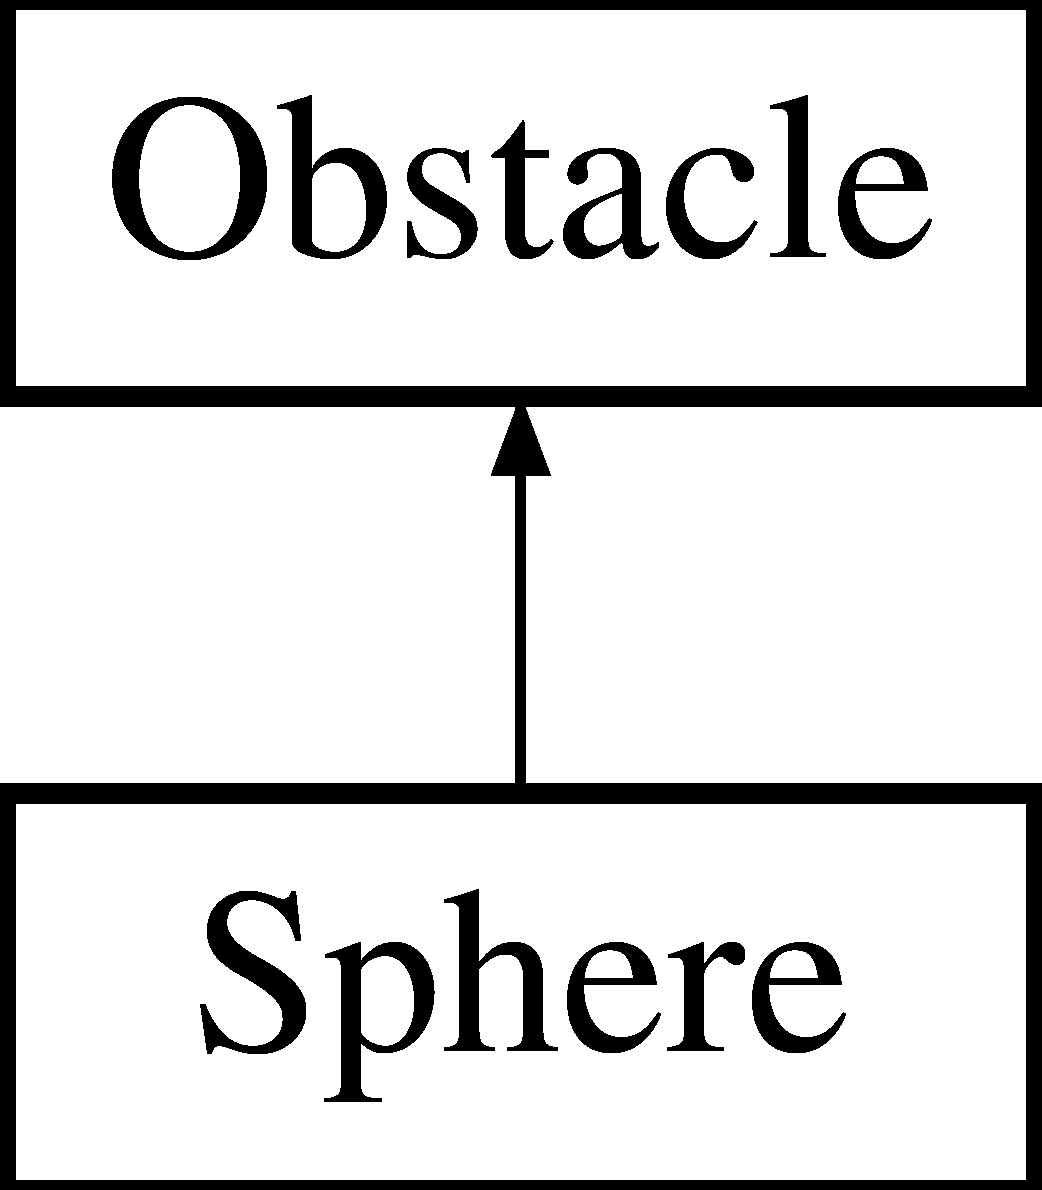
\includegraphics[height=2cm]{classSphere}
\end{center}
\end{figure}
\subsection*{Public Member Functions}
\begin{DoxyCompactItemize}
\item 
\hyperlink{classSphere_a6452552678bc35d4621e3ec9272d34a0}{Sphere} (const ngl::Vec3 \&\_\-pos, const ngl::Colour \&\_\-colour, const ngl::Vec3 \&\_\-size, const std::string \&\_\-shaderName, const struct \hyperlink{structSimulationParams}{SimulationParams} \&\_\-params, \hyperlink{classFluidSystem}{FluidSystem} $\ast$\_\-parent)
\begin{DoxyCompactList}\small\item\em constructor \item\end{DoxyCompactList}\item 
virtual \hyperlink{classSphere_a569c071e50a3e11f678630ee1a17737e}{$\sim$Sphere} ()
\begin{DoxyCompactList}\small\item\em destructor \item\end{DoxyCompactList}\item 
virtual void \hyperlink{classSphere_a75a92a2b70974147560dd8c0514b2652}{draw} () const 
\begin{DoxyCompactList}\small\item\em draw the sphere \item\end{DoxyCompactList}\item 
virtual void \hyperlink{classSphere_a0a18ee7f656154b8c1f60d99bb418c98}{checkCollision} (\hyperlink{classParticle}{Particle} \&\_\-particle)
\begin{DoxyCompactList}\small\item\em collide with a particle \item\end{DoxyCompactList}\end{DoxyCompactItemize}


\subsection{Constructor \& Destructor Documentation}
\hypertarget{classSphere_a6452552678bc35d4621e3ec9272d34a0}{
\index{Sphere@{Sphere}!Sphere@{Sphere}}
\index{Sphere@{Sphere}!Sphere@{Sphere}}
\subsubsection[{Sphere}]{\setlength{\rightskip}{0pt plus 5cm}Sphere::Sphere (const ngl::Vec3 \& {\em \_\-pos}, \/  const ngl::Colour \& {\em \_\-colour}, \/  const ngl::Vec3 \& {\em \_\-size}, \/  const std::string \& {\em \_\-shaderName}, \/  const struct {\bf SimulationParams} \& {\em \_\-params}, \/  {\bf FluidSystem} $\ast$ {\em \_\-parent})}}
\label{classSphere_a6452552678bc35d4621e3ec9272d34a0}


constructor 
\begin{DoxyParams}{Parameters}
\item[\mbox{$\leftarrow$} {\em \_\-pos}]center position of the sphere in world coordinates \item[\mbox{$\leftarrow$} {\em \_\-colour}]color of the sphere \item[\mbox{$\leftarrow$} {\em \_\-size}]dimension fo the sphere \item[\mbox{$\leftarrow$} {\em \_\-shaderName}]shader to use \item[\mbox{$\leftarrow$} {\em \_\-params}]simulation parameters \item[\mbox{$\leftarrow$} {\em \_\-parent}]fluid system to which this obstacle belongs \end{DoxyParams}
\hypertarget{classSphere_a569c071e50a3e11f678630ee1a17737e}{
\index{Sphere@{Sphere}!$\sim$Sphere@{$\sim$Sphere}}
\index{$\sim$Sphere@{$\sim$Sphere}!Sphere@{Sphere}}
\subsubsection[{$\sim$Sphere}]{\setlength{\rightskip}{0pt plus 5cm}Sphere::$\sim$Sphere ()\hspace{0.3cm}{\ttfamily  \mbox{[}virtual\mbox{]}}}}
\label{classSphere_a569c071e50a3e11f678630ee1a17737e}


destructor 

\subsection{Member Function Documentation}
\hypertarget{classSphere_a0a18ee7f656154b8c1f60d99bb418c98}{
\index{Sphere@{Sphere}!checkCollision@{checkCollision}}
\index{checkCollision@{checkCollision}!Sphere@{Sphere}}
\subsubsection[{checkCollision}]{\setlength{\rightskip}{0pt plus 5cm}void Sphere::checkCollision ({\bf Particle} \& {\em \_\-particle})\hspace{0.3cm}{\ttfamily  \mbox{[}virtual\mbox{]}}}}
\label{classSphere_a0a18ee7f656154b8c1f60d99bb418c98}


collide with a particle 
\begin{DoxyParams}{Parameters}
\item[\mbox{$\leftarrow$} {\em \_\-particle}]particle to collide with \end{DoxyParams}


Implements \hyperlink{classObstacle_ae35a1937df593d5caf25c5545acbaffd}{Obstacle}.\hypertarget{classSphere_a75a92a2b70974147560dd8c0514b2652}{
\index{Sphere@{Sphere}!draw@{draw}}
\index{draw@{draw}!Sphere@{Sphere}}
\subsubsection[{draw}]{\setlength{\rightskip}{0pt plus 5cm}void Sphere::draw () const\hspace{0.3cm}{\ttfamily  \mbox{[}virtual\mbox{]}}}}
\label{classSphere_a75a92a2b70974147560dd8c0514b2652}


draw the sphere 

Implements \hyperlink{classObstacle_a7476b22bcd25e3731a0ef2aa5324afa0}{Obstacle}.

The documentation for this class was generated from the following files:\begin{DoxyCompactItemize}
\item 
include/\hyperlink{Sphere_8h}{Sphere.h}\item 
src/\hyperlink{Sphere_8cpp}{Sphere.cpp}\end{DoxyCompactItemize}

\hypertarget{classUi__MainWindow}{
\section{Ui\_\-MainWindow Class Reference}
\label{classUi__MainWindow}\index{Ui\_\-MainWindow@{Ui\_\-MainWindow}}
}


{\ttfamily \#include $<$ui\_\-MainWindow.h$>$}Inheritance diagram for Ui\_\-MainWindow::\begin{figure}[H]
\begin{center}
\leavevmode
\includegraphics[height=2cm]{classUi__MainWindow}
\end{center}
\end{figure}
\subsection*{Public Member Functions}
\begin{DoxyCompactItemize}
\item 
void \hyperlink{classUi__MainWindow_acf4a0872c4c77d8f43a2ec66ed849b58}{setupUi} (QMainWindow $\ast$\hyperlink{classMainWindow}{MainWindow})
\item 
void \hyperlink{classUi__MainWindow_a097dd160c3534a204904cb374412c618}{retranslateUi} (QMainWindow $\ast$\hyperlink{classMainWindow}{MainWindow})
\end{DoxyCompactItemize}
\subsection*{Public Attributes}
\begin{DoxyCompactItemize}
\item 
QWidget $\ast$ \hyperlink{classUi__MainWindow_a356f1cf3ebda15f1fac59467ee081b74}{centralwidget}
\item 
QGridLayout $\ast$ \hyperlink{classUi__MainWindow_ae7902f78acf2ddd14bbda720ac54c450}{s\_\-mainWindowGridLayout}
\item 
QSpacerItem $\ast$ \hyperlink{classUi__MainWindow_a7871ea8c4b6c595d7ccd53960b344719}{horizontalSpacer}
\item 
QGroupBox $\ast$ \hyperlink{classUi__MainWindow_aad6df58cb61e92bd39ce02dcc8a4bd89}{s\_\-paramGB}
\item 
QGridLayout $\ast$ \hyperlink{classUi__MainWindow_a525ed3c5fe0784ac502ee222fba4e205}{gridLayout}
\item 
QLabel $\ast$ \hyperlink{classUi__MainWindow_ad9c89133780f28e6efa2ec17ceb9cff5}{label}
\item 
QDoubleSpinBox $\ast$ \hyperlink{classUi__MainWindow_ad1e34c68f361631331d52954f0da3347}{m\_\-containerSizeZBox}
\item 
QDoubleSpinBox $\ast$ \hyperlink{classUi__MainWindow_a27bcf5d57831be2acc8043f2d6b91916}{m\_\-containerSizeYBox}
\item 
QLabel $\ast$ \hyperlink{classUi__MainWindow_a2e2516d755e4dd53fc905dabddf2738a}{label\_\-2}
\item 
QDoubleSpinBox $\ast$ \hyperlink{classUi__MainWindow_a38f97cea09f884843bb90a7c71093d78}{m\_\-containerSizeXBox}
\item 
QLabel $\ast$ \hyperlink{classUi__MainWindow_a0e90c7e9ad77386881e0b264ddb9dd22}{label\_\-9}
\item 
QDoubleSpinBox $\ast$ \hyperlink{classUi__MainWindow_a4f9f72f5874dab4be00f166117b0adc3}{m\_\-gasKBox}
\item 
QLabel $\ast$ \hyperlink{classUi__MainWindow_a78c7e10730b43c6700cd7216911ed76a}{label\_\-4}
\item 
QDoubleSpinBox $\ast$ \hyperlink{classUi__MainWindow_a8941af0576a2bbc18b2eb4812a0cb957}{m\_\-smoothRadiusBox}
\item 
QLabel $\ast$ \hyperlink{classUi__MainWindow_ad6bab8fb8903b8f41afea1218ee52695}{label\_\-5}
\item 
QDoubleSpinBox $\ast$ \hyperlink{classUi__MainWindow_a223abe14980fe1049e3bbdf0ed376a0a}{m\_\-simulationScaleBox}
\item 
QLabel $\ast$ \hyperlink{classUi__MainWindow_a0376fd90247280e7c7957cc70628708c}{label\_\-3}
\item 
QDoubleSpinBox $\ast$ \hyperlink{classUi__MainWindow_abc208bcf25fb6e90d8952694211f109a}{m\_\-timeStepBox}
\item 
QLabel $\ast$ \hyperlink{classUi__MainWindow_a9dc4dba26b83e0c94aa566e1c564420b}{label\_\-10}
\item 
QDoubleSpinBox $\ast$ \hyperlink{classUi__MainWindow_aed189246fd8fbb26a2ece932b8c03615}{m\_\-tensionBox}
\item 
QLabel $\ast$ \hyperlink{classUi__MainWindow_aa2621565827195e88436fb54220bb48d}{label\_\-12}
\item 
QDoubleSpinBox $\ast$ \hyperlink{classUi__MainWindow_adc503564af3df70c4a6cde0c93a079c2}{m\_\-gravityXBox}
\item 
QDoubleSpinBox $\ast$ \hyperlink{classUi__MainWindow_adddb9f038cf6f566a7cf0ba0802afaf8}{m\_\-gravityYBox}
\item 
QDoubleSpinBox $\ast$ \hyperlink{classUi__MainWindow_aec3524ddb9738f81ad14b0409c23a98c}{m\_\-gravityZBox}
\item 
QLabel $\ast$ \hyperlink{classUi__MainWindow_a663f728e6244926a795c6e6892673b1d}{label\_\-6}
\item 
QDoubleSpinBox $\ast$ \hyperlink{classUi__MainWindow_a7ff20accfdc12db98eeeceaf1bd145b4}{m\_\-restDensityBox}
\item 
QLabel $\ast$ \hyperlink{classUi__MainWindow_af183bfbfb9f38bbdd60caf92b15e23dc}{label\_\-8}
\item 
QDoubleSpinBox $\ast$ \hyperlink{classUi__MainWindow_aed67342868bc3330ef288206a46c2e9f}{m\_\-viscosityBox}
\item 
QPushButton $\ast$ \hyperlink{classUi__MainWindow_a4c6abf58735917e5f2a72face76cbc41}{m\_\-runButton}
\item 
QPushButton $\ast$ \hyperlink{classUi__MainWindow_af0a56879050b5b59965ddb9cc20ad9cc}{m\_\-stopButton}
\item 
QPushButton $\ast$ \hyperlink{classUi__MainWindow_a5caf92edd8ee08153a3d67dd2718429e}{m\_\-resetButton}
\item 
QSpacerItem $\ast$ \hyperlink{classUi__MainWindow_a8384329c3663ff274e926a12024aab52}{verticalSpacer}
\item 
QSpinBox $\ast$ \hyperlink{classUi__MainWindow_a0cedebd0130144b48a6dc129fedd5030}{m\_\-numParticlesBox}
\item 
QLabel $\ast$ \hyperlink{classUi__MainWindow_a882200d8ae16962f5dd3b749ebacbf7e}{label\_\-15}
\item 
QDoubleSpinBox $\ast$ \hyperlink{classUi__MainWindow_adeba4ba7f56681d9962322bb7c8e33f5}{m\_\-elasticityBox}
\item 
QSpacerItem $\ast$ \hyperlink{classUi__MainWindow_ac845bdf6b5b5237378a7b067808b7a31}{verticalSpacer\_\-3}
\item 
QComboBox $\ast$ \hyperlink{classUi__MainWindow_aed4f32d456ab04871cd8d062baec1480}{m\_\-drawBox}
\item 
QLabel $\ast$ \hyperlink{classUi__MainWindow_ab6ac4329a89041f557332f6569d94493}{label\_\-16}
\item 
QLabel $\ast$ \hyperlink{classUi__MainWindow_a1c16c0a684617927472e534822a63c7d}{label\_\-14}
\item 
QSpacerItem $\ast$ \hyperlink{classUi__MainWindow_adc1f5fdd97fb3729999c56902d0fa591}{verticalSpacer\_\-2}
\item 
QSpacerItem $\ast$ \hyperlink{classUi__MainWindow_a298e82ba0cc2500cd61f393f493e4529}{verticalSpacer\_\-4}
\item 
QDoubleSpinBox $\ast$ \hyperlink{classUi__MainWindow_af5fb606a15c63b78d99ef08ffef44bb2}{m\_\-obstacleXBox}
\item 
QDoubleSpinBox $\ast$ \hyperlink{classUi__MainWindow_a91bc8c3fc0d20b7c8bafd4e305d3dbc1}{m\_\-obstacleYBox}
\item 
QDoubleSpinBox $\ast$ \hyperlink{classUi__MainWindow_a63b4ccd5fefd7242fde139d0ced35e24}{m\_\-obstacleZBox}
\item 
QLabel $\ast$ \hyperlink{classUi__MainWindow_a1f4ff90c122fededcc08604401442034}{label\_\-17}
\item 
QDoubleSpinBox $\ast$ \hyperlink{classUi__MainWindow_a683f5df015306268c5135243a234a0ca}{m\_\-obstacleRadiusBox}
\item 
QLabel $\ast$ \hyperlink{classUi__MainWindow_a55100f53189f25cf8a1ee0beb29be642}{label\_\-18}
\item 
QPushButton $\ast$ \hyperlink{classUi__MainWindow_acec2335350b2a00960d8f6dc7a59a2a4}{m\_\-addObstacleButton}
\item 
QPushButton $\ast$ \hyperlink{classUi__MainWindow_ad1aa984f30af3df4d2727e31f38648fa}{m\_\-deleteObstaclesButton}
\item 
QLabel $\ast$ \hyperlink{classUi__MainWindow_a13936e6f18b1c90402b3c7a3c92b6cdb}{label\_\-7}
\item 
QDoubleSpinBox $\ast$ \hyperlink{classUi__MainWindow_a7e35e693ba29d63bbcd1d01556282798}{m\_\-particleMassBox}
\item 
QMenuBar $\ast$ \hyperlink{classUi__MainWindow_adf43d9a67adaec750aaa956b5e082f09}{menubar}
\item 
QStatusBar $\ast$ \hyperlink{classUi__MainWindow_a1687cceb1e2787aa1f83e50433943a91}{statusbar}
\end{DoxyCompactItemize}


\subsection{Member Function Documentation}
\hypertarget{classUi__MainWindow_a097dd160c3534a204904cb374412c618}{
\index{Ui\_\-MainWindow@{Ui\_\-MainWindow}!retranslateUi@{retranslateUi}}
\index{retranslateUi@{retranslateUi}!Ui_MainWindow@{Ui\_\-MainWindow}}
\subsubsection[{retranslateUi}]{\setlength{\rightskip}{0pt plus 5cm}void Ui\_\-MainWindow::retranslateUi (QMainWindow $\ast$ {\em MainWindow})\hspace{0.3cm}{\ttfamily  \mbox{[}inline\mbox{]}}}}
\label{classUi__MainWindow_a097dd160c3534a204904cb374412c618}
\hypertarget{classUi__MainWindow_acf4a0872c4c77d8f43a2ec66ed849b58}{
\index{Ui\_\-MainWindow@{Ui\_\-MainWindow}!setupUi@{setupUi}}
\index{setupUi@{setupUi}!Ui_MainWindow@{Ui\_\-MainWindow}}
\subsubsection[{setupUi}]{\setlength{\rightskip}{0pt plus 5cm}void Ui\_\-MainWindow::setupUi (QMainWindow $\ast$ {\em MainWindow})\hspace{0.3cm}{\ttfamily  \mbox{[}inline\mbox{]}}}}
\label{classUi__MainWindow_acf4a0872c4c77d8f43a2ec66ed849b58}


\subsection{Member Data Documentation}
\hypertarget{classUi__MainWindow_a356f1cf3ebda15f1fac59467ee081b74}{
\index{Ui\_\-MainWindow@{Ui\_\-MainWindow}!centralwidget@{centralwidget}}
\index{centralwidget@{centralwidget}!Ui_MainWindow@{Ui\_\-MainWindow}}
\subsubsection[{centralwidget}]{\setlength{\rightskip}{0pt plus 5cm}QWidget$\ast$ {\bf Ui\_\-MainWindow::centralwidget}}}
\label{classUi__MainWindow_a356f1cf3ebda15f1fac59467ee081b74}
\hypertarget{classUi__MainWindow_a525ed3c5fe0784ac502ee222fba4e205}{
\index{Ui\_\-MainWindow@{Ui\_\-MainWindow}!gridLayout@{gridLayout}}
\index{gridLayout@{gridLayout}!Ui_MainWindow@{Ui\_\-MainWindow}}
\subsubsection[{gridLayout}]{\setlength{\rightskip}{0pt plus 5cm}QGridLayout$\ast$ {\bf Ui\_\-MainWindow::gridLayout}}}
\label{classUi__MainWindow_a525ed3c5fe0784ac502ee222fba4e205}
\hypertarget{classUi__MainWindow_a7871ea8c4b6c595d7ccd53960b344719}{
\index{Ui\_\-MainWindow@{Ui\_\-MainWindow}!horizontalSpacer@{horizontalSpacer}}
\index{horizontalSpacer@{horizontalSpacer}!Ui_MainWindow@{Ui\_\-MainWindow}}
\subsubsection[{horizontalSpacer}]{\setlength{\rightskip}{0pt plus 5cm}QSpacerItem$\ast$ {\bf Ui\_\-MainWindow::horizontalSpacer}}}
\label{classUi__MainWindow_a7871ea8c4b6c595d7ccd53960b344719}
\hypertarget{classUi__MainWindow_ad9c89133780f28e6efa2ec17ceb9cff5}{
\index{Ui\_\-MainWindow@{Ui\_\-MainWindow}!label@{label}}
\index{label@{label}!Ui_MainWindow@{Ui\_\-MainWindow}}
\subsubsection[{label}]{\setlength{\rightskip}{0pt plus 5cm}QLabel$\ast$ {\bf Ui\_\-MainWindow::label}}}
\label{classUi__MainWindow_ad9c89133780f28e6efa2ec17ceb9cff5}
\hypertarget{classUi__MainWindow_a9dc4dba26b83e0c94aa566e1c564420b}{
\index{Ui\_\-MainWindow@{Ui\_\-MainWindow}!label\_\-10@{label\_\-10}}
\index{label\_\-10@{label\_\-10}!Ui_MainWindow@{Ui\_\-MainWindow}}
\subsubsection[{label\_\-10}]{\setlength{\rightskip}{0pt plus 5cm}QLabel$\ast$ {\bf Ui\_\-MainWindow::label\_\-10}}}
\label{classUi__MainWindow_a9dc4dba26b83e0c94aa566e1c564420b}
\hypertarget{classUi__MainWindow_aa2621565827195e88436fb54220bb48d}{
\index{Ui\_\-MainWindow@{Ui\_\-MainWindow}!label\_\-12@{label\_\-12}}
\index{label\_\-12@{label\_\-12}!Ui_MainWindow@{Ui\_\-MainWindow}}
\subsubsection[{label\_\-12}]{\setlength{\rightskip}{0pt plus 5cm}QLabel$\ast$ {\bf Ui\_\-MainWindow::label\_\-12}}}
\label{classUi__MainWindow_aa2621565827195e88436fb54220bb48d}
\hypertarget{classUi__MainWindow_a1c16c0a684617927472e534822a63c7d}{
\index{Ui\_\-MainWindow@{Ui\_\-MainWindow}!label\_\-14@{label\_\-14}}
\index{label\_\-14@{label\_\-14}!Ui_MainWindow@{Ui\_\-MainWindow}}
\subsubsection[{label\_\-14}]{\setlength{\rightskip}{0pt plus 5cm}QLabel$\ast$ {\bf Ui\_\-MainWindow::label\_\-14}}}
\label{classUi__MainWindow_a1c16c0a684617927472e534822a63c7d}
\hypertarget{classUi__MainWindow_a882200d8ae16962f5dd3b749ebacbf7e}{
\index{Ui\_\-MainWindow@{Ui\_\-MainWindow}!label\_\-15@{label\_\-15}}
\index{label\_\-15@{label\_\-15}!Ui_MainWindow@{Ui\_\-MainWindow}}
\subsubsection[{label\_\-15}]{\setlength{\rightskip}{0pt plus 5cm}QLabel$\ast$ {\bf Ui\_\-MainWindow::label\_\-15}}}
\label{classUi__MainWindow_a882200d8ae16962f5dd3b749ebacbf7e}
\hypertarget{classUi__MainWindow_ab6ac4329a89041f557332f6569d94493}{
\index{Ui\_\-MainWindow@{Ui\_\-MainWindow}!label\_\-16@{label\_\-16}}
\index{label\_\-16@{label\_\-16}!Ui_MainWindow@{Ui\_\-MainWindow}}
\subsubsection[{label\_\-16}]{\setlength{\rightskip}{0pt plus 5cm}QLabel$\ast$ {\bf Ui\_\-MainWindow::label\_\-16}}}
\label{classUi__MainWindow_ab6ac4329a89041f557332f6569d94493}
\hypertarget{classUi__MainWindow_a1f4ff90c122fededcc08604401442034}{
\index{Ui\_\-MainWindow@{Ui\_\-MainWindow}!label\_\-17@{label\_\-17}}
\index{label\_\-17@{label\_\-17}!Ui_MainWindow@{Ui\_\-MainWindow}}
\subsubsection[{label\_\-17}]{\setlength{\rightskip}{0pt plus 5cm}QLabel$\ast$ {\bf Ui\_\-MainWindow::label\_\-17}}}
\label{classUi__MainWindow_a1f4ff90c122fededcc08604401442034}
\hypertarget{classUi__MainWindow_a55100f53189f25cf8a1ee0beb29be642}{
\index{Ui\_\-MainWindow@{Ui\_\-MainWindow}!label\_\-18@{label\_\-18}}
\index{label\_\-18@{label\_\-18}!Ui_MainWindow@{Ui\_\-MainWindow}}
\subsubsection[{label\_\-18}]{\setlength{\rightskip}{0pt plus 5cm}QLabel$\ast$ {\bf Ui\_\-MainWindow::label\_\-18}}}
\label{classUi__MainWindow_a55100f53189f25cf8a1ee0beb29be642}
\hypertarget{classUi__MainWindow_a2e2516d755e4dd53fc905dabddf2738a}{
\index{Ui\_\-MainWindow@{Ui\_\-MainWindow}!label\_\-2@{label\_\-2}}
\index{label\_\-2@{label\_\-2}!Ui_MainWindow@{Ui\_\-MainWindow}}
\subsubsection[{label\_\-2}]{\setlength{\rightskip}{0pt plus 5cm}QLabel$\ast$ {\bf Ui\_\-MainWindow::label\_\-2}}}
\label{classUi__MainWindow_a2e2516d755e4dd53fc905dabddf2738a}
\hypertarget{classUi__MainWindow_a0376fd90247280e7c7957cc70628708c}{
\index{Ui\_\-MainWindow@{Ui\_\-MainWindow}!label\_\-3@{label\_\-3}}
\index{label\_\-3@{label\_\-3}!Ui_MainWindow@{Ui\_\-MainWindow}}
\subsubsection[{label\_\-3}]{\setlength{\rightskip}{0pt plus 5cm}QLabel$\ast$ {\bf Ui\_\-MainWindow::label\_\-3}}}
\label{classUi__MainWindow_a0376fd90247280e7c7957cc70628708c}
\hypertarget{classUi__MainWindow_a78c7e10730b43c6700cd7216911ed76a}{
\index{Ui\_\-MainWindow@{Ui\_\-MainWindow}!label\_\-4@{label\_\-4}}
\index{label\_\-4@{label\_\-4}!Ui_MainWindow@{Ui\_\-MainWindow}}
\subsubsection[{label\_\-4}]{\setlength{\rightskip}{0pt plus 5cm}QLabel$\ast$ {\bf Ui\_\-MainWindow::label\_\-4}}}
\label{classUi__MainWindow_a78c7e10730b43c6700cd7216911ed76a}
\hypertarget{classUi__MainWindow_ad6bab8fb8903b8f41afea1218ee52695}{
\index{Ui\_\-MainWindow@{Ui\_\-MainWindow}!label\_\-5@{label\_\-5}}
\index{label\_\-5@{label\_\-5}!Ui_MainWindow@{Ui\_\-MainWindow}}
\subsubsection[{label\_\-5}]{\setlength{\rightskip}{0pt plus 5cm}QLabel$\ast$ {\bf Ui\_\-MainWindow::label\_\-5}}}
\label{classUi__MainWindow_ad6bab8fb8903b8f41afea1218ee52695}
\hypertarget{classUi__MainWindow_a663f728e6244926a795c6e6892673b1d}{
\index{Ui\_\-MainWindow@{Ui\_\-MainWindow}!label\_\-6@{label\_\-6}}
\index{label\_\-6@{label\_\-6}!Ui_MainWindow@{Ui\_\-MainWindow}}
\subsubsection[{label\_\-6}]{\setlength{\rightskip}{0pt plus 5cm}QLabel$\ast$ {\bf Ui\_\-MainWindow::label\_\-6}}}
\label{classUi__MainWindow_a663f728e6244926a795c6e6892673b1d}
\hypertarget{classUi__MainWindow_a13936e6f18b1c90402b3c7a3c92b6cdb}{
\index{Ui\_\-MainWindow@{Ui\_\-MainWindow}!label\_\-7@{label\_\-7}}
\index{label\_\-7@{label\_\-7}!Ui_MainWindow@{Ui\_\-MainWindow}}
\subsubsection[{label\_\-7}]{\setlength{\rightskip}{0pt plus 5cm}QLabel$\ast$ {\bf Ui\_\-MainWindow::label\_\-7}}}
\label{classUi__MainWindow_a13936e6f18b1c90402b3c7a3c92b6cdb}
\hypertarget{classUi__MainWindow_af183bfbfb9f38bbdd60caf92b15e23dc}{
\index{Ui\_\-MainWindow@{Ui\_\-MainWindow}!label\_\-8@{label\_\-8}}
\index{label\_\-8@{label\_\-8}!Ui_MainWindow@{Ui\_\-MainWindow}}
\subsubsection[{label\_\-8}]{\setlength{\rightskip}{0pt plus 5cm}QLabel$\ast$ {\bf Ui\_\-MainWindow::label\_\-8}}}
\label{classUi__MainWindow_af183bfbfb9f38bbdd60caf92b15e23dc}
\hypertarget{classUi__MainWindow_a0e90c7e9ad77386881e0b264ddb9dd22}{
\index{Ui\_\-MainWindow@{Ui\_\-MainWindow}!label\_\-9@{label\_\-9}}
\index{label\_\-9@{label\_\-9}!Ui_MainWindow@{Ui\_\-MainWindow}}
\subsubsection[{label\_\-9}]{\setlength{\rightskip}{0pt plus 5cm}QLabel$\ast$ {\bf Ui\_\-MainWindow::label\_\-9}}}
\label{classUi__MainWindow_a0e90c7e9ad77386881e0b264ddb9dd22}
\hypertarget{classUi__MainWindow_acec2335350b2a00960d8f6dc7a59a2a4}{
\index{Ui\_\-MainWindow@{Ui\_\-MainWindow}!m\_\-addObstacleButton@{m\_\-addObstacleButton}}
\index{m\_\-addObstacleButton@{m\_\-addObstacleButton}!Ui_MainWindow@{Ui\_\-MainWindow}}
\subsubsection[{m\_\-addObstacleButton}]{\setlength{\rightskip}{0pt plus 5cm}QPushButton$\ast$ {\bf Ui\_\-MainWindow::m\_\-addObstacleButton}}}
\label{classUi__MainWindow_acec2335350b2a00960d8f6dc7a59a2a4}
\hypertarget{classUi__MainWindow_a38f97cea09f884843bb90a7c71093d78}{
\index{Ui\_\-MainWindow@{Ui\_\-MainWindow}!m\_\-containerSizeXBox@{m\_\-containerSizeXBox}}
\index{m\_\-containerSizeXBox@{m\_\-containerSizeXBox}!Ui_MainWindow@{Ui\_\-MainWindow}}
\subsubsection[{m\_\-containerSizeXBox}]{\setlength{\rightskip}{0pt plus 5cm}QDoubleSpinBox$\ast$ {\bf Ui\_\-MainWindow::m\_\-containerSizeXBox}}}
\label{classUi__MainWindow_a38f97cea09f884843bb90a7c71093d78}
\hypertarget{classUi__MainWindow_a27bcf5d57831be2acc8043f2d6b91916}{
\index{Ui\_\-MainWindow@{Ui\_\-MainWindow}!m\_\-containerSizeYBox@{m\_\-containerSizeYBox}}
\index{m\_\-containerSizeYBox@{m\_\-containerSizeYBox}!Ui_MainWindow@{Ui\_\-MainWindow}}
\subsubsection[{m\_\-containerSizeYBox}]{\setlength{\rightskip}{0pt plus 5cm}QDoubleSpinBox$\ast$ {\bf Ui\_\-MainWindow::m\_\-containerSizeYBox}}}
\label{classUi__MainWindow_a27bcf5d57831be2acc8043f2d6b91916}
\hypertarget{classUi__MainWindow_ad1e34c68f361631331d52954f0da3347}{
\index{Ui\_\-MainWindow@{Ui\_\-MainWindow}!m\_\-containerSizeZBox@{m\_\-containerSizeZBox}}
\index{m\_\-containerSizeZBox@{m\_\-containerSizeZBox}!Ui_MainWindow@{Ui\_\-MainWindow}}
\subsubsection[{m\_\-containerSizeZBox}]{\setlength{\rightskip}{0pt plus 5cm}QDoubleSpinBox$\ast$ {\bf Ui\_\-MainWindow::m\_\-containerSizeZBox}}}
\label{classUi__MainWindow_ad1e34c68f361631331d52954f0da3347}
\hypertarget{classUi__MainWindow_ad1aa984f30af3df4d2727e31f38648fa}{
\index{Ui\_\-MainWindow@{Ui\_\-MainWindow}!m\_\-deleteObstaclesButton@{m\_\-deleteObstaclesButton}}
\index{m\_\-deleteObstaclesButton@{m\_\-deleteObstaclesButton}!Ui_MainWindow@{Ui\_\-MainWindow}}
\subsubsection[{m\_\-deleteObstaclesButton}]{\setlength{\rightskip}{0pt plus 5cm}QPushButton$\ast$ {\bf Ui\_\-MainWindow::m\_\-deleteObstaclesButton}}}
\label{classUi__MainWindow_ad1aa984f30af3df4d2727e31f38648fa}
\hypertarget{classUi__MainWindow_aed4f32d456ab04871cd8d062baec1480}{
\index{Ui\_\-MainWindow@{Ui\_\-MainWindow}!m\_\-drawBox@{m\_\-drawBox}}
\index{m\_\-drawBox@{m\_\-drawBox}!Ui_MainWindow@{Ui\_\-MainWindow}}
\subsubsection[{m\_\-drawBox}]{\setlength{\rightskip}{0pt plus 5cm}QComboBox$\ast$ {\bf Ui\_\-MainWindow::m\_\-drawBox}}}
\label{classUi__MainWindow_aed4f32d456ab04871cd8d062baec1480}
\hypertarget{classUi__MainWindow_adeba4ba7f56681d9962322bb7c8e33f5}{
\index{Ui\_\-MainWindow@{Ui\_\-MainWindow}!m\_\-elasticityBox@{m\_\-elasticityBox}}
\index{m\_\-elasticityBox@{m\_\-elasticityBox}!Ui_MainWindow@{Ui\_\-MainWindow}}
\subsubsection[{m\_\-elasticityBox}]{\setlength{\rightskip}{0pt plus 5cm}QDoubleSpinBox$\ast$ {\bf Ui\_\-MainWindow::m\_\-elasticityBox}}}
\label{classUi__MainWindow_adeba4ba7f56681d9962322bb7c8e33f5}
\hypertarget{classUi__MainWindow_a4f9f72f5874dab4be00f166117b0adc3}{
\index{Ui\_\-MainWindow@{Ui\_\-MainWindow}!m\_\-gasKBox@{m\_\-gasKBox}}
\index{m\_\-gasKBox@{m\_\-gasKBox}!Ui_MainWindow@{Ui\_\-MainWindow}}
\subsubsection[{m\_\-gasKBox}]{\setlength{\rightskip}{0pt plus 5cm}QDoubleSpinBox$\ast$ {\bf Ui\_\-MainWindow::m\_\-gasKBox}}}
\label{classUi__MainWindow_a4f9f72f5874dab4be00f166117b0adc3}
\hypertarget{classUi__MainWindow_adc503564af3df70c4a6cde0c93a079c2}{
\index{Ui\_\-MainWindow@{Ui\_\-MainWindow}!m\_\-gravityXBox@{m\_\-gravityXBox}}
\index{m\_\-gravityXBox@{m\_\-gravityXBox}!Ui_MainWindow@{Ui\_\-MainWindow}}
\subsubsection[{m\_\-gravityXBox}]{\setlength{\rightskip}{0pt plus 5cm}QDoubleSpinBox$\ast$ {\bf Ui\_\-MainWindow::m\_\-gravityXBox}}}
\label{classUi__MainWindow_adc503564af3df70c4a6cde0c93a079c2}
\hypertarget{classUi__MainWindow_adddb9f038cf6f566a7cf0ba0802afaf8}{
\index{Ui\_\-MainWindow@{Ui\_\-MainWindow}!m\_\-gravityYBox@{m\_\-gravityYBox}}
\index{m\_\-gravityYBox@{m\_\-gravityYBox}!Ui_MainWindow@{Ui\_\-MainWindow}}
\subsubsection[{m\_\-gravityYBox}]{\setlength{\rightskip}{0pt plus 5cm}QDoubleSpinBox$\ast$ {\bf Ui\_\-MainWindow::m\_\-gravityYBox}}}
\label{classUi__MainWindow_adddb9f038cf6f566a7cf0ba0802afaf8}
\hypertarget{classUi__MainWindow_aec3524ddb9738f81ad14b0409c23a98c}{
\index{Ui\_\-MainWindow@{Ui\_\-MainWindow}!m\_\-gravityZBox@{m\_\-gravityZBox}}
\index{m\_\-gravityZBox@{m\_\-gravityZBox}!Ui_MainWindow@{Ui\_\-MainWindow}}
\subsubsection[{m\_\-gravityZBox}]{\setlength{\rightskip}{0pt plus 5cm}QDoubleSpinBox$\ast$ {\bf Ui\_\-MainWindow::m\_\-gravityZBox}}}
\label{classUi__MainWindow_aec3524ddb9738f81ad14b0409c23a98c}
\hypertarget{classUi__MainWindow_a0cedebd0130144b48a6dc129fedd5030}{
\index{Ui\_\-MainWindow@{Ui\_\-MainWindow}!m\_\-numParticlesBox@{m\_\-numParticlesBox}}
\index{m\_\-numParticlesBox@{m\_\-numParticlesBox}!Ui_MainWindow@{Ui\_\-MainWindow}}
\subsubsection[{m\_\-numParticlesBox}]{\setlength{\rightskip}{0pt plus 5cm}QSpinBox$\ast$ {\bf Ui\_\-MainWindow::m\_\-numParticlesBox}}}
\label{classUi__MainWindow_a0cedebd0130144b48a6dc129fedd5030}
\hypertarget{classUi__MainWindow_a683f5df015306268c5135243a234a0ca}{
\index{Ui\_\-MainWindow@{Ui\_\-MainWindow}!m\_\-obstacleRadiusBox@{m\_\-obstacleRadiusBox}}
\index{m\_\-obstacleRadiusBox@{m\_\-obstacleRadiusBox}!Ui_MainWindow@{Ui\_\-MainWindow}}
\subsubsection[{m\_\-obstacleRadiusBox}]{\setlength{\rightskip}{0pt plus 5cm}QDoubleSpinBox$\ast$ {\bf Ui\_\-MainWindow::m\_\-obstacleRadiusBox}}}
\label{classUi__MainWindow_a683f5df015306268c5135243a234a0ca}
\hypertarget{classUi__MainWindow_af5fb606a15c63b78d99ef08ffef44bb2}{
\index{Ui\_\-MainWindow@{Ui\_\-MainWindow}!m\_\-obstacleXBox@{m\_\-obstacleXBox}}
\index{m\_\-obstacleXBox@{m\_\-obstacleXBox}!Ui_MainWindow@{Ui\_\-MainWindow}}
\subsubsection[{m\_\-obstacleXBox}]{\setlength{\rightskip}{0pt plus 5cm}QDoubleSpinBox$\ast$ {\bf Ui\_\-MainWindow::m\_\-obstacleXBox}}}
\label{classUi__MainWindow_af5fb606a15c63b78d99ef08ffef44bb2}
\hypertarget{classUi__MainWindow_a91bc8c3fc0d20b7c8bafd4e305d3dbc1}{
\index{Ui\_\-MainWindow@{Ui\_\-MainWindow}!m\_\-obstacleYBox@{m\_\-obstacleYBox}}
\index{m\_\-obstacleYBox@{m\_\-obstacleYBox}!Ui_MainWindow@{Ui\_\-MainWindow}}
\subsubsection[{m\_\-obstacleYBox}]{\setlength{\rightskip}{0pt plus 5cm}QDoubleSpinBox$\ast$ {\bf Ui\_\-MainWindow::m\_\-obstacleYBox}}}
\label{classUi__MainWindow_a91bc8c3fc0d20b7c8bafd4e305d3dbc1}
\hypertarget{classUi__MainWindow_a63b4ccd5fefd7242fde139d0ced35e24}{
\index{Ui\_\-MainWindow@{Ui\_\-MainWindow}!m\_\-obstacleZBox@{m\_\-obstacleZBox}}
\index{m\_\-obstacleZBox@{m\_\-obstacleZBox}!Ui_MainWindow@{Ui\_\-MainWindow}}
\subsubsection[{m\_\-obstacleZBox}]{\setlength{\rightskip}{0pt plus 5cm}QDoubleSpinBox$\ast$ {\bf Ui\_\-MainWindow::m\_\-obstacleZBox}}}
\label{classUi__MainWindow_a63b4ccd5fefd7242fde139d0ced35e24}
\hypertarget{classUi__MainWindow_a7e35e693ba29d63bbcd1d01556282798}{
\index{Ui\_\-MainWindow@{Ui\_\-MainWindow}!m\_\-particleMassBox@{m\_\-particleMassBox}}
\index{m\_\-particleMassBox@{m\_\-particleMassBox}!Ui_MainWindow@{Ui\_\-MainWindow}}
\subsubsection[{m\_\-particleMassBox}]{\setlength{\rightskip}{0pt plus 5cm}QDoubleSpinBox$\ast$ {\bf Ui\_\-MainWindow::m\_\-particleMassBox}}}
\label{classUi__MainWindow_a7e35e693ba29d63bbcd1d01556282798}
\hypertarget{classUi__MainWindow_a5caf92edd8ee08153a3d67dd2718429e}{
\index{Ui\_\-MainWindow@{Ui\_\-MainWindow}!m\_\-resetButton@{m\_\-resetButton}}
\index{m\_\-resetButton@{m\_\-resetButton}!Ui_MainWindow@{Ui\_\-MainWindow}}
\subsubsection[{m\_\-resetButton}]{\setlength{\rightskip}{0pt plus 5cm}QPushButton$\ast$ {\bf Ui\_\-MainWindow::m\_\-resetButton}}}
\label{classUi__MainWindow_a5caf92edd8ee08153a3d67dd2718429e}
\hypertarget{classUi__MainWindow_a7ff20accfdc12db98eeeceaf1bd145b4}{
\index{Ui\_\-MainWindow@{Ui\_\-MainWindow}!m\_\-restDensityBox@{m\_\-restDensityBox}}
\index{m\_\-restDensityBox@{m\_\-restDensityBox}!Ui_MainWindow@{Ui\_\-MainWindow}}
\subsubsection[{m\_\-restDensityBox}]{\setlength{\rightskip}{0pt plus 5cm}QDoubleSpinBox$\ast$ {\bf Ui\_\-MainWindow::m\_\-restDensityBox}}}
\label{classUi__MainWindow_a7ff20accfdc12db98eeeceaf1bd145b4}
\hypertarget{classUi__MainWindow_a4c6abf58735917e5f2a72face76cbc41}{
\index{Ui\_\-MainWindow@{Ui\_\-MainWindow}!m\_\-runButton@{m\_\-runButton}}
\index{m\_\-runButton@{m\_\-runButton}!Ui_MainWindow@{Ui\_\-MainWindow}}
\subsubsection[{m\_\-runButton}]{\setlength{\rightskip}{0pt plus 5cm}QPushButton$\ast$ {\bf Ui\_\-MainWindow::m\_\-runButton}}}
\label{classUi__MainWindow_a4c6abf58735917e5f2a72face76cbc41}
\hypertarget{classUi__MainWindow_a223abe14980fe1049e3bbdf0ed376a0a}{
\index{Ui\_\-MainWindow@{Ui\_\-MainWindow}!m\_\-simulationScaleBox@{m\_\-simulationScaleBox}}
\index{m\_\-simulationScaleBox@{m\_\-simulationScaleBox}!Ui_MainWindow@{Ui\_\-MainWindow}}
\subsubsection[{m\_\-simulationScaleBox}]{\setlength{\rightskip}{0pt plus 5cm}QDoubleSpinBox$\ast$ {\bf Ui\_\-MainWindow::m\_\-simulationScaleBox}}}
\label{classUi__MainWindow_a223abe14980fe1049e3bbdf0ed376a0a}
\hypertarget{classUi__MainWindow_a8941af0576a2bbc18b2eb4812a0cb957}{
\index{Ui\_\-MainWindow@{Ui\_\-MainWindow}!m\_\-smoothRadiusBox@{m\_\-smoothRadiusBox}}
\index{m\_\-smoothRadiusBox@{m\_\-smoothRadiusBox}!Ui_MainWindow@{Ui\_\-MainWindow}}
\subsubsection[{m\_\-smoothRadiusBox}]{\setlength{\rightskip}{0pt plus 5cm}QDoubleSpinBox$\ast$ {\bf Ui\_\-MainWindow::m\_\-smoothRadiusBox}}}
\label{classUi__MainWindow_a8941af0576a2bbc18b2eb4812a0cb957}
\hypertarget{classUi__MainWindow_af0a56879050b5b59965ddb9cc20ad9cc}{
\index{Ui\_\-MainWindow@{Ui\_\-MainWindow}!m\_\-stopButton@{m\_\-stopButton}}
\index{m\_\-stopButton@{m\_\-stopButton}!Ui_MainWindow@{Ui\_\-MainWindow}}
\subsubsection[{m\_\-stopButton}]{\setlength{\rightskip}{0pt plus 5cm}QPushButton$\ast$ {\bf Ui\_\-MainWindow::m\_\-stopButton}}}
\label{classUi__MainWindow_af0a56879050b5b59965ddb9cc20ad9cc}
\hypertarget{classUi__MainWindow_aed189246fd8fbb26a2ece932b8c03615}{
\index{Ui\_\-MainWindow@{Ui\_\-MainWindow}!m\_\-tensionBox@{m\_\-tensionBox}}
\index{m\_\-tensionBox@{m\_\-tensionBox}!Ui_MainWindow@{Ui\_\-MainWindow}}
\subsubsection[{m\_\-tensionBox}]{\setlength{\rightskip}{0pt plus 5cm}QDoubleSpinBox$\ast$ {\bf Ui\_\-MainWindow::m\_\-tensionBox}}}
\label{classUi__MainWindow_aed189246fd8fbb26a2ece932b8c03615}
\hypertarget{classUi__MainWindow_abc208bcf25fb6e90d8952694211f109a}{
\index{Ui\_\-MainWindow@{Ui\_\-MainWindow}!m\_\-timeStepBox@{m\_\-timeStepBox}}
\index{m\_\-timeStepBox@{m\_\-timeStepBox}!Ui_MainWindow@{Ui\_\-MainWindow}}
\subsubsection[{m\_\-timeStepBox}]{\setlength{\rightskip}{0pt plus 5cm}QDoubleSpinBox$\ast$ {\bf Ui\_\-MainWindow::m\_\-timeStepBox}}}
\label{classUi__MainWindow_abc208bcf25fb6e90d8952694211f109a}
\hypertarget{classUi__MainWindow_aed67342868bc3330ef288206a46c2e9f}{
\index{Ui\_\-MainWindow@{Ui\_\-MainWindow}!m\_\-viscosityBox@{m\_\-viscosityBox}}
\index{m\_\-viscosityBox@{m\_\-viscosityBox}!Ui_MainWindow@{Ui\_\-MainWindow}}
\subsubsection[{m\_\-viscosityBox}]{\setlength{\rightskip}{0pt plus 5cm}QDoubleSpinBox$\ast$ {\bf Ui\_\-MainWindow::m\_\-viscosityBox}}}
\label{classUi__MainWindow_aed67342868bc3330ef288206a46c2e9f}
\hypertarget{classUi__MainWindow_adf43d9a67adaec750aaa956b5e082f09}{
\index{Ui\_\-MainWindow@{Ui\_\-MainWindow}!menubar@{menubar}}
\index{menubar@{menubar}!Ui_MainWindow@{Ui\_\-MainWindow}}
\subsubsection[{menubar}]{\setlength{\rightskip}{0pt plus 5cm}QMenuBar$\ast$ {\bf Ui\_\-MainWindow::menubar}}}
\label{classUi__MainWindow_adf43d9a67adaec750aaa956b5e082f09}
\hypertarget{classUi__MainWindow_ae7902f78acf2ddd14bbda720ac54c450}{
\index{Ui\_\-MainWindow@{Ui\_\-MainWindow}!s\_\-mainWindowGridLayout@{s\_\-mainWindowGridLayout}}
\index{s\_\-mainWindowGridLayout@{s\_\-mainWindowGridLayout}!Ui_MainWindow@{Ui\_\-MainWindow}}
\subsubsection[{s\_\-mainWindowGridLayout}]{\setlength{\rightskip}{0pt plus 5cm}QGridLayout$\ast$ {\bf Ui\_\-MainWindow::s\_\-mainWindowGridLayout}}}
\label{classUi__MainWindow_ae7902f78acf2ddd14bbda720ac54c450}
\hypertarget{classUi__MainWindow_aad6df58cb61e92bd39ce02dcc8a4bd89}{
\index{Ui\_\-MainWindow@{Ui\_\-MainWindow}!s\_\-paramGB@{s\_\-paramGB}}
\index{s\_\-paramGB@{s\_\-paramGB}!Ui_MainWindow@{Ui\_\-MainWindow}}
\subsubsection[{s\_\-paramGB}]{\setlength{\rightskip}{0pt plus 5cm}QGroupBox$\ast$ {\bf Ui\_\-MainWindow::s\_\-paramGB}}}
\label{classUi__MainWindow_aad6df58cb61e92bd39ce02dcc8a4bd89}
\hypertarget{classUi__MainWindow_a1687cceb1e2787aa1f83e50433943a91}{
\index{Ui\_\-MainWindow@{Ui\_\-MainWindow}!statusbar@{statusbar}}
\index{statusbar@{statusbar}!Ui_MainWindow@{Ui\_\-MainWindow}}
\subsubsection[{statusbar}]{\setlength{\rightskip}{0pt plus 5cm}QStatusBar$\ast$ {\bf Ui\_\-MainWindow::statusbar}}}
\label{classUi__MainWindow_a1687cceb1e2787aa1f83e50433943a91}
\hypertarget{classUi__MainWindow_a8384329c3663ff274e926a12024aab52}{
\index{Ui\_\-MainWindow@{Ui\_\-MainWindow}!verticalSpacer@{verticalSpacer}}
\index{verticalSpacer@{verticalSpacer}!Ui_MainWindow@{Ui\_\-MainWindow}}
\subsubsection[{verticalSpacer}]{\setlength{\rightskip}{0pt plus 5cm}QSpacerItem$\ast$ {\bf Ui\_\-MainWindow::verticalSpacer}}}
\label{classUi__MainWindow_a8384329c3663ff274e926a12024aab52}
\hypertarget{classUi__MainWindow_adc1f5fdd97fb3729999c56902d0fa591}{
\index{Ui\_\-MainWindow@{Ui\_\-MainWindow}!verticalSpacer\_\-2@{verticalSpacer\_\-2}}
\index{verticalSpacer\_\-2@{verticalSpacer\_\-2}!Ui_MainWindow@{Ui\_\-MainWindow}}
\subsubsection[{verticalSpacer\_\-2}]{\setlength{\rightskip}{0pt plus 5cm}QSpacerItem$\ast$ {\bf Ui\_\-MainWindow::verticalSpacer\_\-2}}}
\label{classUi__MainWindow_adc1f5fdd97fb3729999c56902d0fa591}
\hypertarget{classUi__MainWindow_ac845bdf6b5b5237378a7b067808b7a31}{
\index{Ui\_\-MainWindow@{Ui\_\-MainWindow}!verticalSpacer\_\-3@{verticalSpacer\_\-3}}
\index{verticalSpacer\_\-3@{verticalSpacer\_\-3}!Ui_MainWindow@{Ui\_\-MainWindow}}
\subsubsection[{verticalSpacer\_\-3}]{\setlength{\rightskip}{0pt plus 5cm}QSpacerItem$\ast$ {\bf Ui\_\-MainWindow::verticalSpacer\_\-3}}}
\label{classUi__MainWindow_ac845bdf6b5b5237378a7b067808b7a31}
\hypertarget{classUi__MainWindow_a298e82ba0cc2500cd61f393f493e4529}{
\index{Ui\_\-MainWindow@{Ui\_\-MainWindow}!verticalSpacer\_\-4@{verticalSpacer\_\-4}}
\index{verticalSpacer\_\-4@{verticalSpacer\_\-4}!Ui_MainWindow@{Ui\_\-MainWindow}}
\subsubsection[{verticalSpacer\_\-4}]{\setlength{\rightskip}{0pt plus 5cm}QSpacerItem$\ast$ {\bf Ui\_\-MainWindow::verticalSpacer\_\-4}}}
\label{classUi__MainWindow_a298e82ba0cc2500cd61f393f493e4529}


The documentation for this class was generated from the following file:\begin{DoxyCompactItemize}
\item 
ui/\hyperlink{ui__MainWindow_8h}{ui\_\-MainWindow.h}\end{DoxyCompactItemize}

\chapter{File Documentation}
\hypertarget{Common_8h}{
\section{include/Common.h File Reference}
\label{Common_8h}\index{include/Common.h@{include/Common.h}}
}


Header file for common definitions used throughout the system.  
{\ttfamily \#include $<$cstdlib$>$}\par
{\ttfamily \#include $<$ngl/Vec3.h$>$}\par
\subsection*{Classes}
\begin{DoxyCompactItemize}
\item 
struct \hyperlink{structSimulationParams}{SimulationParams}
\begin{DoxyCompactList}\small\item\em store parsed parameters for the system \item\end{DoxyCompactList}\item 
struct \hyperlink{structFluidParams}{FluidParams}
\begin{DoxyCompactList}\small\item\em store parsed parameters for fluid \item\end{DoxyCompactList}\end{DoxyCompactItemize}
\subsection*{Defines}
\begin{DoxyCompactItemize}
\item 
\#define \hyperlink{Common_8h_ad72dbcf6d0153db1b8d8a58001feed83}{DEBUG}~0
\begin{DoxyCompactList}\small\item\em debug flag definition from Gianni at Stack Overflow \href{http://stackoverflow.com/questions/3371540/c-enable-disable-debug-messages-of-stdcouts-on-the-fly}{\tt http://stackoverflow.com/questions/3371540/c-\/enable-\/disable-\/debug-\/messages-\/of-\/stdcouts-\/on-\/the-\/fly} \item\end{DoxyCompactList}\item 
\#define \hyperlink{Common_8h_af1206b4d3bda8c4c8c9257f369a9e9e1}{DEBUG\_\-MSG}(str)~do \{ \} while ( false )
\item 
\#define \hyperlink{Common_8h_a002b2f4894492820fe708b1b7e7c5e70}{EPSILON}~0.0001
\begin{DoxyCompactList}\small\item\em error margin for collision tests \item\end{DoxyCompactList}\end{DoxyCompactItemize}
\subsection*{Enumerations}
\begin{DoxyCompactItemize}
\item 
enum \hyperlink{Common_8h_a9a325db332d24e6105fe3b48a94604c3}{DrawMode} \{ \hyperlink{Common_8h_a9a325db332d24e6105fe3b48a94604c3adc0f401e772f1affa81071e70631abbf}{POINTS}, 
\hyperlink{Common_8h_a9a325db332d24e6105fe3b48a94604c3a9d2cc316ab2e6e5637281696bebc6ffd}{DENSITY}, 
\hyperlink{Common_8h_a9a325db332d24e6105fe3b48a94604c3aa2b65445a3a16f164c5e811064d75726}{RANDOM}, 
\hyperlink{Common_8h_a9a325db332d24e6105fe3b48a94604c3a06e15744a8bd69fceeeb39ab3614b3f6}{VELOCITY}
 \}
\item 
enum \hyperlink{Common_8h_a9852a22595ceae4debd70f078e037971}{ObstacleType} \{ \hyperlink{Common_8h_a9852a22595ceae4debd70f078e037971aae4f0962d104ea473feec5598689316d}{SPHERE}, 
\hyperlink{Common_8h_a9852a22595ceae4debd70f078e037971ad9ff273a12ff18b3e1b900080aadd1ea}{CUBE}
 \}
\end{DoxyCompactItemize}
\subsection*{Functions}
\begin{DoxyCompactItemize}
\item 
{\footnotesize template$<$class T $>$ }\\T \hyperlink{Common_8h_ae46541f98ab0618cbfe51fb1d01e3774}{Sign} (T \_\-a)
\end{DoxyCompactItemize}


\subsection{Detailed Description}
Header file for common definitions used throughout the system. \begin{DoxyAuthor}{Author}
Julia Lou 
\end{DoxyAuthor}
\begin{DoxyDate}{Date}
26/03/2013 
\end{DoxyDate}


\subsection{Define Documentation}
\hypertarget{Common_8h_ad72dbcf6d0153db1b8d8a58001feed83}{
\index{Common.h@{Common.h}!DEBUG@{DEBUG}}
\index{DEBUG@{DEBUG}!Common.h@{Common.h}}
\subsubsection[{DEBUG}]{\setlength{\rightskip}{0pt plus 5cm}\#define DEBUG~0}}
\label{Common_8h_ad72dbcf6d0153db1b8d8a58001feed83}


debug flag definition from Gianni at Stack Overflow \href{http://stackoverflow.com/questions/3371540/c-enable-disable-debug-messages-of-stdcouts-on-the-fly}{\tt http://stackoverflow.com/questions/3371540/c-\/enable-\/disable-\/debug-\/messages-\/of-\/stdcouts-\/on-\/the-\/fly} \hypertarget{Common_8h_af1206b4d3bda8c4c8c9257f369a9e9e1}{
\index{Common.h@{Common.h}!DEBUG\_\-MSG@{DEBUG\_\-MSG}}
\index{DEBUG\_\-MSG@{DEBUG\_\-MSG}!Common.h@{Common.h}}
\subsubsection[{DEBUG\_\-MSG}]{\setlength{\rightskip}{0pt plus 5cm}\#define DEBUG\_\-MSG(str)~do \{ \} while ( false )}}
\label{Common_8h_af1206b4d3bda8c4c8c9257f369a9e9e1}
\hypertarget{Common_8h_a002b2f4894492820fe708b1b7e7c5e70}{
\index{Common.h@{Common.h}!EPSILON@{EPSILON}}
\index{EPSILON@{EPSILON}!Common.h@{Common.h}}
\subsubsection[{EPSILON}]{\setlength{\rightskip}{0pt plus 5cm}\#define EPSILON~0.0001}}
\label{Common_8h_a002b2f4894492820fe708b1b7e7c5e70}


error margin for collision tests 

\subsection{Enumeration Type Documentation}
\hypertarget{Common_8h_a9a325db332d24e6105fe3b48a94604c3}{
\index{Common.h@{Common.h}!DrawMode@{DrawMode}}
\index{DrawMode@{DrawMode}!Common.h@{Common.h}}
\subsubsection[{DrawMode}]{\setlength{\rightskip}{0pt plus 5cm}enum {\bf DrawMode}}}
\label{Common_8h_a9a325db332d24e6105fe3b48a94604c3}
\begin{Desc}
\item[Enumerator: ]\par
\begin{description}
\index{POINTS@{POINTS}!Common.h@{Common.h}}\index{Common.h@{Common.h}!POINTS@{POINTS}}\item[{\em 
\hypertarget{Common_8h_a9a325db332d24e6105fe3b48a94604c3adc0f401e772f1affa81071e70631abbf}{
POINTS}
\label{Common_8h_a9a325db332d24e6105fe3b48a94604c3adc0f401e772f1affa81071e70631abbf}
}]\index{DENSITY@{DENSITY}!Common.h@{Common.h}}\index{Common.h@{Common.h}!DENSITY@{DENSITY}}\item[{\em 
\hypertarget{Common_8h_a9a325db332d24e6105fe3b48a94604c3a9d2cc316ab2e6e5637281696bebc6ffd}{
DENSITY}
\label{Common_8h_a9a325db332d24e6105fe3b48a94604c3a9d2cc316ab2e6e5637281696bebc6ffd}
}]\index{RANDOM@{RANDOM}!Common.h@{Common.h}}\index{Common.h@{Common.h}!RANDOM@{RANDOM}}\item[{\em 
\hypertarget{Common_8h_a9a325db332d24e6105fe3b48a94604c3aa2b65445a3a16f164c5e811064d75726}{
RANDOM}
\label{Common_8h_a9a325db332d24e6105fe3b48a94604c3aa2b65445a3a16f164c5e811064d75726}
}]\index{VELOCITY@{VELOCITY}!Common.h@{Common.h}}\index{Common.h@{Common.h}!VELOCITY@{VELOCITY}}\item[{\em 
\hypertarget{Common_8h_a9a325db332d24e6105fe3b48a94604c3a06e15744a8bd69fceeeb39ab3614b3f6}{
VELOCITY}
\label{Common_8h_a9a325db332d24e6105fe3b48a94604c3a06e15744a8bd69fceeeb39ab3614b3f6}
}]\end{description}
\end{Desc}

\hypertarget{Common_8h_a9852a22595ceae4debd70f078e037971}{
\index{Common.h@{Common.h}!ObstacleType@{ObstacleType}}
\index{ObstacleType@{ObstacleType}!Common.h@{Common.h}}
\subsubsection[{ObstacleType}]{\setlength{\rightskip}{0pt plus 5cm}enum {\bf ObstacleType}}}
\label{Common_8h_a9852a22595ceae4debd70f078e037971}
\begin{Desc}
\item[Enumerator: ]\par
\begin{description}
\index{SPHERE@{SPHERE}!Common.h@{Common.h}}\index{Common.h@{Common.h}!SPHERE@{SPHERE}}\item[{\em 
\hypertarget{Common_8h_a9852a22595ceae4debd70f078e037971aae4f0962d104ea473feec5598689316d}{
SPHERE}
\label{Common_8h_a9852a22595ceae4debd70f078e037971aae4f0962d104ea473feec5598689316d}
}]\index{CUBE@{CUBE}!Common.h@{Common.h}}\index{Common.h@{Common.h}!CUBE@{CUBE}}\item[{\em 
\hypertarget{Common_8h_a9852a22595ceae4debd70f078e037971ad9ff273a12ff18b3e1b900080aadd1ea}{
CUBE}
\label{Common_8h_a9852a22595ceae4debd70f078e037971ad9ff273a12ff18b3e1b900080aadd1ea}
}]\end{description}
\end{Desc}



\subsection{Function Documentation}
\hypertarget{Common_8h_ae46541f98ab0618cbfe51fb1d01e3774}{
\index{Common.h@{Common.h}!Sign@{Sign}}
\index{Sign@{Sign}!Common.h@{Common.h}}
\subsubsection[{Sign}]{\setlength{\rightskip}{0pt plus 5cm}template$<$class T $>$ T Sign (T {\em \_\-a})\hspace{0.3cm}{\ttfamily  \mbox{[}inline\mbox{]}}}}
\label{Common_8h_ae46541f98ab0618cbfe51fb1d01e3774}

\hypertarget{Cube_8h}{
\section{include/Cube.h File Reference}
\label{Cube_8h}\index{include/Cube.h@{include/Cube.h}}
}


\hyperlink{classCube}{Cube} obstacle for fluids, concrete definition of abstract \hyperlink{classObstacle}{Obstacle}.  
{\ttfamily \#include \char`\"{}Obstacle.h\char`\"{}}\par
\subsection*{Classes}
\begin{DoxyCompactItemize}
\item 
class \hyperlink{classCube}{Cube}
\end{DoxyCompactItemize}


\subsection{Detailed Description}
\hyperlink{classCube}{Cube} obstacle for fluids, concrete definition of abstract \hyperlink{classObstacle}{Obstacle}. \begin{DoxyAuthor}{Author}
Julia Lou 
\end{DoxyAuthor}
\begin{DoxyDate}{Date}
26/03/2013 created 
\end{DoxyDate}

\hypertarget{FluidBBox_8h}{
\section{include/FluidBBox.h File Reference}
\label{FluidBBox_8h}\index{include/FluidBBox.h@{include/FluidBBox.h}}
}


Bounding box for the fluid to collide with, extends the NGL BBox.  
{\ttfamily \#include $<$ngl/BBox.h$>$}\par
{\ttfamily \#include $<$ngl/Vec3.h$>$}\par
{\ttfamily \#include \char`\"{}Common.h\char`\"{}}\par
{\ttfamily \#include \char`\"{}Particle.h\char`\"{}}\par
\subsection*{Classes}
\begin{DoxyCompactItemize}
\item 
class \hyperlink{classFluidBBox}{FluidBBox}
\end{DoxyCompactItemize}


\subsection{Detailed Description}
Bounding box for the fluid to collide with, extends the NGL BBox. \begin{DoxyAuthor}{Author}
Julia Lou 
\end{DoxyAuthor}
\begin{DoxyDate}{Date}
26/03/2013 Collision normals corrected 
\end{DoxyDate}

\hypertarget{FluidSystem_8h}{
\section{include/FluidSystem.h File Reference}
\label{FluidSystem_8h}\index{include/FluidSystem.h@{include/FluidSystem.h}}
}


Class containing the fluid solver, including all particles.  
{\ttfamily \#include $<$cstdlib$>$}\par
{\ttfamily \#include $<$ngl/BBox.h$>$}\par
{\ttfamily \#include $<$ngl/Camera.h$>$}\par
{\ttfamily \#include $<$ngl/Colour.h$>$}\par
{\ttfamily \#include $<$ngl/ShaderLib.h$>$}\par
{\ttfamily \#include $<$ngl/TransformStack.h$>$}\par
{\ttfamily \#include $<$ngl/Util.h$>$}\par
{\ttfamily \#include $<$ngl/VAOPrimitives.h$>$}\par
{\ttfamily \#include $<$ngl/Vec3.h$>$}\par
{\ttfamily \#include \char`\"{}FluidBBox.h\char`\"{}}\par
{\ttfamily \#include \char`\"{}Grid.h\char`\"{}}\par
{\ttfamily \#include \char`\"{}Common.h\char`\"{}}\par
{\ttfamily \#include \char`\"{}Obstacle.h\char`\"{}}\par
{\ttfamily \#include \char`\"{}Particle.h\char`\"{}}\par
\subsection*{Classes}
\begin{DoxyCompactItemize}
\item 
class \hyperlink{classFluidSystem}{FluidSystem}
\end{DoxyCompactItemize}
\subsection*{Variables}
\begin{DoxyCompactItemize}
\item 
const unsigned int \hyperlink{FluidSystem_8h_a967d5a583c2c4d7928b8def2d93752c3}{c\_\-maxObstacles} = 5
\end{DoxyCompactItemize}


\subsection{Detailed Description}
Class containing the fluid solver, including all particles. \begin{DoxyAuthor}{Author}
Julia Lou 
\end{DoxyAuthor}
\begin{DoxyDate}{Date}
26/03/2013 Pressure corrected 
\end{DoxyDate}
\begin{Desc}
\item[\hyperlink{todo__todo000001}{Todo}]optimization and cleanup, velocity clamping? \end{Desc}


\subsection{Variable Documentation}
\hypertarget{FluidSystem_8h_a967d5a583c2c4d7928b8def2d93752c3}{
\index{FluidSystem.h@{FluidSystem.h}!c\_\-maxObstacles@{c\_\-maxObstacles}}
\index{c\_\-maxObstacles@{c\_\-maxObstacles}!FluidSystem.h@{FluidSystem.h}}
\subsubsection[{c\_\-maxObstacles}]{\setlength{\rightskip}{0pt plus 5cm}const unsigned int {\bf c\_\-maxObstacles} = 5}}
\label{FluidSystem_8h_a967d5a583c2c4d7928b8def2d93752c3}

\hypertarget{GLWindow_8h}{
\section{include/GLWindow.h File Reference}
\label{GLWindow_8h}\index{include/GLWindow.h@{include/GLWindow.h}}
}


QT GL Window class, based on the NGL Demos by Jon Macey.  
{\ttfamily \#include $<$QEvent$>$}\par
{\ttfamily \#include $<$QtOpenGL$>$}\par
{\ttfamily \#include $<$QTime$>$}\par
{\ttfamily \#include $<$ngl/Camera.h$>$}\par
{\ttfamily \#include $<$ngl/Text.h$>$}\par
{\ttfamily \#include $<$ngl/TransformStack.h$>$}\par
{\ttfamily \#include $<$ngl/VAOPrimitives.h$>$}\par
{\ttfamily \#include \char`\"{}FluidBBox.h\char`\"{}}\par
{\ttfamily \#include \char`\"{}FluidSystem.h\char`\"{}}\par
{\ttfamily \#include \char`\"{}Parser.h\char`\"{}}\par
\subsection*{Classes}
\begin{DoxyCompactItemize}
\item 
class \hyperlink{classGLWindow}{GLWindow}
\begin{DoxyCompactList}\small\item\em Revision History : Initial Version 10/10/10 (Binary day ;-\/0 ). \item\end{DoxyCompactList}\end{DoxyCompactItemize}


\subsection{Detailed Description}
QT GL Window class, based on the NGL Demos by Jon Macey. \begin{DoxyAuthor}{Author}
Julia Lou 
\end{DoxyAuthor}
\begin{DoxyDate}{Date}
26/03/2013 added slots for draw mode 
\end{DoxyDate}

\hypertarget{Grid_8h}{
\section{include/Grid.h File Reference}
\label{Grid_8h}\index{include/Grid.h@{include/Grid.h}}
}


Class for uniform grid, stores neighbours for each cell.  
{\ttfamily \#include $<$cstdlib$>$}\par
{\ttfamily \#include $<$boost/multi\_\-array.hpp$>$}\par
{\ttfamily \#include $<$ngl/Vec3.h$>$}\par
{\ttfamily \#include \char`\"{}Particle.h\char`\"{}}\par
\subsection*{Classes}
\begin{DoxyCompactItemize}
\item 
class \hyperlink{classGrid}{Grid}
\end{DoxyCompactItemize}


\subsection{Detailed Description}
Class for uniform grid, stores neighbours for each cell. \begin{DoxyAuthor}{Author}
Julia Lou 
\end{DoxyAuthor}
\begin{DoxyDate}{Date}
26/03/2013 
\end{DoxyDate}

\hypertarget{MainWindow_8h}{
\section{include/MainWindow.h File Reference}
\label{MainWindow_8h}\index{include/MainWindow.h@{include/MainWindow.h}}
}


This is the \hyperlink{classMainWindow}{MainWindow} Class which is generated by the \hyperlink{namespaceUi}{Ui} file, if we wish to add anything to the main \hyperlink{namespaceUi}{Ui} we add it here.  
{\ttfamily \#include $<$QtGui/QMainWindow$>$}\par
{\ttfamily \#include \char`\"{}GLWindow.h\char`\"{}}\par
{\ttfamily \#include \char`\"{}Parser.h\char`\"{}}\par
{\ttfamily \#include \char`\"{}Common.h\char`\"{}}\par
\subsection*{Classes}
\begin{DoxyCompactItemize}
\item 
class \hyperlink{classMainWindow}{MainWindow}
\begin{DoxyCompactList}\small\item\em the main re-\/sizable window which contains a \hyperlink{classGLWindow}{GLWindow} widget used to hold our basic gl applications \item\end{DoxyCompactList}\end{DoxyCompactItemize}
\subsection*{Namespaces}
\begin{DoxyCompactItemize}
\item 
namespace \hyperlink{namespaceUi}{Ui}
\end{DoxyCompactItemize}


\subsection{Detailed Description}
This is the \hyperlink{classMainWindow}{MainWindow} Class which is generated by the \hyperlink{namespaceUi}{Ui} file, if we wish to add anything to the main \hyperlink{namespaceUi}{Ui} we add it here. \begin{DoxyAuthor}{Author}
Jonathan Macey 
\end{DoxyAuthor}
\begin{DoxyVersion}{Version}
1.0 
\end{DoxyVersion}
\begin{DoxyDate}{Date}
10/10/10 Revision History : Initial Version 10/10/10 (Binary day ;-\/0 ) 
\end{DoxyDate}

\hypertarget{Obstacle_8h}{
\section{include/Obstacle.h File Reference}
\label{Obstacle_8h}\index{include/Obstacle.h@{include/Obstacle.h}}
}


abstract obstacle for fluids  
{\ttfamily \#include $<$ngl/Colour.h$>$}\par
{\ttfamily \#include $<$ngl/TransformStack.h$>$}\par
{\ttfamily \#include $<$ngl/Vec3.h$>$}\par
{\ttfamily \#include \char`\"{}Parser.h\char`\"{}}\par
{\ttfamily \#include \char`\"{}Particle.h\char`\"{}}\par
\subsection*{Classes}
\begin{DoxyCompactItemize}
\item 
class \hyperlink{classObstacle}{Obstacle}
\end{DoxyCompactItemize}


\subsection{Detailed Description}
abstract obstacle for fluids \begin{DoxyAuthor}{Author}
Julia Lou 
\end{DoxyAuthor}
\begin{DoxyDate}{Date}
26/03/2013 created 
\end{DoxyDate}

\hypertarget{Parser_8h}{
\section{include/Parser.h File Reference}
\label{Parser_8h}\index{include/Parser.h@{include/Parser.h}}
}


Class to read in a config file and store parameters.  
{\ttfamily \#include $<$iostream$>$}\par
{\ttfamily \#include $<$fstream$>$}\par
{\ttfamily \#include $<$cstdlib$>$}\par
{\ttfamily \#include $<$string$>$}\par
{\ttfamily \#include $<$boost/tokenizer.hpp$>$}\par
{\ttfamily \#include $<$boost/lexical\_\-cast.hpp$>$}\par
{\ttfamily \#include $<$boost/format.hpp$>$}\par
{\ttfamily \#include $<$ngl/Vec3.h$>$}\par
{\ttfamily \#include \char`\"{}Common.h\char`\"{}}\par
\subsection*{Classes}
\begin{DoxyCompactItemize}
\item 
class \hyperlink{classParser}{Parser}
\end{DoxyCompactItemize}
\subsection*{Typedefs}
\begin{DoxyCompactItemize}
\item 
typedef \hyperlink{Parser_8h_a8b3b3c275eb46680d92090efb407c5df}{boost::tokenizer}$<$ boost::char\_\-separator$<$ char $>$ $>$ \hyperlink{Parser_8h_a8b3b3c275eb46680d92090efb407c5df}{tokenizer}
\end{DoxyCompactItemize}
\subsection*{Variables}
\begin{DoxyCompactItemize}
\item 
const int \hyperlink{Parser_8h_acd61ff6e24d5b4cf7b2c7da07eb7975e}{c\_\-defaultNumParticles} = 200
\begin{DoxyCompactList}\small\item\em Default number of particles. \item\end{DoxyCompactList}\item 
const ngl::Vec3 \hyperlink{Parser_8h_a5f71d16884c0c9c55e0b811518f96982}{c\_\-defaultContainerDimensions} = ngl::Vec3(1,1,1)
\begin{DoxyCompactList}\small\item\em Default container size. \item\end{DoxyCompactList}\item 
const float \hyperlink{Parser_8h_a334346580180131bfb856aa87fa0d576}{c\_\-defaultSimScale} = 0.1
\begin{DoxyCompactList}\small\item\em Default simulation scale. \item\end{DoxyCompactList}\item 
const float \hyperlink{Parser_8h_a90bb60176133acde433c4e5fa8835f4c}{c\_\-defaultTimeStep} = 0.01
\begin{DoxyCompactList}\small\item\em Default time step. \item\end{DoxyCompactList}\item 
const float \hyperlink{Parser_8h_aa5b2a863f931770122f5ecbf1f9e4658}{c\_\-defaultSmoothRadius} = 0.08
\begin{DoxyCompactList}\small\item\em Default smoothing radius. \item\end{DoxyCompactList}\item 
const float \hyperlink{Parser_8h_a5b7d96b2e2292f45adc7fbf7931be64e}{c\_\-defaultElasticity} = 0.2
\begin{DoxyCompactList}\small\item\em Default elasticity. \item\end{DoxyCompactList}\item 
const float \hyperlink{Parser_8h_abc35d11d0edb1409060d675191d6552c}{c\_\-defaultRestDensity} = 60
\begin{DoxyCompactList}\small\item\em Default rest density. \item\end{DoxyCompactList}\item 
const float \hyperlink{Parser_8h_aa95081b27befee5ead043b4d12b0389f}{c\_\-defaultMass} = 0.02
\begin{DoxyCompactList}\small\item\em Default particle mass. \item\end{DoxyCompactList}\item 
const float \hyperlink{Parser_8h_a8db7daf89dd5a3da07550a354e9231fa}{c\_\-defaultViscosity} = 3.5
\begin{DoxyCompactList}\small\item\em Default viscosity. \item\end{DoxyCompactList}\item 
const float \hyperlink{Parser_8h_ae235dd89149cd0eedf5f08482c9bdaef}{c\_\-defaultGasK} = 3.0
\begin{DoxyCompactList}\small\item\em Default stiffness. \item\end{DoxyCompactList}\item 
const float \hyperlink{Parser_8h_aa5aebf7654206fc8aff73f0b93d1c976}{c\_\-defaultThreshold} = 7.065
\begin{DoxyCompactList}\small\item\em Default threshold for surface tension. \item\end{DoxyCompactList}\item 
const float \hyperlink{Parser_8h_aae8fccf410daca56b53b133f543284cd}{c\_\-defaultTension} = 0.0728
\begin{DoxyCompactList}\small\item\em Default surface tension. \item\end{DoxyCompactList}\item 
const float \hyperlink{Parser_8h_ad1710842b4e2902c1b13bd11654f69cf}{c\_\-defaultSize} = 0.005
\begin{DoxyCompactList}\small\item\em Default particle size. \item\end{DoxyCompactList}\item 
const ngl::Vec3 \hyperlink{Parser_8h_a5ed90119bc74c32b235d20697a9a16a0}{c\_\-defaultGravity} = ngl::Vec3(0,-\/9.8,0)
\begin{DoxyCompactList}\small\item\em Default gravity acceleration. \item\end{DoxyCompactList}\end{DoxyCompactItemize}


\subsection{Detailed Description}
Class to read in a config file and store parameters. \begin{DoxyAuthor}{Author}
Julia Lou 
\end{DoxyAuthor}
\begin{DoxyDate}{Date}
26/03/2013 
\end{DoxyDate}


\subsection{Typedef Documentation}
\hypertarget{Parser_8h_a8b3b3c275eb46680d92090efb407c5df}{
\index{Parser.h@{Parser.h}!tokenizer@{tokenizer}}
\index{tokenizer@{tokenizer}!Parser.h@{Parser.h}}
\subsubsection[{tokenizer}]{\setlength{\rightskip}{0pt plus 5cm}typedef {\bf boost::tokenizer}$<$boost::char\_\-separator$<$char$>$ $>$ {\bf tokenizer}}}
\label{Parser_8h_a8b3b3c275eb46680d92090efb407c5df}


\subsection{Variable Documentation}
\hypertarget{Parser_8h_a5f71d16884c0c9c55e0b811518f96982}{
\index{Parser.h@{Parser.h}!c\_\-defaultContainerDimensions@{c\_\-defaultContainerDimensions}}
\index{c\_\-defaultContainerDimensions@{c\_\-defaultContainerDimensions}!Parser.h@{Parser.h}}
\subsubsection[{c\_\-defaultContainerDimensions}]{\setlength{\rightskip}{0pt plus 5cm}const ngl::Vec3 {\bf c\_\-defaultContainerDimensions} = ngl::Vec3(1,1,1)}}
\label{Parser_8h_a5f71d16884c0c9c55e0b811518f96982}


Default container size. \hypertarget{Parser_8h_a5b7d96b2e2292f45adc7fbf7931be64e}{
\index{Parser.h@{Parser.h}!c\_\-defaultElasticity@{c\_\-defaultElasticity}}
\index{c\_\-defaultElasticity@{c\_\-defaultElasticity}!Parser.h@{Parser.h}}
\subsubsection[{c\_\-defaultElasticity}]{\setlength{\rightskip}{0pt plus 5cm}const float {\bf c\_\-defaultElasticity} = 0.2}}
\label{Parser_8h_a5b7d96b2e2292f45adc7fbf7931be64e}


Default elasticity. \hypertarget{Parser_8h_ae235dd89149cd0eedf5f08482c9bdaef}{
\index{Parser.h@{Parser.h}!c\_\-defaultGasK@{c\_\-defaultGasK}}
\index{c\_\-defaultGasK@{c\_\-defaultGasK}!Parser.h@{Parser.h}}
\subsubsection[{c\_\-defaultGasK}]{\setlength{\rightskip}{0pt plus 5cm}const float {\bf c\_\-defaultGasK} = 3.0}}
\label{Parser_8h_ae235dd89149cd0eedf5f08482c9bdaef}


Default stiffness. \hypertarget{Parser_8h_a5ed90119bc74c32b235d20697a9a16a0}{
\index{Parser.h@{Parser.h}!c\_\-defaultGravity@{c\_\-defaultGravity}}
\index{c\_\-defaultGravity@{c\_\-defaultGravity}!Parser.h@{Parser.h}}
\subsubsection[{c\_\-defaultGravity}]{\setlength{\rightskip}{0pt plus 5cm}const ngl::Vec3 {\bf c\_\-defaultGravity} = ngl::Vec3(0,-\/9.8,0)}}
\label{Parser_8h_a5ed90119bc74c32b235d20697a9a16a0}


Default gravity acceleration. \hypertarget{Parser_8h_aa95081b27befee5ead043b4d12b0389f}{
\index{Parser.h@{Parser.h}!c\_\-defaultMass@{c\_\-defaultMass}}
\index{c\_\-defaultMass@{c\_\-defaultMass}!Parser.h@{Parser.h}}
\subsubsection[{c\_\-defaultMass}]{\setlength{\rightskip}{0pt plus 5cm}const float {\bf c\_\-defaultMass} = 0.02}}
\label{Parser_8h_aa95081b27befee5ead043b4d12b0389f}


Default particle mass. \hypertarget{Parser_8h_acd61ff6e24d5b4cf7b2c7da07eb7975e}{
\index{Parser.h@{Parser.h}!c\_\-defaultNumParticles@{c\_\-defaultNumParticles}}
\index{c\_\-defaultNumParticles@{c\_\-defaultNumParticles}!Parser.h@{Parser.h}}
\subsubsection[{c\_\-defaultNumParticles}]{\setlength{\rightskip}{0pt plus 5cm}const int {\bf c\_\-defaultNumParticles} = 200}}
\label{Parser_8h_acd61ff6e24d5b4cf7b2c7da07eb7975e}


Default number of particles. \hypertarget{Parser_8h_abc35d11d0edb1409060d675191d6552c}{
\index{Parser.h@{Parser.h}!c\_\-defaultRestDensity@{c\_\-defaultRestDensity}}
\index{c\_\-defaultRestDensity@{c\_\-defaultRestDensity}!Parser.h@{Parser.h}}
\subsubsection[{c\_\-defaultRestDensity}]{\setlength{\rightskip}{0pt plus 5cm}const float {\bf c\_\-defaultRestDensity} = 60}}
\label{Parser_8h_abc35d11d0edb1409060d675191d6552c}


Default rest density. \hypertarget{Parser_8h_a334346580180131bfb856aa87fa0d576}{
\index{Parser.h@{Parser.h}!c\_\-defaultSimScale@{c\_\-defaultSimScale}}
\index{c\_\-defaultSimScale@{c\_\-defaultSimScale}!Parser.h@{Parser.h}}
\subsubsection[{c\_\-defaultSimScale}]{\setlength{\rightskip}{0pt plus 5cm}const float {\bf c\_\-defaultSimScale} = 0.1}}
\label{Parser_8h_a334346580180131bfb856aa87fa0d576}


Default simulation scale. \hypertarget{Parser_8h_ad1710842b4e2902c1b13bd11654f69cf}{
\index{Parser.h@{Parser.h}!c\_\-defaultSize@{c\_\-defaultSize}}
\index{c\_\-defaultSize@{c\_\-defaultSize}!Parser.h@{Parser.h}}
\subsubsection[{c\_\-defaultSize}]{\setlength{\rightskip}{0pt plus 5cm}const float {\bf c\_\-defaultSize} = 0.005}}
\label{Parser_8h_ad1710842b4e2902c1b13bd11654f69cf}


Default particle size. \hypertarget{Parser_8h_aa5b2a863f931770122f5ecbf1f9e4658}{
\index{Parser.h@{Parser.h}!c\_\-defaultSmoothRadius@{c\_\-defaultSmoothRadius}}
\index{c\_\-defaultSmoothRadius@{c\_\-defaultSmoothRadius}!Parser.h@{Parser.h}}
\subsubsection[{c\_\-defaultSmoothRadius}]{\setlength{\rightskip}{0pt plus 5cm}const float {\bf c\_\-defaultSmoothRadius} = 0.08}}
\label{Parser_8h_aa5b2a863f931770122f5ecbf1f9e4658}


Default smoothing radius. \hypertarget{Parser_8h_aae8fccf410daca56b53b133f543284cd}{
\index{Parser.h@{Parser.h}!c\_\-defaultTension@{c\_\-defaultTension}}
\index{c\_\-defaultTension@{c\_\-defaultTension}!Parser.h@{Parser.h}}
\subsubsection[{c\_\-defaultTension}]{\setlength{\rightskip}{0pt plus 5cm}const float {\bf c\_\-defaultTension} = 0.0728}}
\label{Parser_8h_aae8fccf410daca56b53b133f543284cd}


Default surface tension. \hypertarget{Parser_8h_aa5aebf7654206fc8aff73f0b93d1c976}{
\index{Parser.h@{Parser.h}!c\_\-defaultThreshold@{c\_\-defaultThreshold}}
\index{c\_\-defaultThreshold@{c\_\-defaultThreshold}!Parser.h@{Parser.h}}
\subsubsection[{c\_\-defaultThreshold}]{\setlength{\rightskip}{0pt plus 5cm}const float {\bf c\_\-defaultThreshold} = 7.065}}
\label{Parser_8h_aa5aebf7654206fc8aff73f0b93d1c976}


Default threshold for surface tension. \hypertarget{Parser_8h_a90bb60176133acde433c4e5fa8835f4c}{
\index{Parser.h@{Parser.h}!c\_\-defaultTimeStep@{c\_\-defaultTimeStep}}
\index{c\_\-defaultTimeStep@{c\_\-defaultTimeStep}!Parser.h@{Parser.h}}
\subsubsection[{c\_\-defaultTimeStep}]{\setlength{\rightskip}{0pt plus 5cm}const float {\bf c\_\-defaultTimeStep} = 0.01}}
\label{Parser_8h_a90bb60176133acde433c4e5fa8835f4c}


Default time step. \hypertarget{Parser_8h_a8db7daf89dd5a3da07550a354e9231fa}{
\index{Parser.h@{Parser.h}!c\_\-defaultViscosity@{c\_\-defaultViscosity}}
\index{c\_\-defaultViscosity@{c\_\-defaultViscosity}!Parser.h@{Parser.h}}
\subsubsection[{c\_\-defaultViscosity}]{\setlength{\rightskip}{0pt plus 5cm}const float {\bf c\_\-defaultViscosity} = 3.5}}
\label{Parser_8h_a8db7daf89dd5a3da07550a354e9231fa}


Default viscosity. 
\hypertarget{Particle_8h}{
\section{include/Particle.h File Reference}
\label{Particle_8h}\index{include/Particle.h@{include/Particle.h}}
}


Class defining individual particles.  
{\ttfamily \#include $<$boost/lexical\_\-cast.hpp$>$}\par
{\ttfamily \#include $<$ngl/Vec3.h$>$}\par
{\ttfamily \#include $<$ngl/Colour.h$>$}\par
{\ttfamily \#include $<$ngl/Camera.h$>$}\par
{\ttfamily \#include $<$ngl/TransformStack.h$>$}\par
{\ttfamily \#include \char`\"{}Common.h\char`\"{}}\par
\subsection*{Classes}
\begin{DoxyCompactItemize}
\item 
class \hyperlink{classParticle}{Particle}
\end{DoxyCompactItemize}


\subsection{Detailed Description}
Class defining individual particles. \begin{DoxyAuthor}{Author}
Julia Lou 
\end{DoxyAuthor}
\begin{DoxyDate}{Date}
26/03/2013 drawing colours added 
\end{DoxyDate}
\begin{Desc}
\item[\hyperlink{todo__todo000002}{Todo}]optimization and cleanup, cleanup setting colours \end{Desc}

\hypertarget{Sphere_8h}{
\section{include/Sphere.h File Reference}
\label{Sphere_8h}\index{include/Sphere.h@{include/Sphere.h}}
}


sphere obstacle for fluids, definition of abstract \hyperlink{classObstacle}{Obstacle}  
{\ttfamily \#include \char`\"{}Obstacle.h\char`\"{}}\par
\subsection*{Classes}
\begin{DoxyCompactItemize}
\item 
class \hyperlink{classSphere}{Sphere}
\end{DoxyCompactItemize}


\subsection{Detailed Description}
sphere obstacle for fluids, definition of abstract \hyperlink{classObstacle}{Obstacle} \begin{DoxyAuthor}{Author}
Julia Lou 
\end{DoxyAuthor}
\begin{DoxyDate}{Date}
26/03/2013 created 
\end{DoxyDate}

\hypertarget{moc__GLWindow_8cpp}{
\section{moc\_\-GLWindow.cpp File Reference}
\label{moc__GLWindow_8cpp}\index{moc\_\-GLWindow.cpp@{moc\_\-GLWindow.cpp}}
}
{\ttfamily \#include \char`\"{}include/GLWindow.h\char`\"{}}\par

\hypertarget{src_2moc__GLWindow_8cpp}{
\section{src/moc\_\-GLWindow.cpp File Reference}
\label{src_2moc__GLWindow_8cpp}\index{src/moc\_\-GLWindow.cpp@{src/moc\_\-GLWindow.cpp}}
}
{\ttfamily \#include \char`\"{}GLWindow.h\char`\"{}}\par

\hypertarget{moc__MainWindow_8cpp}{
\section{moc\_\-MainWindow.cpp File Reference}
\label{moc__MainWindow_8cpp}\index{moc\_\-MainWindow.cpp@{moc\_\-MainWindow.cpp}}
}
{\ttfamily \#include \char`\"{}include/MainWindow.h\char`\"{}}\par

\hypertarget{src_2moc__MainWindow_8cpp}{
\section{src/moc\_\-MainWindow.cpp File Reference}
\label{src_2moc__MainWindow_8cpp}\index{src/moc\_\-MainWindow.cpp@{src/moc\_\-MainWindow.cpp}}
}
{\ttfamily \#include \char`\"{}MainWindow.h\char`\"{}}\par

\hypertarget{Cube_8cpp}{
\section{src/Cube.cpp File Reference}
\label{Cube_8cpp}\index{src/Cube.cpp@{src/Cube.cpp}}
}


\hyperlink{classCube}{Cube} obstacle for fluids, concrete definition of abstract \hyperlink{classObstacle}{Obstacle}.  
{\ttfamily \#include $<$ngl/ShaderLib.h$>$}\par
{\ttfamily \#include $<$ngl/VAOPrimitives.h$>$}\par
{\ttfamily \#include \char`\"{}Cube.h\char`\"{}}\par
{\ttfamily \#include \char`\"{}FluidSystem.h\char`\"{}}\par


\subsection{Detailed Description}
\hyperlink{classCube}{Cube} obstacle for fluids, concrete definition of abstract \hyperlink{classObstacle}{Obstacle}. \begin{DoxyAuthor}{Author}
Julia Lou 
\end{DoxyAuthor}
\begin{DoxyDate}{Date}
27/03/2013 tried to correct particles disappearing when projected to contact point 
\end{DoxyDate}

\hypertarget{FluidBBox_8cpp}{
\section{src/FluidBBox.cpp File Reference}
\label{FluidBBox_8cpp}\index{src/FluidBBox.cpp@{src/FluidBBox.cpp}}
}


Bounding box for the fluid to collide with.  
{\ttfamily \#include $<$cstdlib$>$}\par
{\ttfamily \#include \char`\"{}FluidBBox.h\char`\"{}}\par


\subsection{Detailed Description}
Bounding box for the fluid to collide with. \begin{DoxyAuthor}{Author}
Julia Lou 
\end{DoxyAuthor}
\begin{DoxyDate}{Date}
26/03/2013 Collision normals corrected 
\end{DoxyDate}

\hypertarget{FluidSystem_8cpp}{
\section{src/FluidSystem.cpp File Reference}
\label{FluidSystem_8cpp}\index{src/FluidSystem.cpp@{src/FluidSystem.cpp}}
}


Class containing the fluid solver, including all particles.  
{\ttfamily \#include \char`\"{}FluidSystem.h\char`\"{}}\par
{\ttfamily \#include \char`\"{}Sphere.h\char`\"{}}\par
{\ttfamily \#include \char`\"{}Cube.h\char`\"{}}\par


\subsection{Detailed Description}
Class containing the fluid solver, including all particles. \begin{DoxyAuthor}{Author}
Julia Lou 
\end{DoxyAuthor}
\begin{DoxyDate}{Date}
26/03/2013 Pressure corrected 
\end{DoxyDate}
\begin{Desc}
\item[\hyperlink{todo__todo000003}{Todo}]optimization and cleanup, velocity clamping? \end{Desc}

\hypertarget{GLWindow_8cpp}{
\section{src/GLWindow.cpp File Reference}
\label{GLWindow_8cpp}\index{src/GLWindow.cpp@{src/GLWindow.cpp}}
}


QT GL Window class, based on the NGL Demos by Jon Macey.  
{\ttfamily \#include $<$iostream$>$}\par
{\ttfamily \#include $<$ngl/Light.h$>$}\par
{\ttfamily \#include $<$ngl/Material.h$>$}\par
{\ttfamily \#include $<$ngl/NGLInit.h$>$}\par
{\ttfamily \#include $<$ngl/ShaderLib.h$>$}\par
{\ttfamily \#include \char`\"{}GLWindow.h\char`\"{}}\par


\subsection{Detailed Description}
QT GL Window class, based on the NGL Demos by Jon Macey. \begin{DoxyAuthor}{Author}
Julia Lou 
\end{DoxyAuthor}
\begin{DoxyDate}{Date}
26/03/2013 added slots for draw mode 
\end{DoxyDate}

\hypertarget{Grid_8cpp}{
\section{src/Grid.cpp File Reference}
\label{Grid_8cpp}\index{src/Grid.cpp@{src/Grid.cpp}}
}


Class for uniform grid, stores neighbours for each cell.  
{\ttfamily \#include $<$assert.h$>$}\par
{\ttfamily \#include $<$math.h$>$}\par
{\ttfamily \#include $<$boost/multi\_\-array.hpp$>$}\par
{\ttfamily \#include $<$ngl/Vec3.h$>$}\par
{\ttfamily \#include \char`\"{}Grid.h\char`\"{}}\par


\subsection{Detailed Description}
Class for uniform grid, stores neighbours for each cell. \begin{DoxyAuthor}{Author}
Julia Lou 
\end{DoxyAuthor}
\begin{DoxyDate}{Date}
26/03/2013 
\end{DoxyDate}

\hypertarget{main_8cpp}{
\section{src/main.cpp File Reference}
\label{main_8cpp}\index{src/main.cpp@{src/main.cpp}}
}


main  
{\ttfamily \#include $<$QtGui/QApplication$>$}\par
{\ttfamily \#include \char`\"{}MainWindow.h\char`\"{}}\par
\subsection*{Functions}
\begin{DoxyCompactItemize}
\item 
int \hyperlink{main_8cpp_a0ddf1224851353fc92bfbff6f499fa97}{main} (int argc, char $\ast$argv\mbox{[}$\,$\mbox{]})
\end{DoxyCompactItemize}


\subsection{Detailed Description}
main \begin{DoxyAuthor}{Author}
Julia Lou Revision History : based on ngl demos Initial Version 10/10/10 (Binary day ;-\/0 ) 
\end{DoxyAuthor}


\subsection{Function Documentation}
\hypertarget{main_8cpp_a0ddf1224851353fc92bfbff6f499fa97}{
\index{main.cpp@{main.cpp}!main@{main}}
\index{main@{main}!main.cpp@{main.cpp}}
\subsubsection[{main}]{\setlength{\rightskip}{0pt plus 5cm}int main (int {\em argc}, \/  char $\ast$ {\em argv}\mbox{[}$\,$\mbox{]})}}
\label{main_8cpp_a0ddf1224851353fc92bfbff6f499fa97}

\hypertarget{MainWindow_8cpp}{
\section{src/MainWindow.cpp File Reference}
\label{MainWindow_8cpp}\index{src/MainWindow.cpp@{src/MainWindow.cpp}}
}


main qt window  
{\ttfamily \#include \char`\"{}GLWindow.h\char`\"{}}\par
{\ttfamily \#include \char`\"{}MainWindow.h\char`\"{}}\par
{\ttfamily \#include \char`\"{}ui\_\-MainWindow.h\char`\"{}}\par


\subsection{Detailed Description}
main qt window \begin{DoxyAuthor}{Author}
Julia Lou 
\end{DoxyAuthor}

\hypertarget{Obstacle_8cpp}{
\section{src/Obstacle.cpp File Reference}
\label{Obstacle_8cpp}\index{src/Obstacle.cpp@{src/Obstacle.cpp}}
}


abstract obstacle for fluids  
{\ttfamily \#include \char`\"{}Obstacle.h\char`\"{}}\par


\subsection{Detailed Description}
abstract obstacle for fluids \begin{DoxyAuthor}{Author}
Julia Lou 
\end{DoxyAuthor}
\begin{DoxyDate}{Date}
26/03/2013 created 
\end{DoxyDate}

\hypertarget{Parser_8cpp}{
\section{src/Parser.cpp File Reference}
\label{Parser_8cpp}\index{src/Parser.cpp@{src/Parser.cpp}}
}


Class to read in a config file and store parameters.  
{\ttfamily \#include \char`\"{}Parser.h\char`\"{}}\par


\subsection{Detailed Description}
Class to read in a config file and store parameters. \begin{DoxyAuthor}{Author}
Julia Lou 
\end{DoxyAuthor}
\begin{DoxyDate}{Date}
26/03/2013 
\end{DoxyDate}

\hypertarget{Particle_8cpp}{
\section{src/Particle.cpp File Reference}
\label{Particle_8cpp}\index{src/Particle.cpp@{src/Particle.cpp}}
}


Class defining individual particles.  
{\ttfamily \#include $<$cstdlib$>$}\par
{\ttfamily \#include $<$ngl/Random.h$>$}\par
{\ttfamily \#include \char`\"{}GLWindow.h\char`\"{}}\par
{\ttfamily \#include \char`\"{}Particle.h\char`\"{}}\par


\subsection{Detailed Description}
Class defining individual particles. \begin{DoxyAuthor}{Author}
Julia Lou 
\end{DoxyAuthor}
\begin{DoxyDate}{Date}
26/03/2013 drawing colours added 
\end{DoxyDate}
\begin{Desc}
\item[\hyperlink{todo__todo000004}{Todo}]optimization and cleanup, cleanup setting colours \end{Desc}

\hypertarget{Sphere_8cpp}{
\section{src/Sphere.cpp File Reference}
\label{Sphere_8cpp}\index{src/Sphere.cpp@{src/Sphere.cpp}}
}


sphere obstacle for fluids, definition of abstract \hyperlink{classObstacle}{Obstacle}  
{\ttfamily \#include $<$ngl/ShaderLib.h$>$}\par
{\ttfamily \#include $<$ngl/VAOPrimitives.h$>$}\par
{\ttfamily \#include \char`\"{}FluidSystem.h\char`\"{}}\par
{\ttfamily \#include \char`\"{}Sphere.h\char`\"{}}\par


\subsection{Detailed Description}
sphere obstacle for fluids, definition of abstract \hyperlink{classObstacle}{Obstacle} \begin{DoxyAuthor}{Author}
Julia Lou 
\end{DoxyAuthor}
\begin{DoxyDate}{Date}
26/03/2013 created 
\end{DoxyDate}

\hypertarget{ui__MainWindow_8h}{
\section{ui/ui\_\-MainWindow.h File Reference}
\label{ui__MainWindow_8h}\index{ui/ui\_\-MainWindow.h@{ui/ui\_\-MainWindow.h}}
}
{\ttfamily \#include $<$QtCore/QVariant$>$}\par
{\ttfamily \#include $<$QtGui/QAction$>$}\par
{\ttfamily \#include $<$QtGui/QApplication$>$}\par
{\ttfamily \#include $<$QtGui/QButtonGroup$>$}\par
{\ttfamily \#include $<$QtGui/QComboBox$>$}\par
{\ttfamily \#include $<$QtGui/QDoubleSpinBox$>$}\par
{\ttfamily \#include $<$QtGui/QGridLayout$>$}\par
{\ttfamily \#include $<$QtGui/QGroupBox$>$}\par
{\ttfamily \#include $<$QtGui/QHeaderView$>$}\par
{\ttfamily \#include $<$QtGui/QLabel$>$}\par
{\ttfamily \#include $<$QtGui/QMainWindow$>$}\par
{\ttfamily \#include $<$QtGui/QMenuBar$>$}\par
{\ttfamily \#include $<$QtGui/QPushButton$>$}\par
{\ttfamily \#include $<$QtGui/QSpacerItem$>$}\par
{\ttfamily \#include $<$QtGui/QSpinBox$>$}\par
{\ttfamily \#include $<$QtGui/QStatusBar$>$}\par
{\ttfamily \#include $<$QtGui/QWidget$>$}\par
\subsection*{Classes}
\begin{DoxyCompactItemize}
\item 
class \hyperlink{classUi__MainWindow}{Ui\_\-MainWindow}
\item 
class \hyperlink{classUi_1_1MainWindow}{Ui::MainWindow}
\end{DoxyCompactItemize}
\subsection*{Namespaces}
\begin{DoxyCompactItemize}
\item 
namespace \hyperlink{namespaceUi}{Ui}
\end{DoxyCompactItemize}

\printindex
\end{document}
